\documentclass[11pt]{article}
\usepackage[utf8]{inputenc}
\usepackage{geometry}
\usepackage{graphicx}
\usepackage{hyperref}
\usepackage{amsmath}
\usepackage{listings}
\usepackage{float}
\usepackage{subcaption}
\usepackage{algorithm}
\usepackage{algpseudocode}
\usepackage{booktabs} % For prettier tables
\usepackage{siunitx}
\usepackage{amssymb}
\usepackage{subcaption}
\usepackage{natbib}  % Or another suitable package for bibliography management

\DeclareMathOperator*{\argmin}{arg\,min}  % The asterisk ensures that subscripts are positioned correctly in display style.

% Set page margins
\geometry{a4paper, margin=1in}

% Set up code listing style
\lstset{
    basicstyle=\ttfamily,
    commentstyle=\colour{gray},
    keywordstyle=\colour{blue},
    stringstyle=\colour{red},
    showstringspaces=false,
    captionpos=b
}

\title{Image Analysis Coursework}
\author{Vishal Jain}
\date{\today}

\begin{document}
\section{Question 1 - Image Segmentation}
This question details the segmentation algorithms used to segment the required sections of the lung ct image, the noisy flowers and the coin images.
\subsection{Part A: Lung CT Image Segmentation}
This section details the segmentation algorithm of the Lung CT image shown in Figure \ref{fig:lung_ct_image}. The region to be segmented is the lung area, including all the nodules and tissue within. The image is taken from the LIDC-IDRI dataset \cite{lidc_idri}.
\begin{figure}[H]
    \centering
    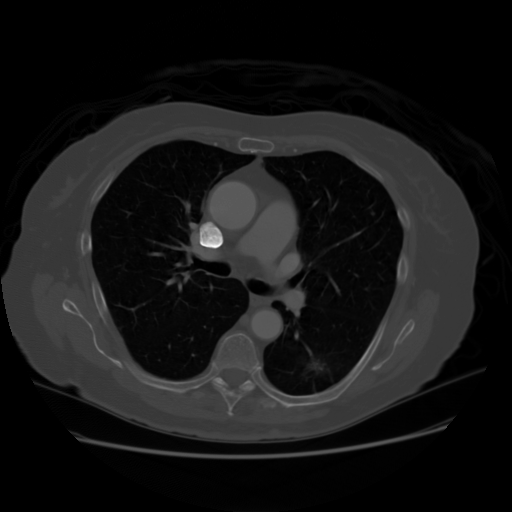
\includegraphics[width=0.5\textwidth]{../data/CT.png}
    \caption{Lung CT image from the LIDC-IDRI dataset.}
    \label{fig:lung_ct_image}
\end{figure}

\subsubsection{Image Characteristics}
The image shows a high contrast between the lungs and surrounding non lung tissue. This observation motivates a threshold based approach to segment the lung area. The nodules and tissue in the intra lung regions are of a much higher intensity than the lung tissue, as such it is appropriate supplement the thresholding step with additional morphological operations.

\subsubsection{Assumptions}
The algorithm assumes that after binarising the image via thresholding, the background makes up the largest connected component, with the left and right lungs being the next two largest. The algorithm also assumes that the nodules and tissue within the lung regions are fully enclosed and do not touch the border of the lung regions.

\subsubsection{Segmentation Algorithm}
\begin{itemize}
    \item \textbf{Binarise Image via Otsu Thresholding:} The image is thresholded using Otsu's threshold. This is a global thresholding method that maximises the inter-class variance of foreground and background. 
    \item \textbf{Connected Component Analysis:} The binary image is inverted to make the lung and background regions the foreground. The connected components of the inverted image are labelled using 8-connectivity. The second and third largest connected components are selected to recover the left and right lung regions. The connected components are selected based on their area. 
    \item \textbf{Binary Hole Filling} To recover the nodules and tissue within the lung regions, binary hole filling is performed. The algorithm fills holes in a binary image by inverting the image, labelling connected regions, and converting regions not connected to the border from background to foreground.
    \end{itemize}
    \begin{figure}[H]
        \centering
        \begin{subfigure}{.3\textwidth}
            \centering
            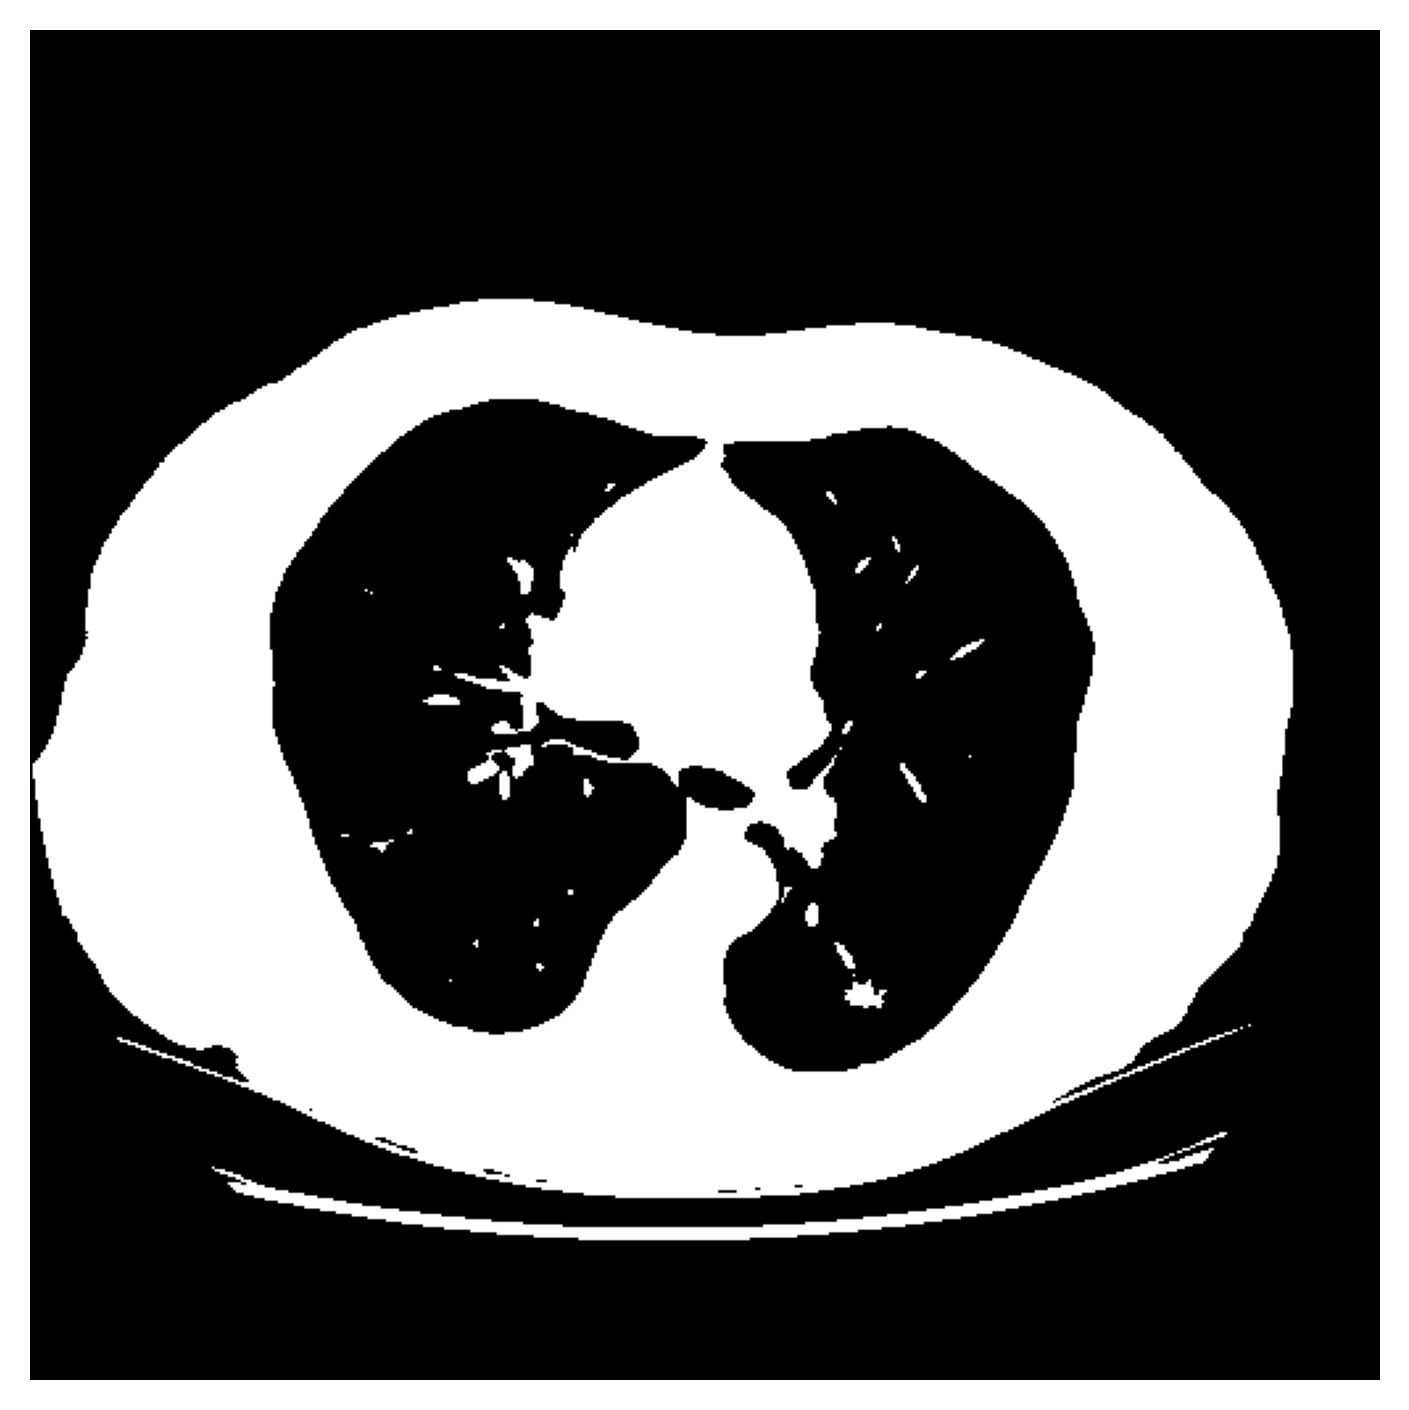
\includegraphics[width=\linewidth]{figs/q1a_binary.png}  % Replace with your image file
            \caption{}
            \label{fig:otsu_threshold}
        \end{subfigure}%
        \begin{subfigure}{.3\textwidth}
            \centering
            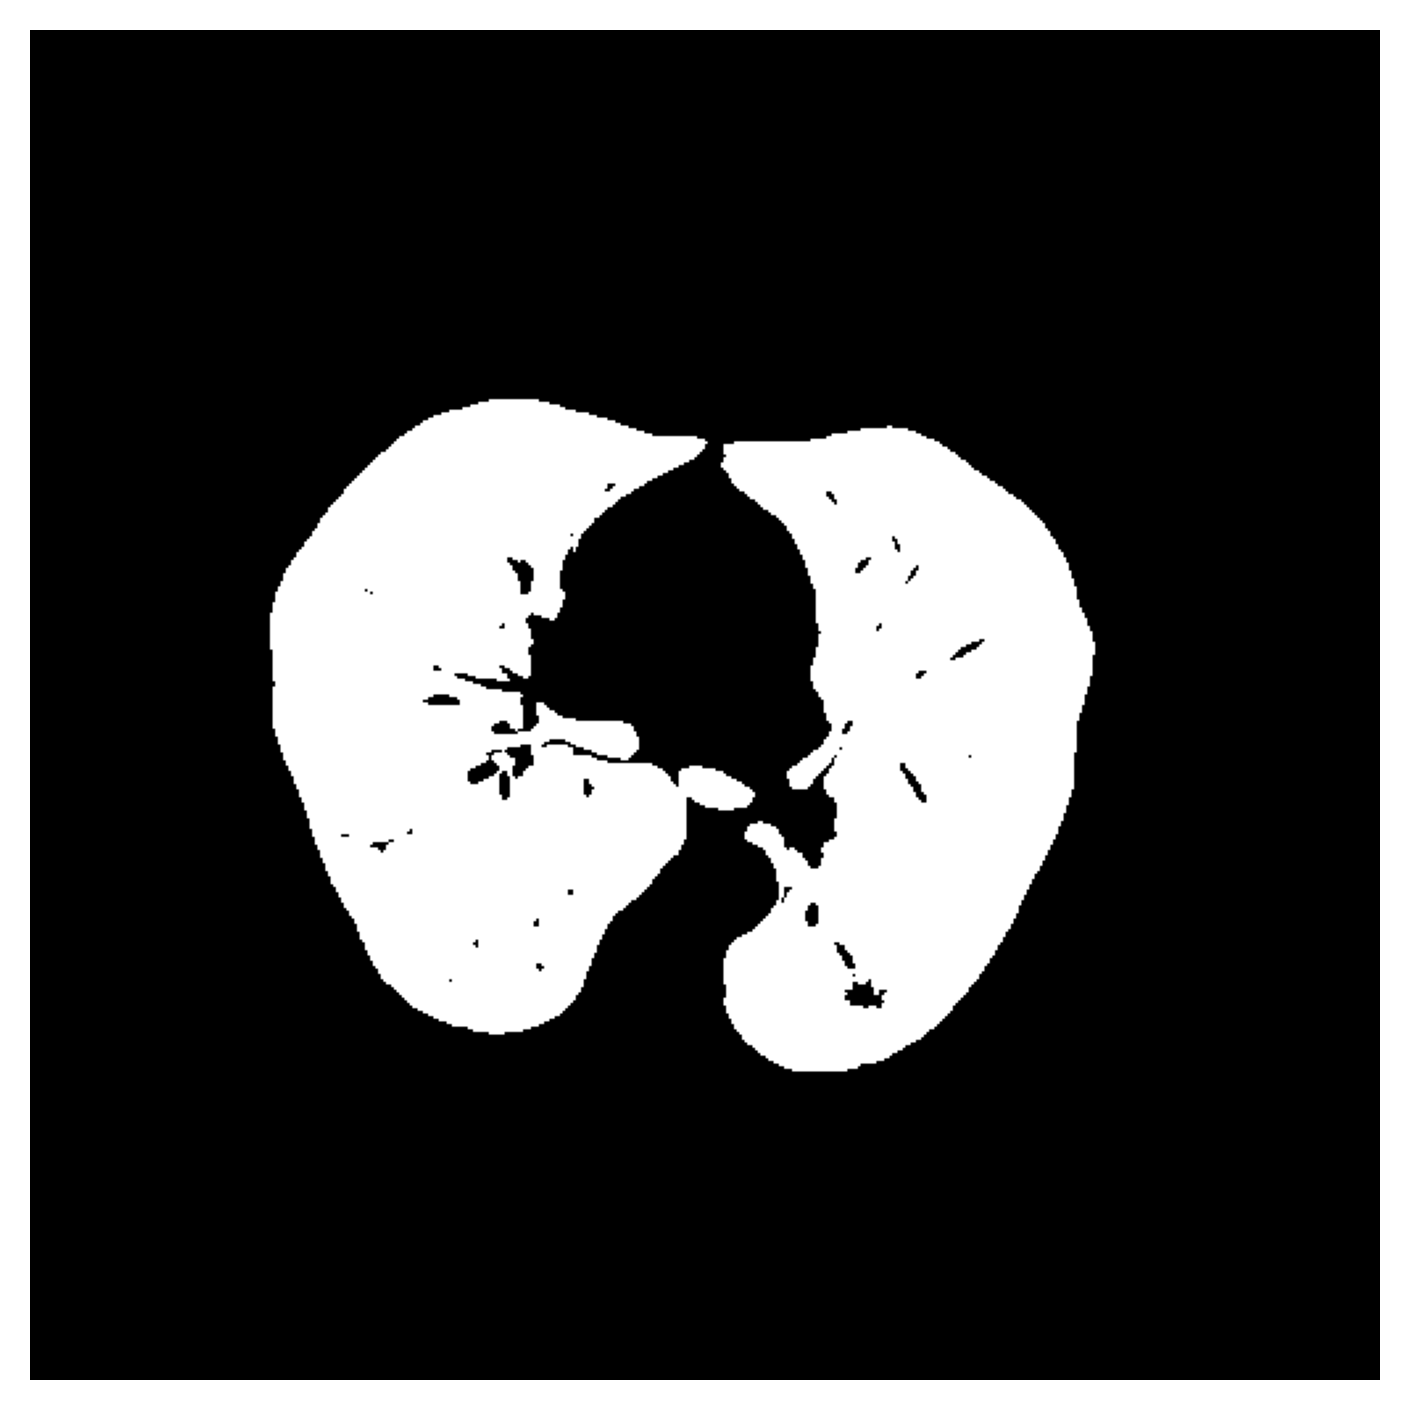
\includegraphics[width=\linewidth]{figs/q1a_largest_connected_components.png}  % Replace with your image file
            \caption{}
            \label{fig:connected_components}
        \end{subfigure}%
        \begin{subfigure}{.3\textwidth}
            \centering
            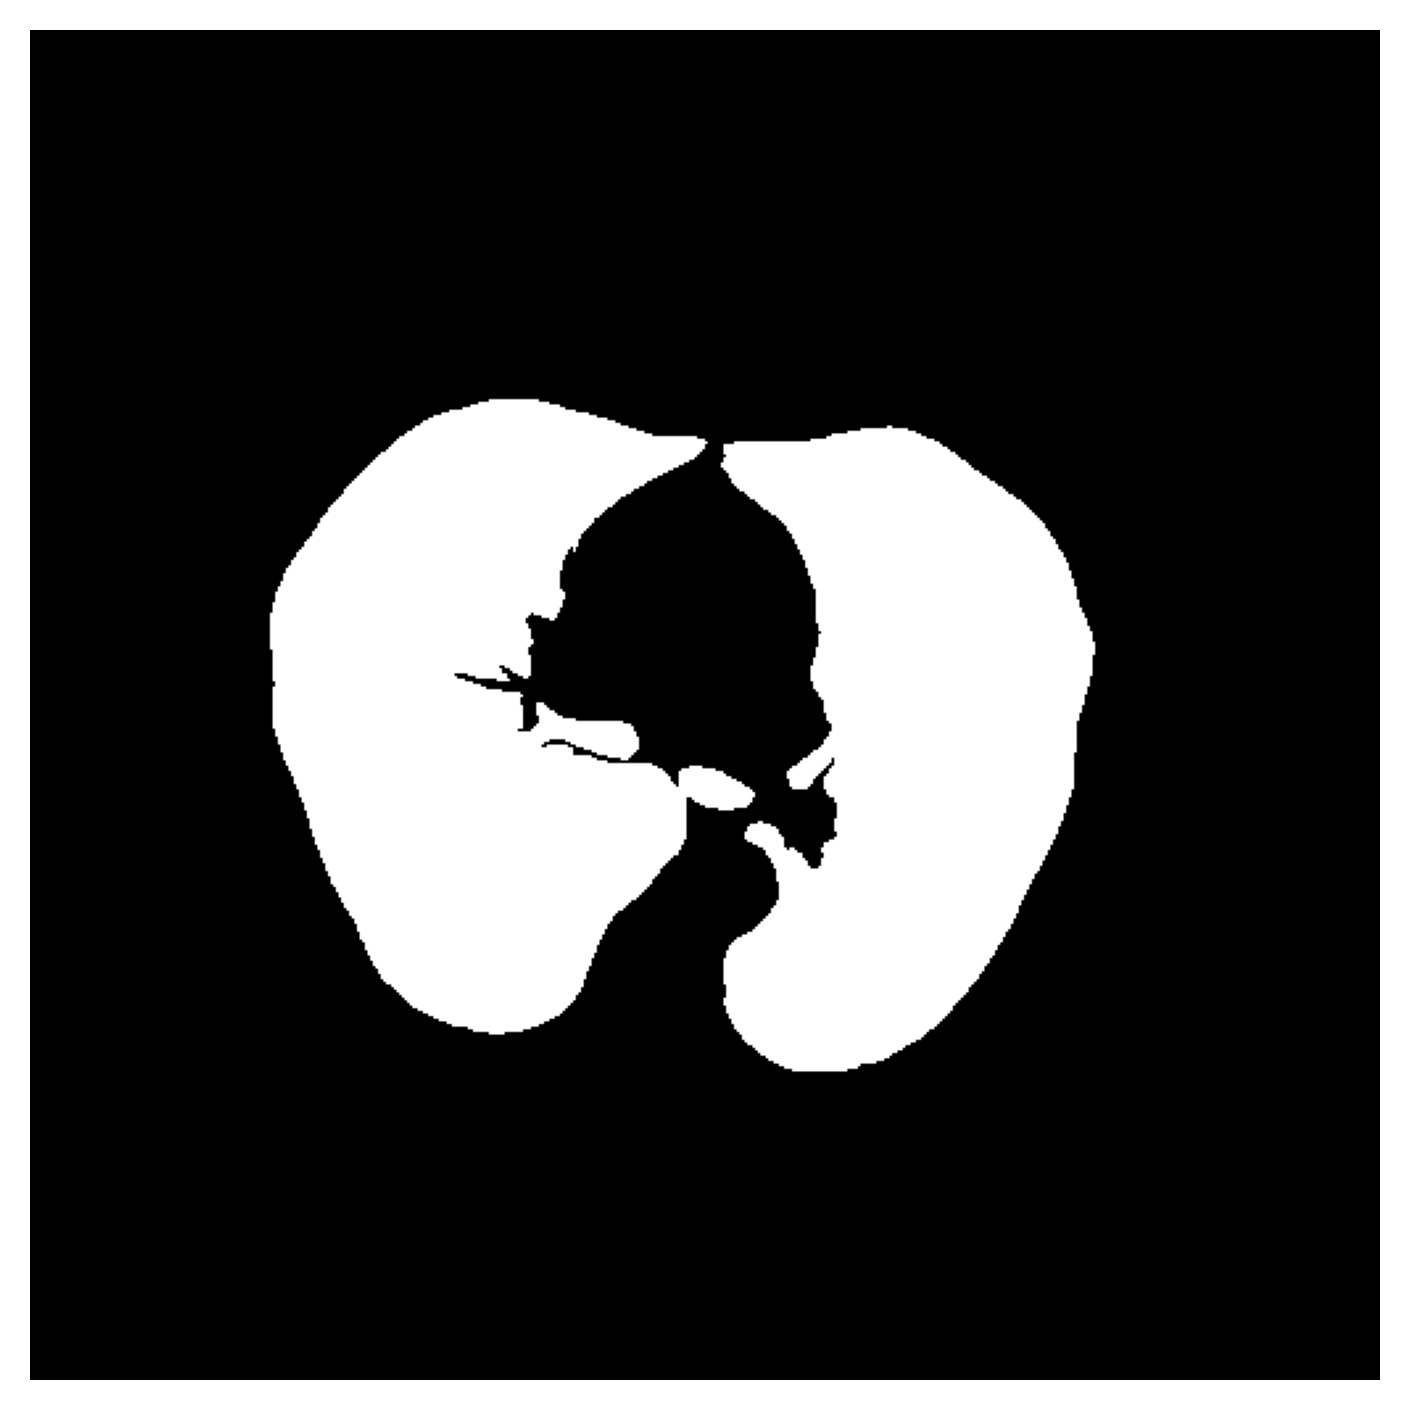
\includegraphics[width=\linewidth]{figs/q1a_filled_holes.png}  % Replace with your image file
            \caption{}
            \label{fig:filled_holes}
        \end{subfigure}
        \label{fig:segmentation_steps}
    \caption{Key steps in the segmentation of the lung CT image: (a) Binarisation using Otsu's threshold, (b) Mask inversion and selection of lung regions via connected component analysis, (c) Recovery of internal structures through binary hole filling.}
    \end{figure}
Note, this segmentation algorithm was also implemented from scratch. Relevant code can be found in \texttt{src/q1a\_from\_scratch.py} and \texttt{src/from\_scratch\_seg\_funcs.py}.
\subsubsection{Results}
The final segmentation of the lung CT image is shown in Figure \ref{fig:lung_ct_image} The segmentation clearly captures the relevant lung regions and all the nodules and tissues within.
\begin{figure}[H]
    \centering
    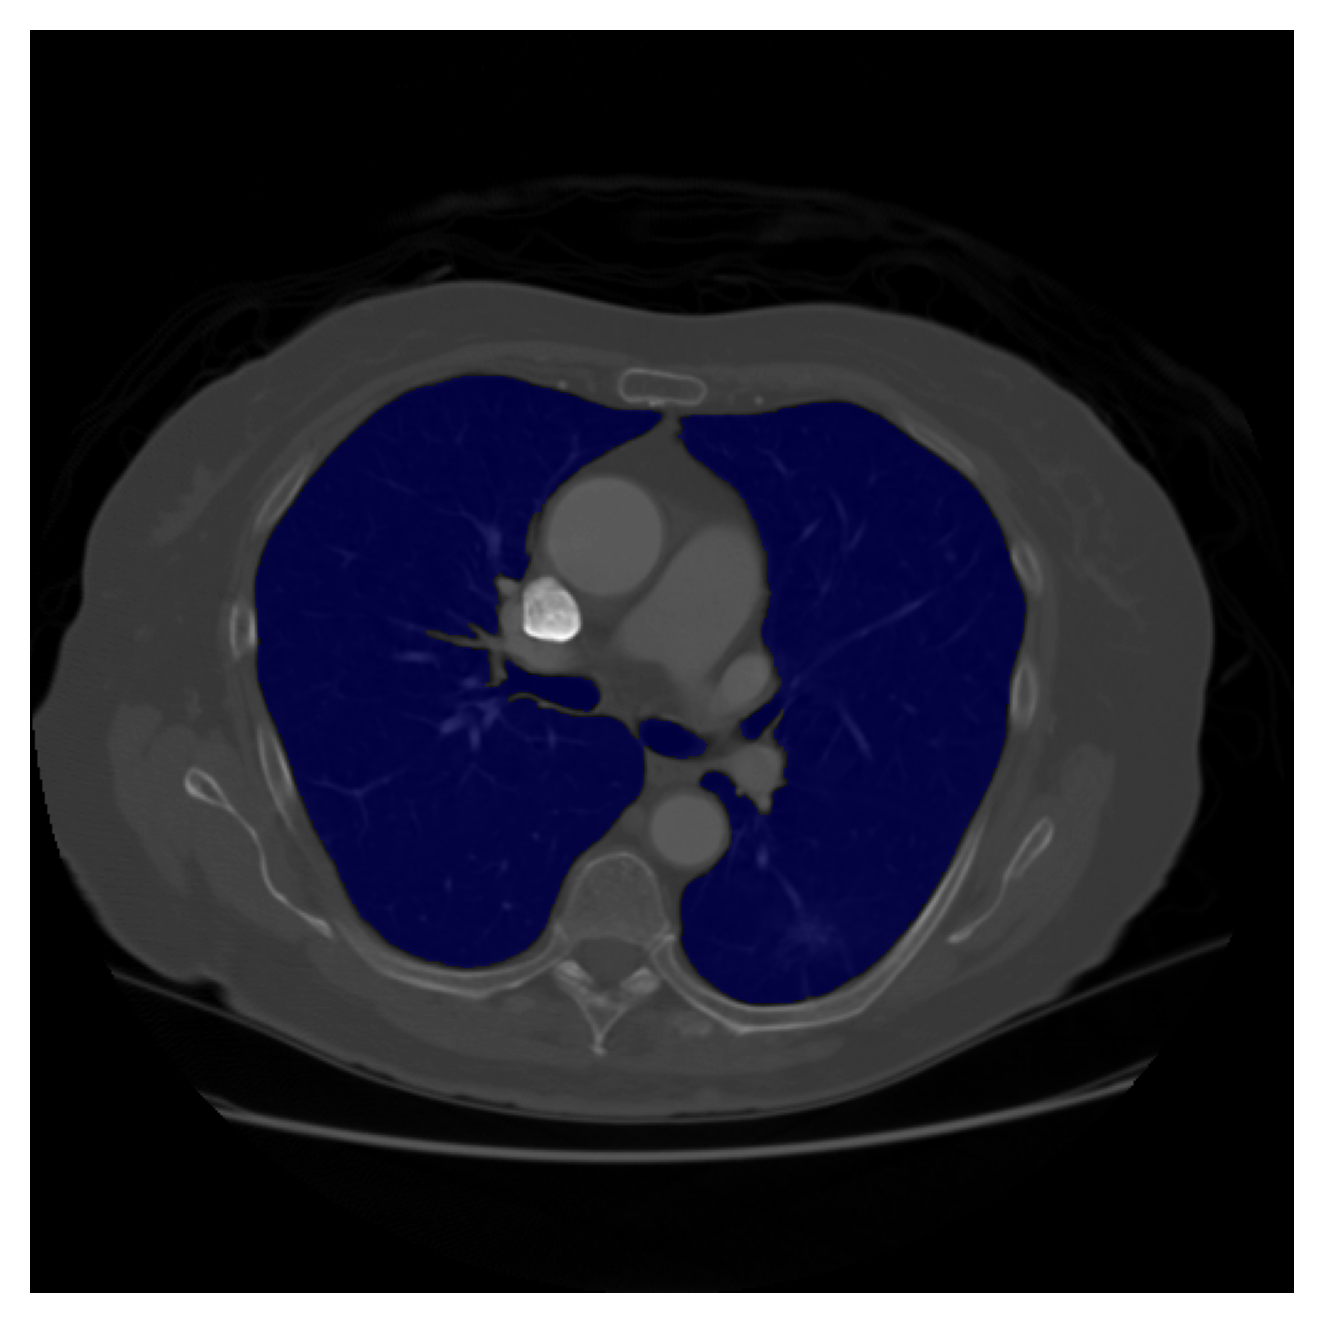
\includegraphics[width=0.4\textwidth]{figs/q1a.png}
    \caption{Final segmentation of the lung CT image.}
    \label{fig:lung_ct_segmentation}
\end{figure}

\subsubsection{Discussion}
Figure \ref{fig:q1a_ambiguity} shows a potential ambiguous region in the segmentation. This region was segmented due to having a similar intensity as the lung tissue and being connected to lung tissue post Otsu thresholding. However, as this region could not be clearly identified as non lung tissue without additional context, it was kept in the final segmentation. This also highlights the limitations of thresholding based segmentation methods in identifying regions that are not clearly defined by intensity.
\begin{figure}[H]
    \centering
    \begin{subfigure}{.4\textwidth}
        \centering
        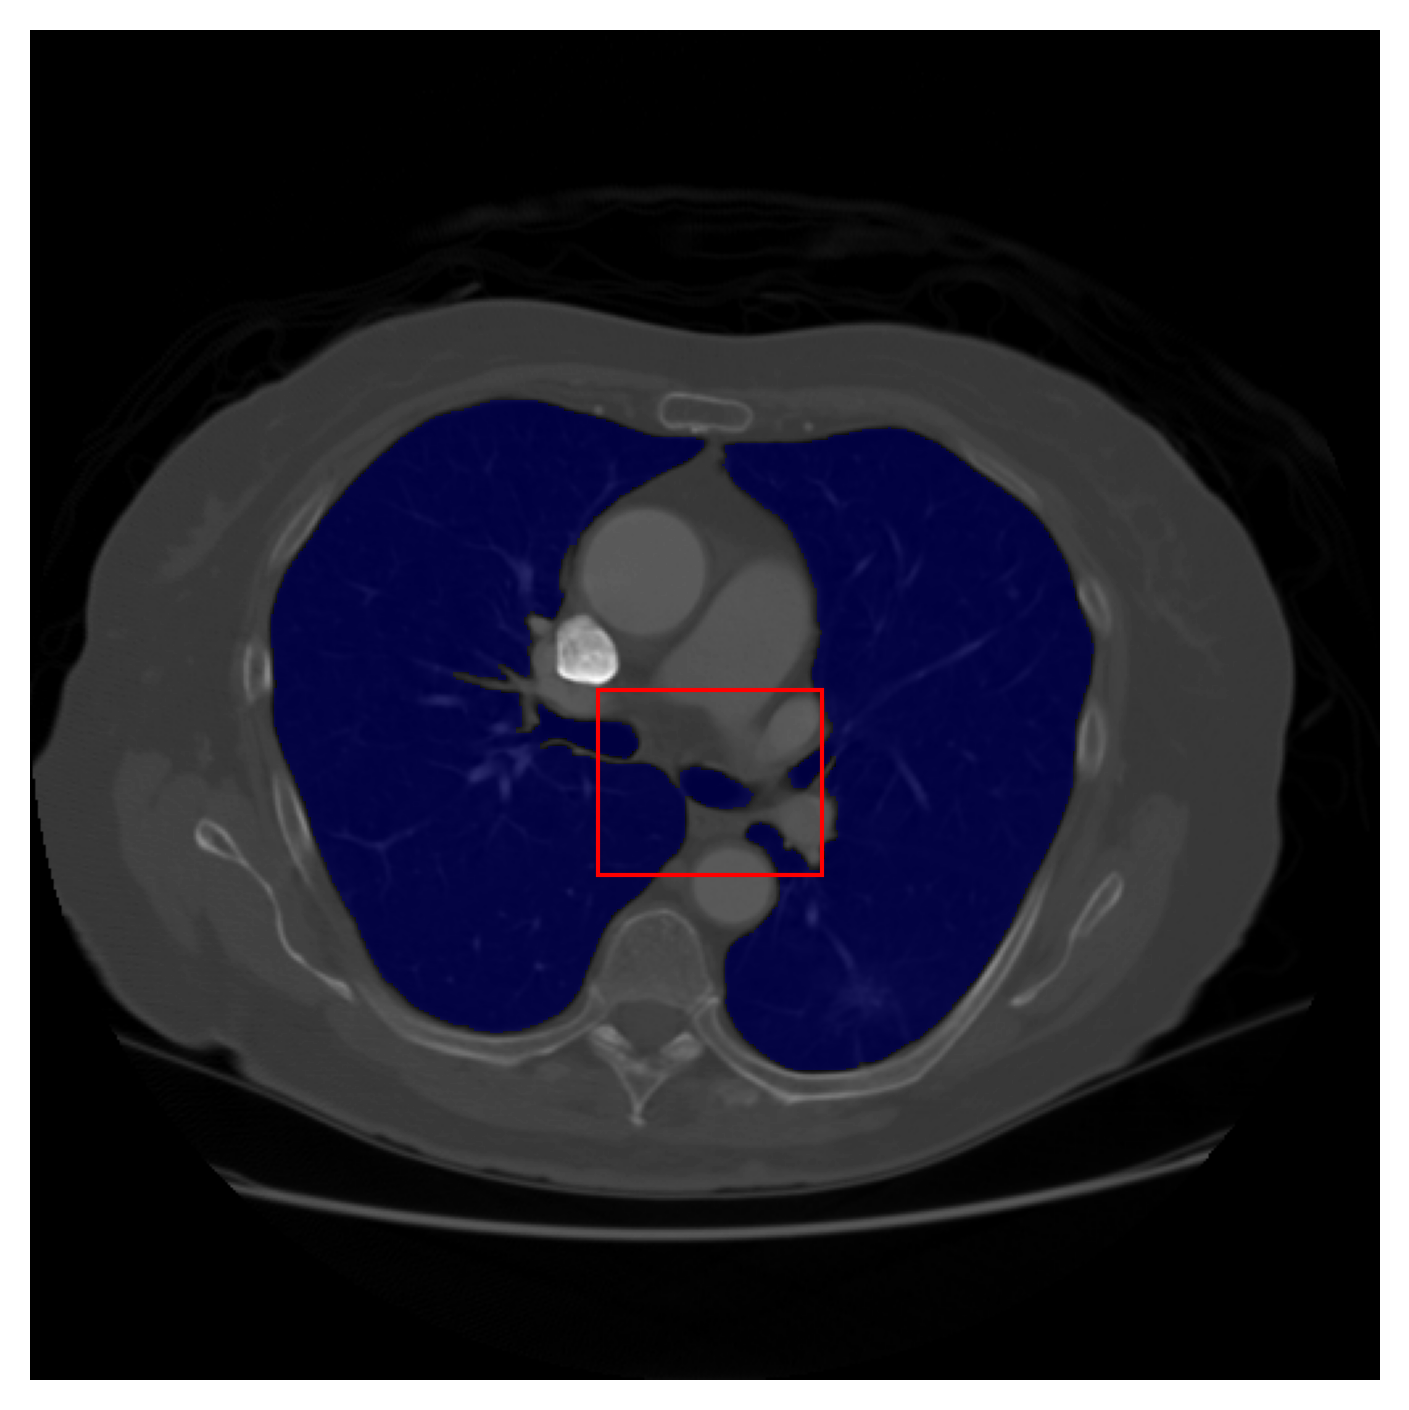
\includegraphics[width=\linewidth]{figs/q1a_seg_w_bbox.png}  % Replace with your image file
        \caption{}
        \label{fig:q1a_seg_w_bbox}
    \end{subfigure}%
    \begin{subfigure}{.4\textwidth}
        \centering
        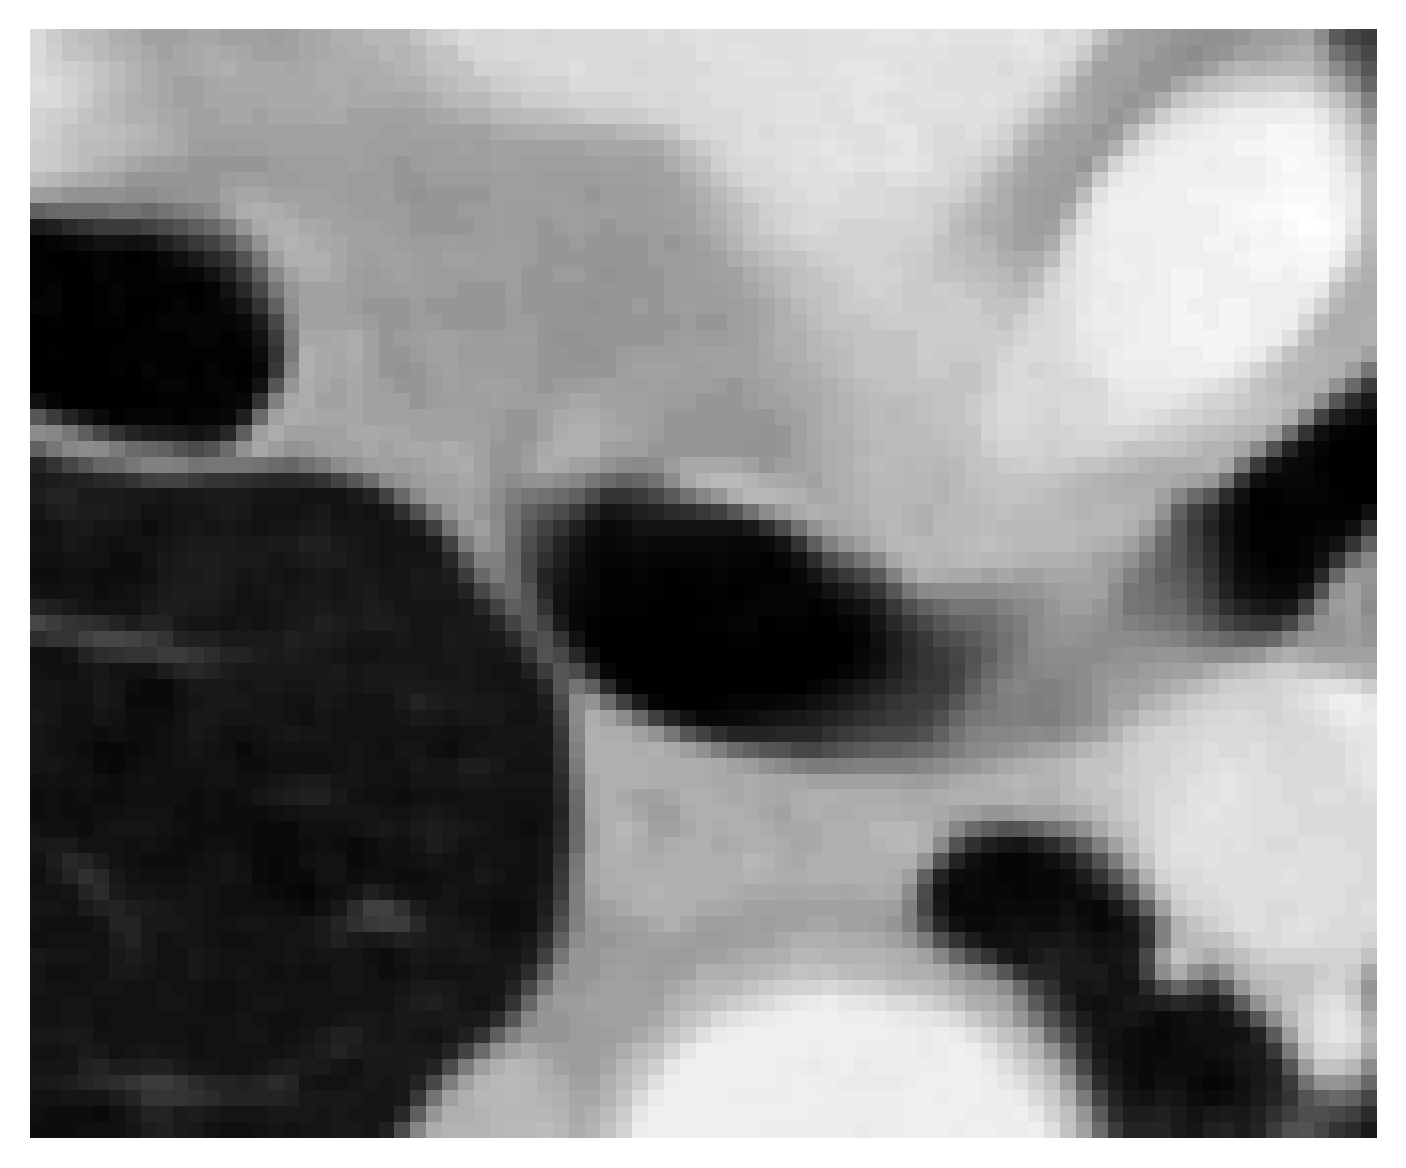
\includegraphics[width=\linewidth]{figs/q1a_zoomed_region.png}  % Replace with your image file
        \caption{}
        \label{fig:q1a_zoomed_region}
    \end{subfigure}%
    \caption{Ambiguous region in the segmentation: (a) Segmentation with bounding box around the ambiguous region, (b) Zoomed in view of the ambiguous region.}
    \label{fig:q1a_ambiguity}
\end{figure}

\subsection{Part B: Noisy Flowers Image Segmentation}
This section details the segmentation algorithm of the noisy flowers image shown in Figure \ref{fig:flowers_image}. The region to be segmented are all the purple flower heads in the image.

\begin{figure}[H]
    \centering
    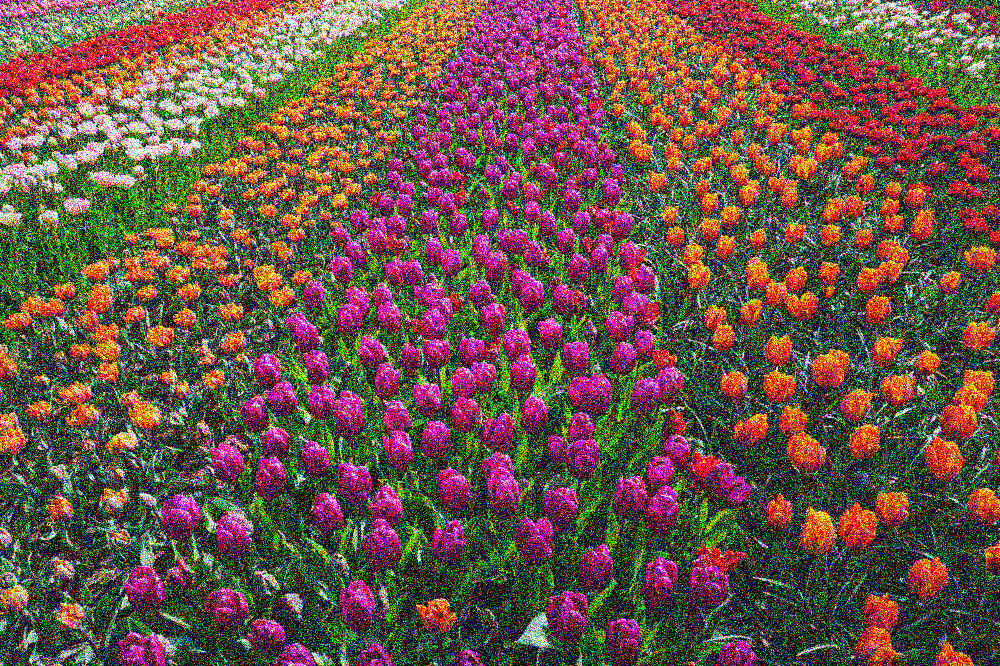
\includegraphics[width=0.8\textwidth]{../data/noisy_flower.jpg}
    \caption{Noisy Flowers image.}
    \label{fig:flowers_image}
\end{figure}

\subsubsection{Image Characteristics}
The image features a type of noise that is typical to gaussian degradations. This was confirmed by applying a gaussian filter to each of the colour channels seperately in the image and observing that nearby pixel colours were more. This effect is shown in Figure \ref{fig:gaussian_noise_evidence}. 
\begin{figure}[H]
    \centering
    \begin{subfigure}{.4\textwidth}
        \centering
        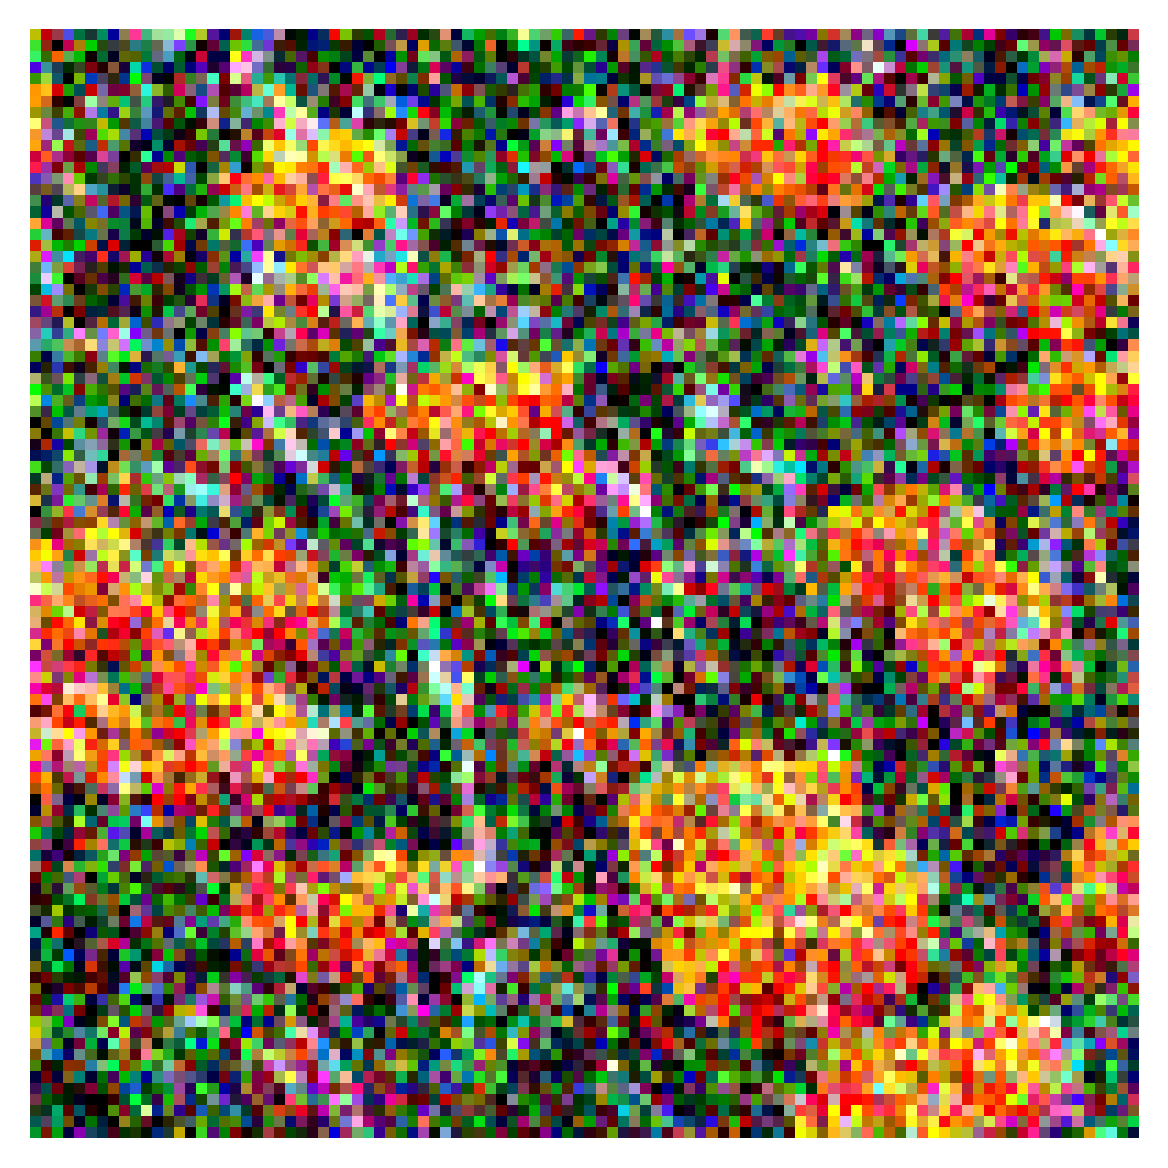
\includegraphics[width=\linewidth]{figs/q1b_patch.png}  % Replace with your image file
        \caption{}
        \label{fig:flower_patch}
    \end{subfigure}%
    \begin{subfigure}{.4\textwidth}
        \centering
        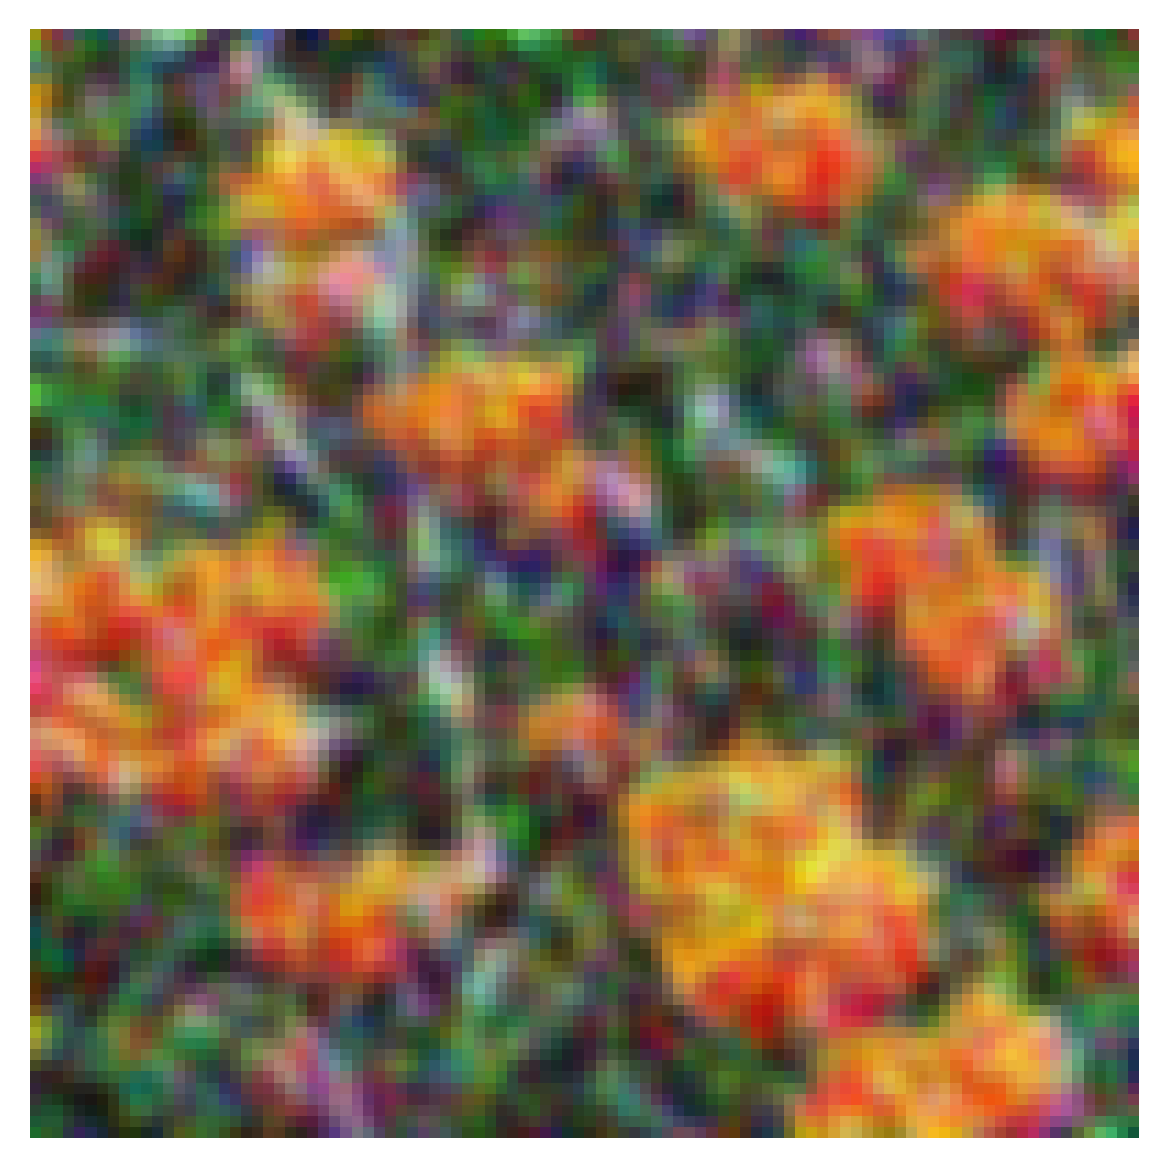
\includegraphics[width=\linewidth]{figs/q1b_gauss_blurred_patch.png}  % Replace with your image file
        \caption{}
        \label{fig:gaussian_filtered_flower_patch}
    \end{subfigure}%
    \caption{Effect of Gaussian filtering on the colour channels of the noisy flowers image: (a) Cropped region of the noisy flowers image, (b) Cropped region after applying a Gaussian filter with standard deviation 1.}
    \label{fig:gaussian_noise_evidence}
\end{figure}
The purple flowers in \ref{fig:flowers_image}, except for the ones clearly in the foreground, are all roughly of the same shade of purple. There are two batches of purple flowers in the image, one large group down the middle and another smaller group along the upper left corner of the image. The purple flowers in the foreground have shadows on them making the bottom half of the flower darker than the top half. Due to the general uniformity in colours of the flower after denoising, a clustering type algorithm is appropriate for this image.

\subsubsection{Assumptions}
The main assumption made by this algorithm is in choosing the number of clusters. The number of clusters is chosen to be 5, which is chosen based on the number of distinct colours in the image. The green grass and stems, the orange flower heads, the purple flower heads, the white flower heads and the red flower heads.

\subsubsection{Segmentation Algorithm}
\begin{itemize}
    \item \textbf{Bilateral Gaussian Filtering:} First the image was denoised using a bilateral filter \cite{710815}. This filter was chosen for its ability to denoise while considering both spatial proximity and colour similarity, ideal for preserving flower head edges. A spatial standard deviation of 15 was chosen to allow for smoothing across the entire flower head regions, while a colour standard deviation of 1 ensures edge sharpness by only blending similarly coloured pixels. This approach effectively reduces noise without blurring distinct colour boundaries.
    \item \textbf{Conversion from RGB to LAB colour Space:} The image is converted from RGB to LAB colour space, which better approximates human vision by separating colour and luminance. This space enhances clustering accuracy because Euclidean distances more closely reflect perceptual differences, making it ideal for grouping similar colours like purple flower heads.
    \item \textbf{K-Means Clustering:} K-means clustering is applied to the LAB image. The number of clusters is chosen to be 5, based on the number of distinct colours in the image. The image is then segmented by assigning each pixel to the cluster with the closest centroid.
    \item \textbf{Select Purple Pixels} The cluster centre closest to the the LAB value of purple is chosen to be the desired cluster to represent the foreground. The image is binarised by setting all pixels not in this cluster to 0 and all pixels in this cluster to 1.
    \item \textbf{Denoise Segmentation via Morphological Opening} To remove small-scale noise from the mask while retaining the shape and size of the main flower heads, a morphological opening operation is applied. 
    \item \textbf{Remove Small Connected Components:} Finally to remove any left over noise, all connected components with an area less than 100 pixels are removed. The previous morphological opening step ensures the required thresholding does not remove any of the main flower heads.
\end{itemize}
\begin{figure}[H]
    \centering
    \begin{subfigure}{.45\textwidth}  % Adjusted to fit two figures per row
        \centering
        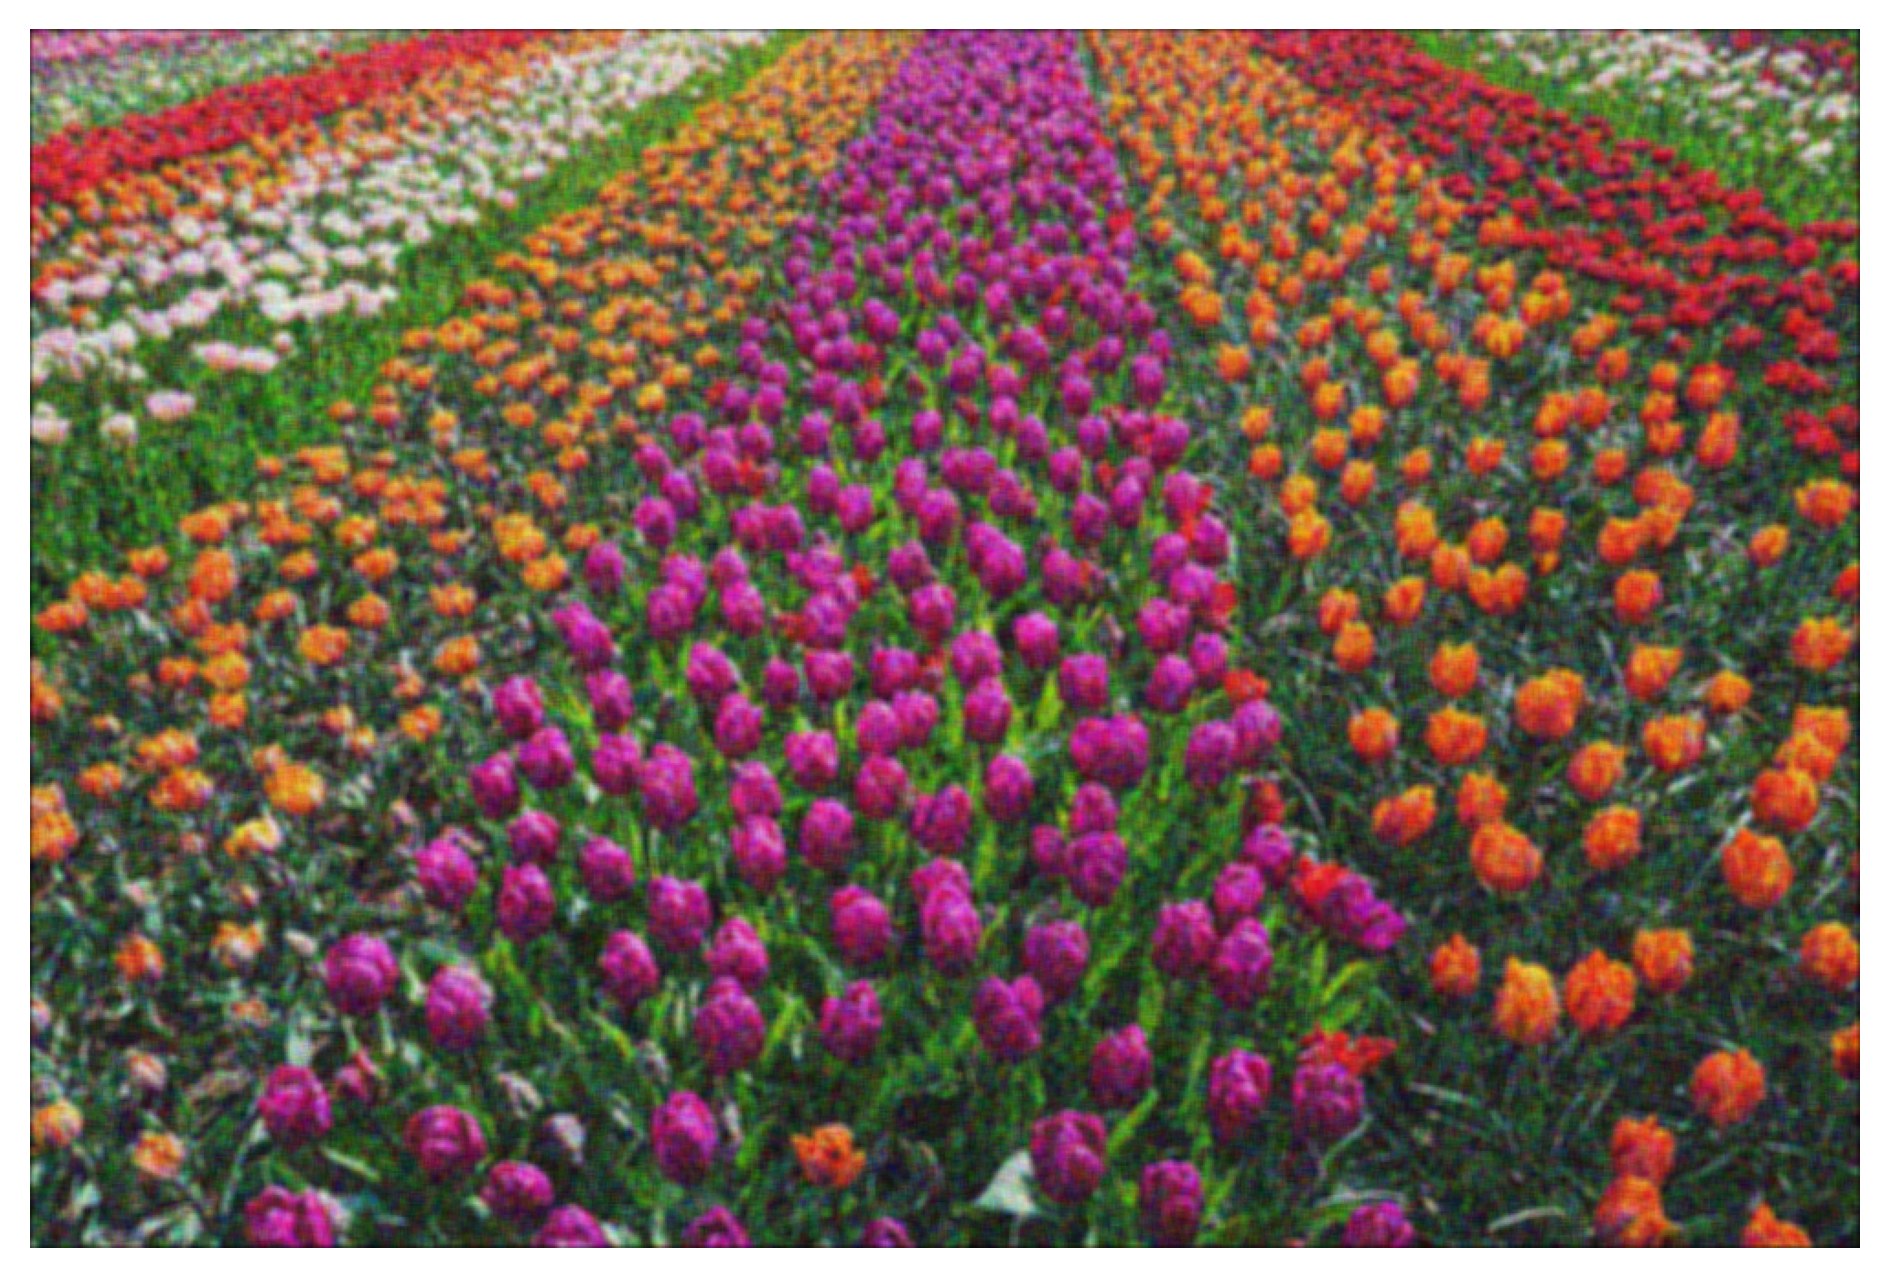
\includegraphics[width=\linewidth]{figs/q1b_denoised.png}
        \caption{}
        \label{fig:denoised_flowers}
    \end{subfigure}%
    \begin{subfigure}{.45\textwidth}  % Adjusted to fit two figures per row
        \centering
        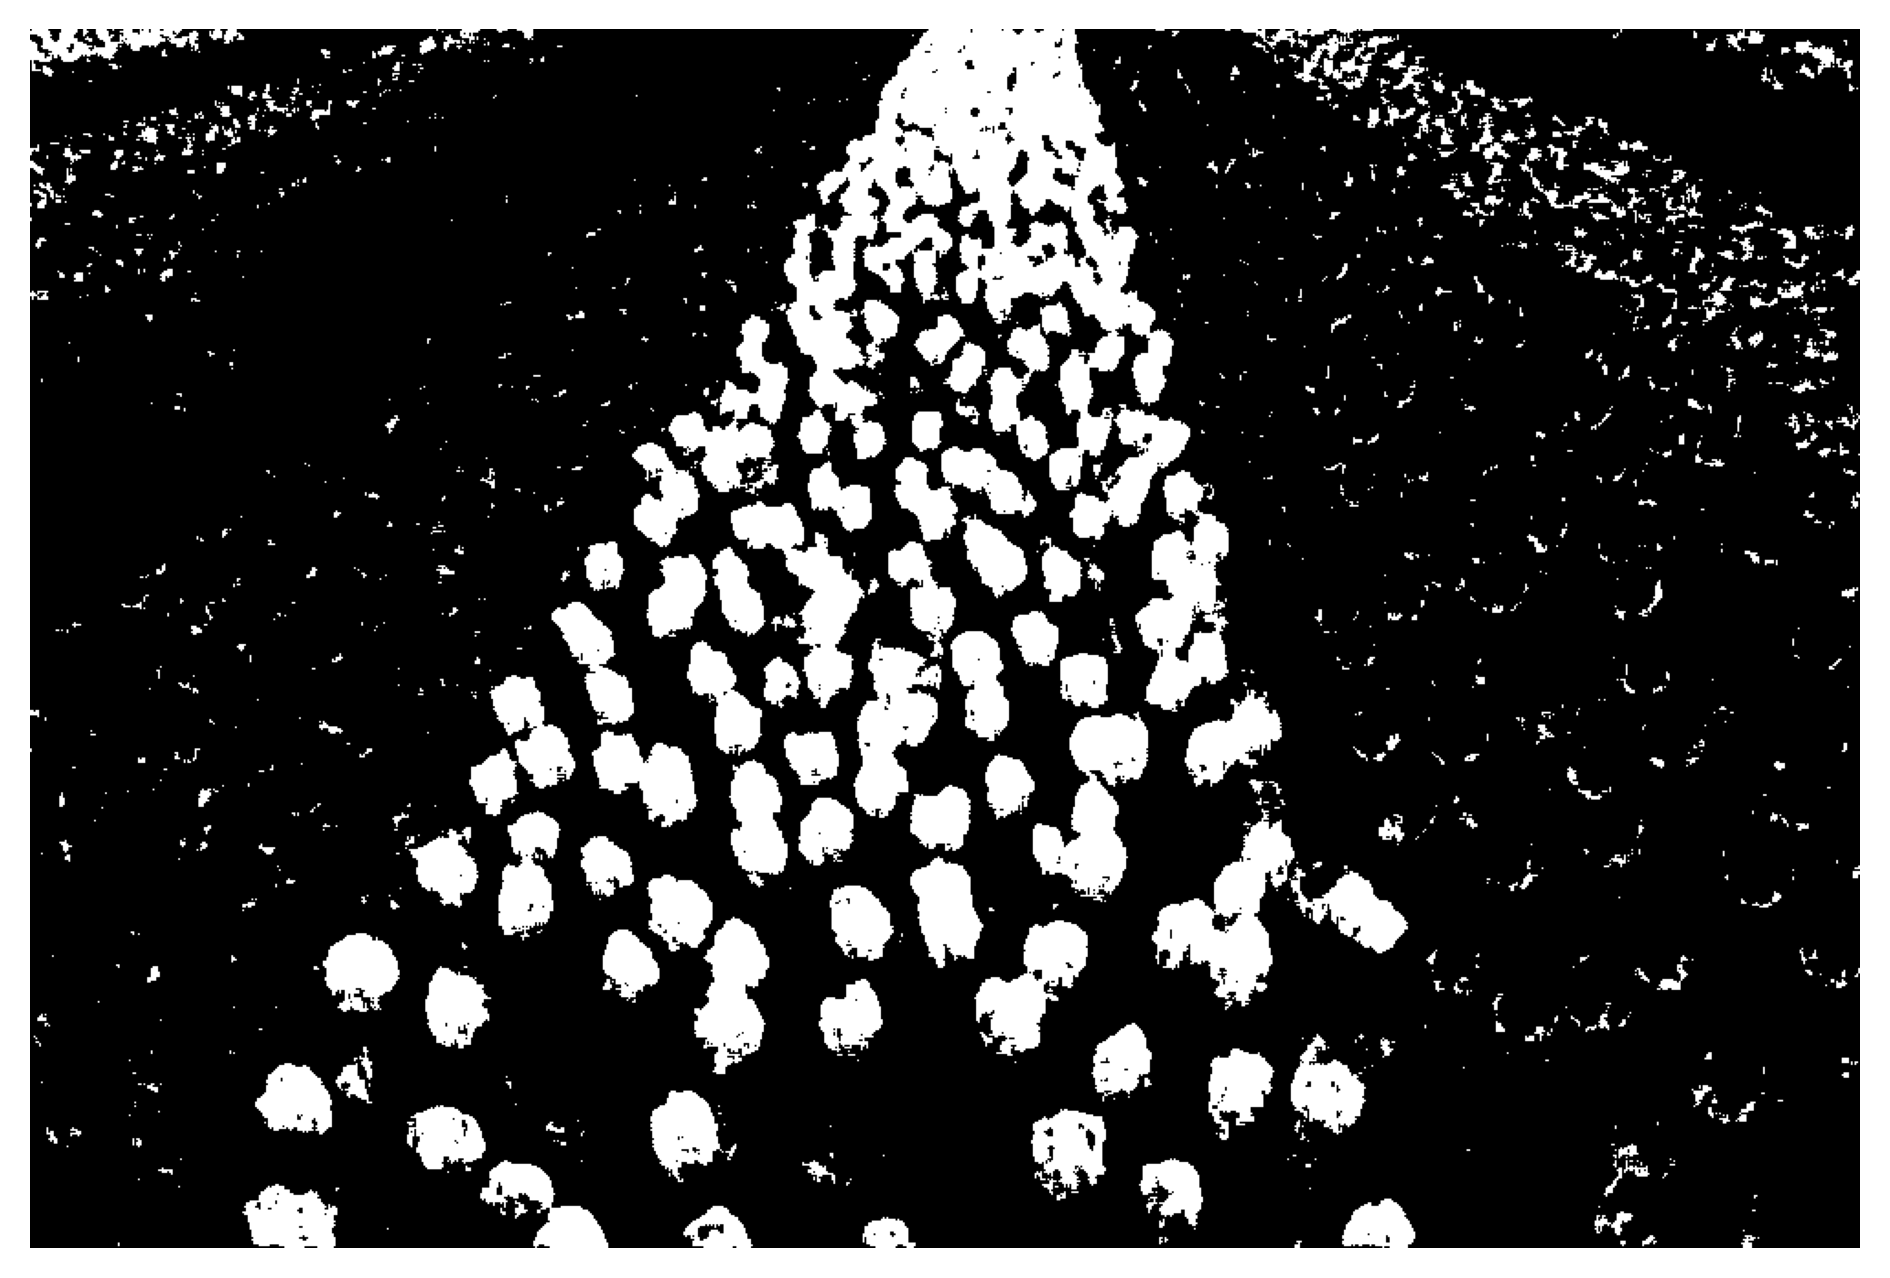
\includegraphics[width=\linewidth]{figs/q1b_kmeans_mask.png}
        \caption{}
        \label{fig:kmeans_mask_flowers}
    \end{subfigure}
    \begin{subfigure}{.45\textwidth}  % New row, first column
        \centering
        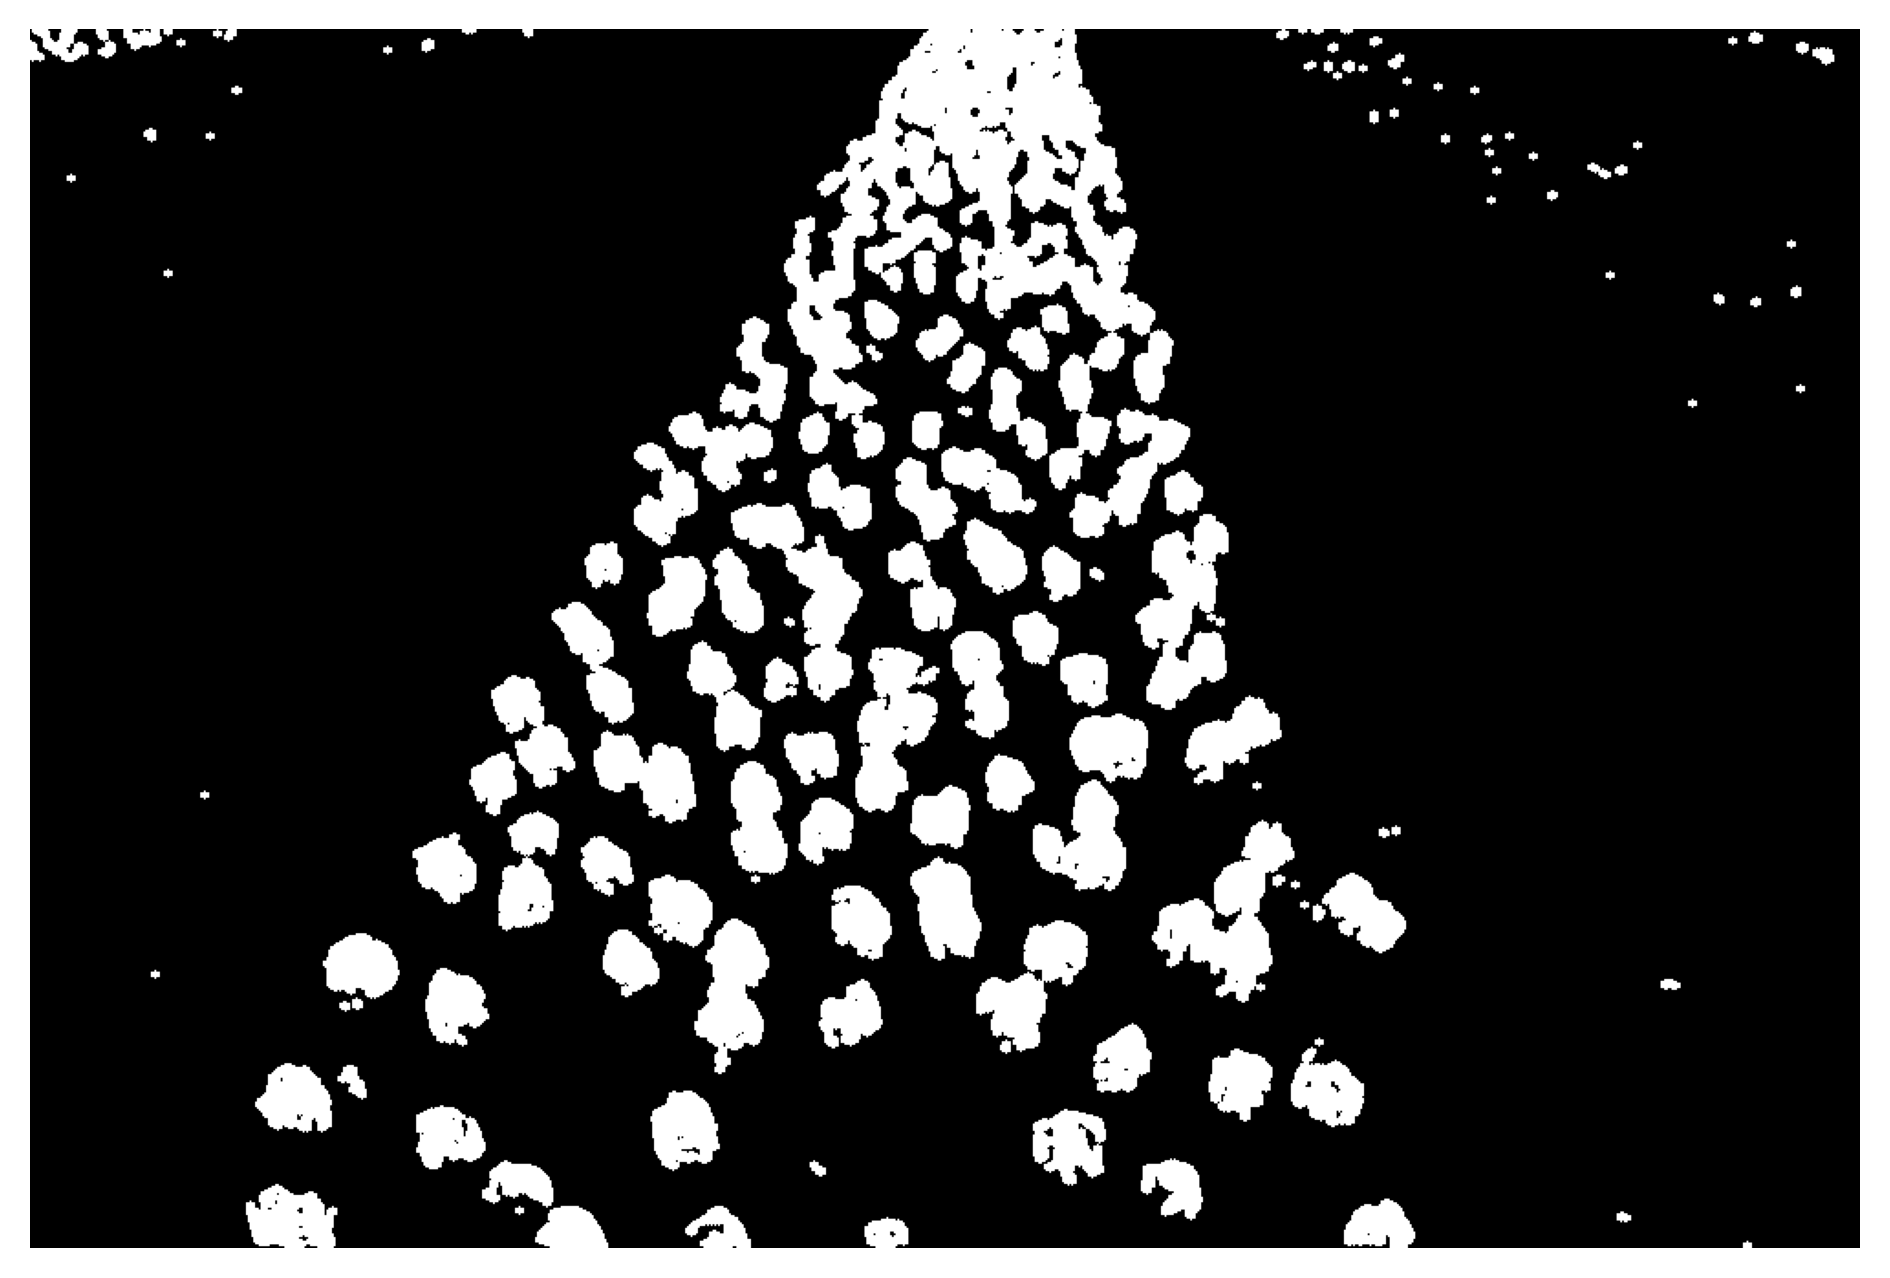
\includegraphics[width=\linewidth]{figs/q1b_kmeans_mask_post_opening.png}
        \caption{}
        \label{fig:kmeans_mask_post_opening_flowers}
    \end{subfigure}%
    \begin{subfigure}{.45\textwidth}  % New row, second column
        \centering
        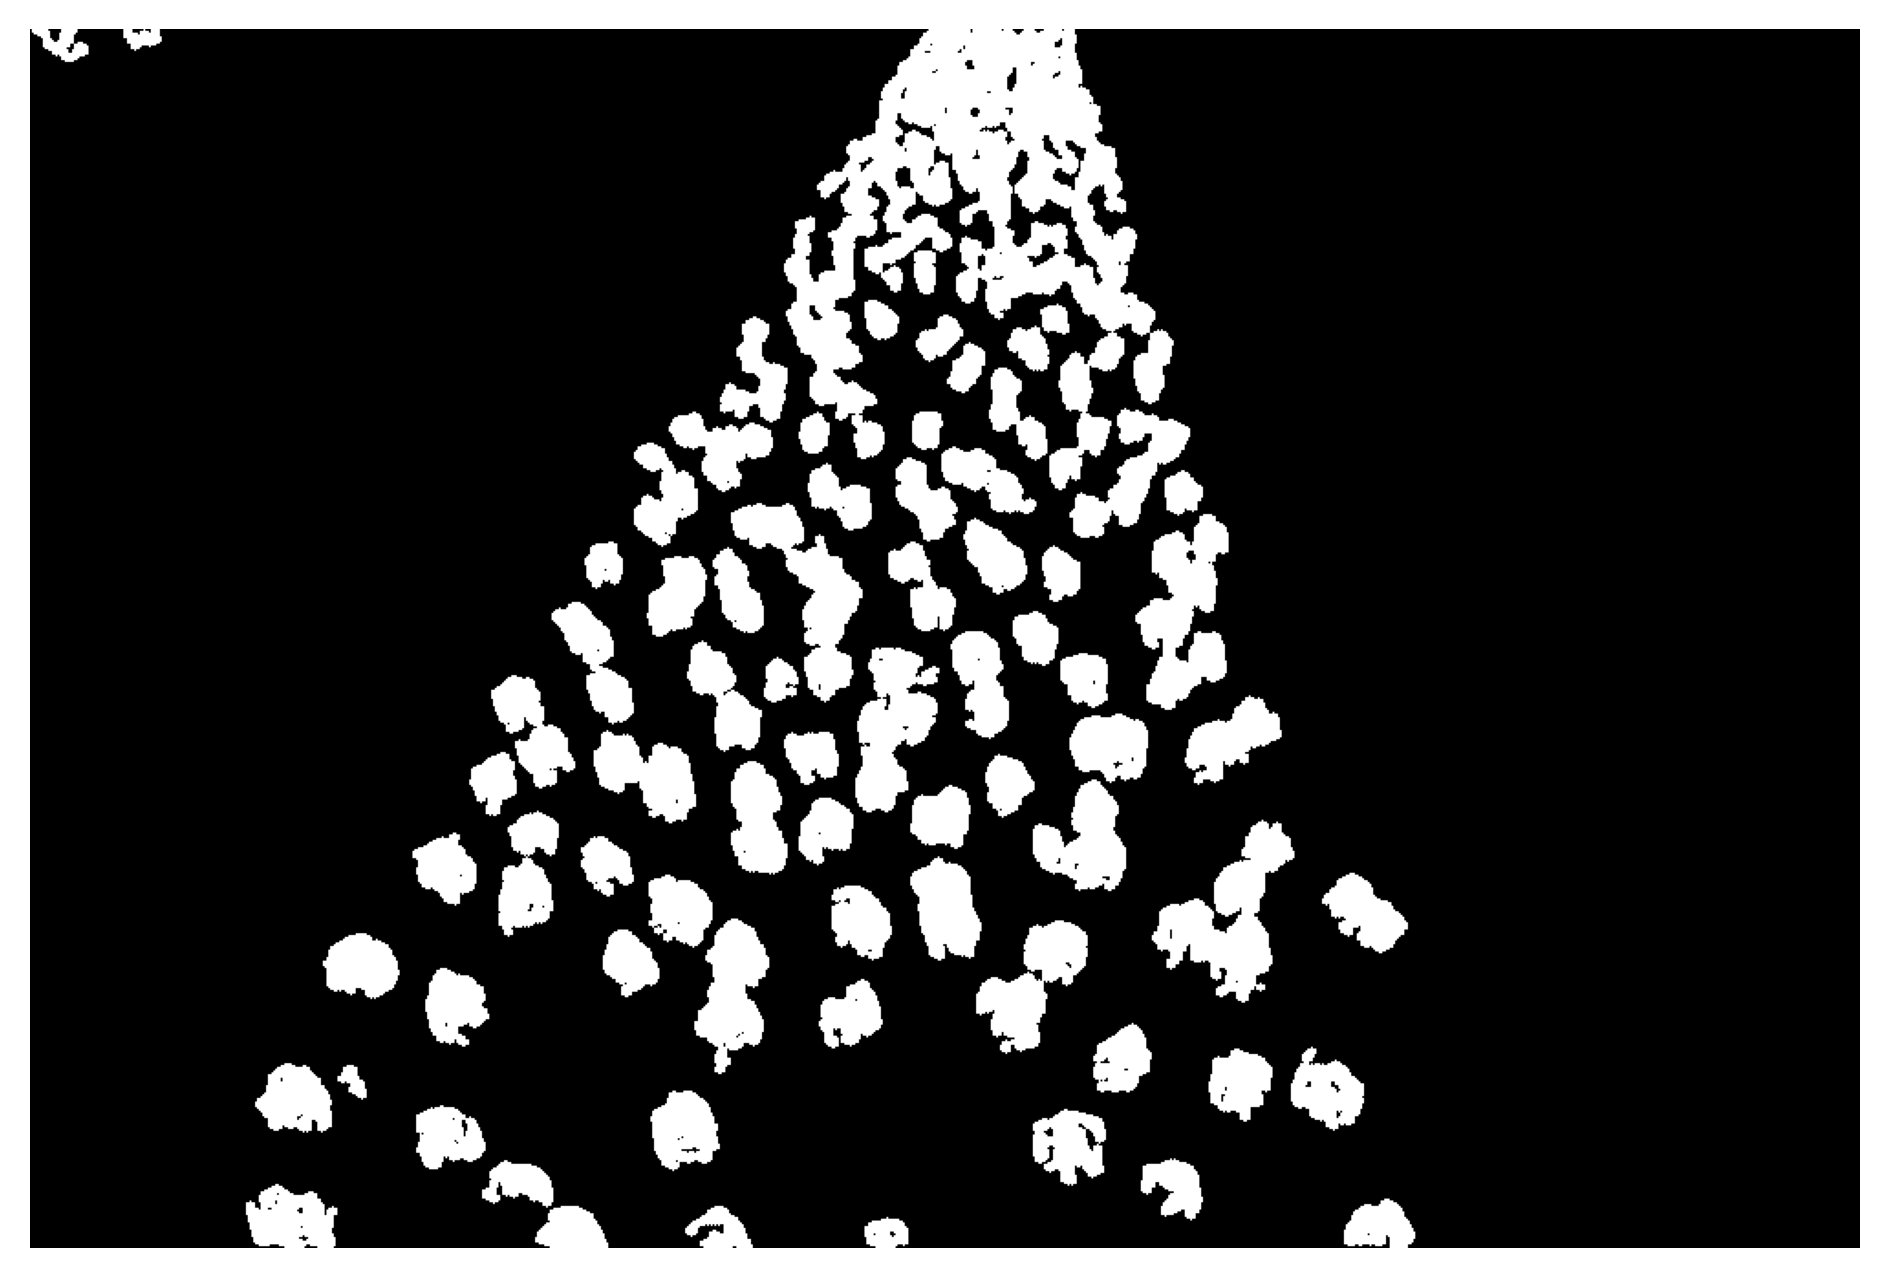
\includegraphics[width=\linewidth]{figs/q1b_mask_post_cnc_removal.png}
        \caption{}
        \label{fig:cnc_threshold_flowers}
    \end{subfigure}%
    \caption{Segmentation process for the noisy flowers image: (a) Image after denoising with a bilateral filtering, showing reduced colour noise while preserving edge details. (b) Result of applying K-means clustering to segment purple pixels. (c) Segmentation mask post morphological opening, illustrating reduced noise in the segmentation. (d) Final segmentation after removing small connected components, highlighting the refined segmentation of flower regions.}
    \label{fig:q1b_segmentation_steps}
\end{figure}

\subsubsection{Results}
The final segmentation of the noisy flowers image is shown in Figure \ref{fig:q1b_final_mask}. The segmentation clearly captures most of the purple flower heads in the main central bunch. It also captures some in the smaller bunch in the upper left corner. It is able to distinguish between the colours effectively, with some of the orange and red flowers in the purple group being excluded from the segmentation quite effectively as seen in figure \ref{fig:flowers_seg_zoomed}.

\begin{figure}[H]
    \centering
    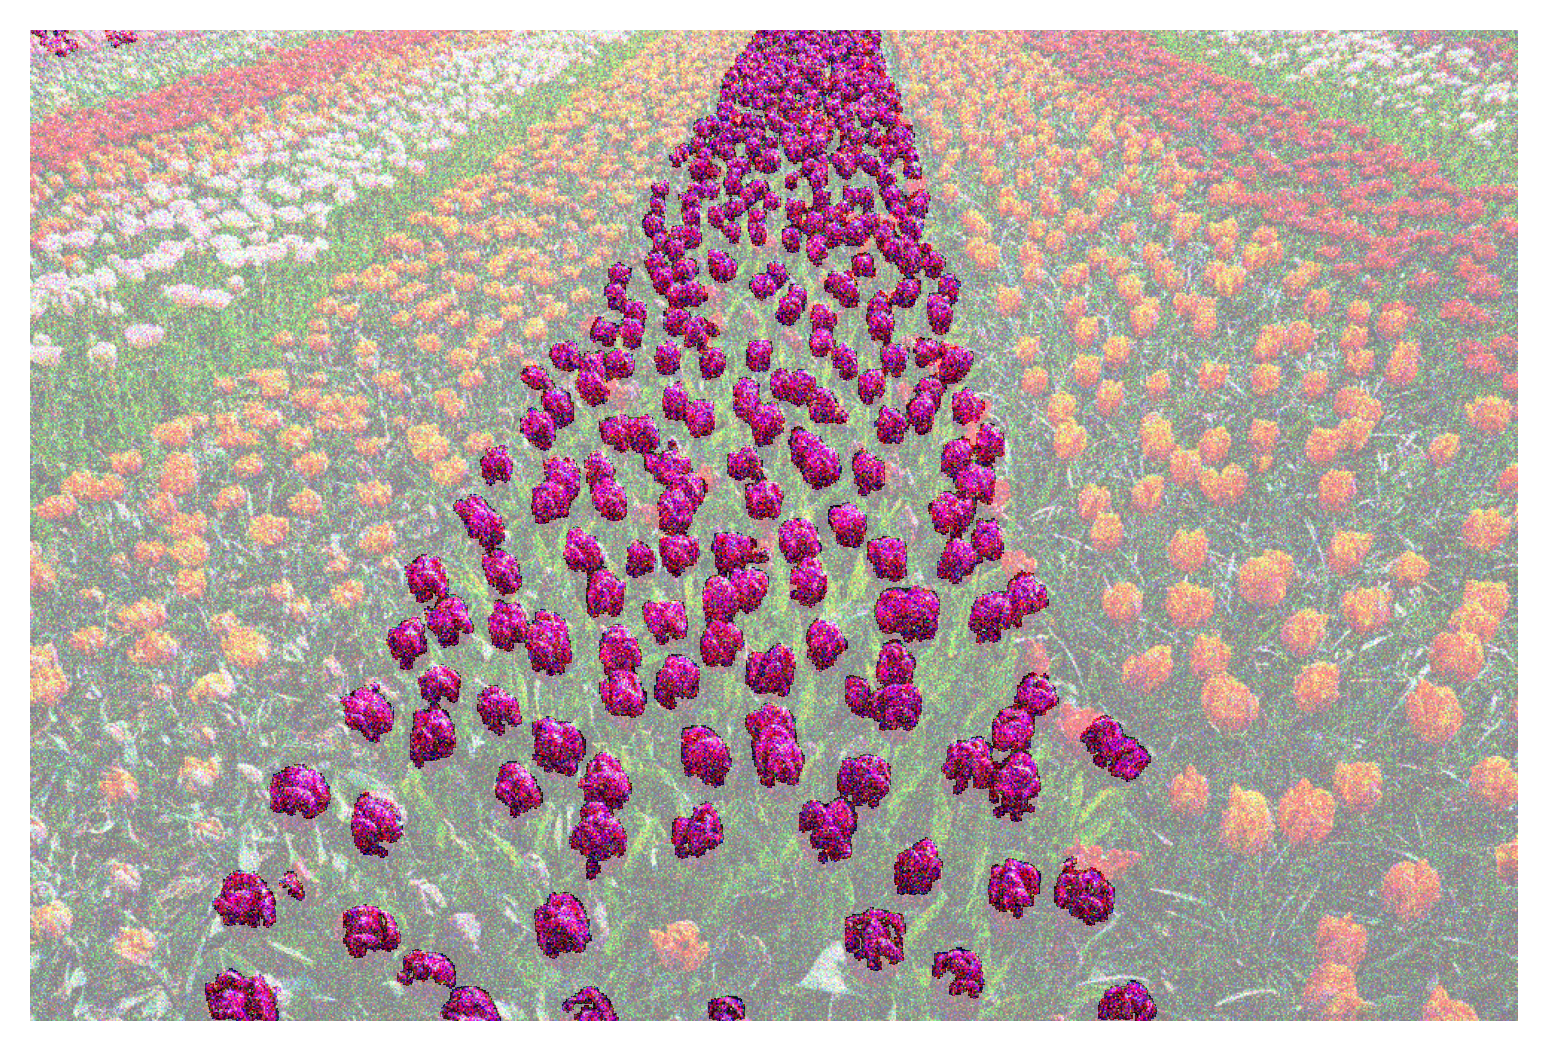
\includegraphics[width=0.8\textwidth]{figs/q1b_final_mask.png}
    \caption{Final segmentation of the noisy flowers image.}
    \label{fig:q1b_final_mask}
\end{figure}

% TODO: Think of a better colouring scheme for the bounding boxes, white is washing out the image.
\begin{figure}[H]
    \centering
    \begin{subfigure}[c]{.6\textwidth}  % Centered subfigure on the left
        \centering
        \includegraphics[width=\linewidth]{figs/q1b_seg_w_good_bbox.png}
        \caption{}  % Caption for the left subfigure
        \label{fig:q1b_zoomed}
    \end{subfigure}%
    \begin{minipage}[c]{.35\textwidth}  % Centered minipage for the right subfigures
        \begin{subfigure}{\textwidth}
            \centering
            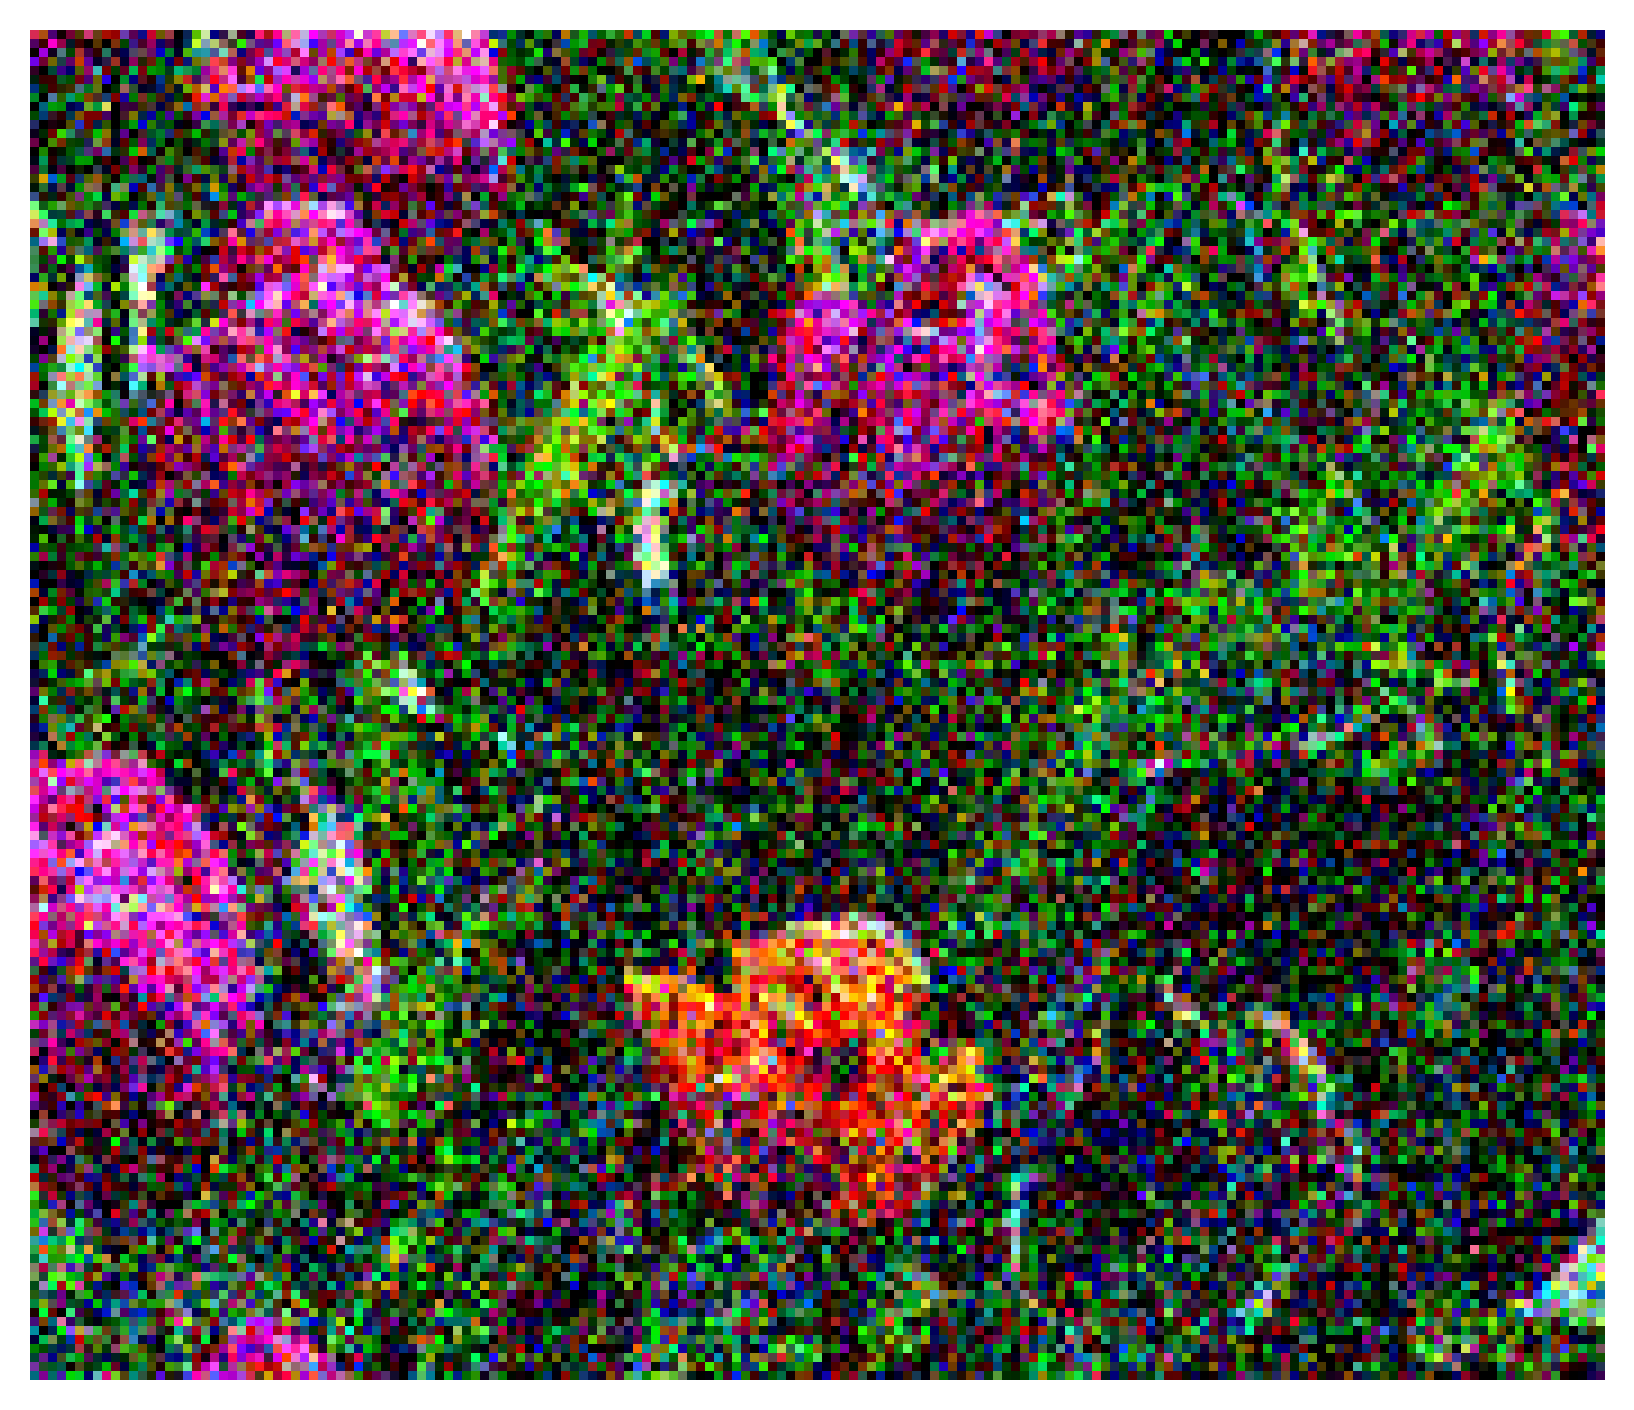
\includegraphics[width=\linewidth]{figs/q1b_zoomed_region1.png}
            \caption{}  % Caption for the upper right subfigure
            \label{fig:q1b_zoomed_bad}
        \end{subfigure}\\[1ex]  % Add some space between the subfigures
        \begin{subfigure}{\textwidth}
            \centering
            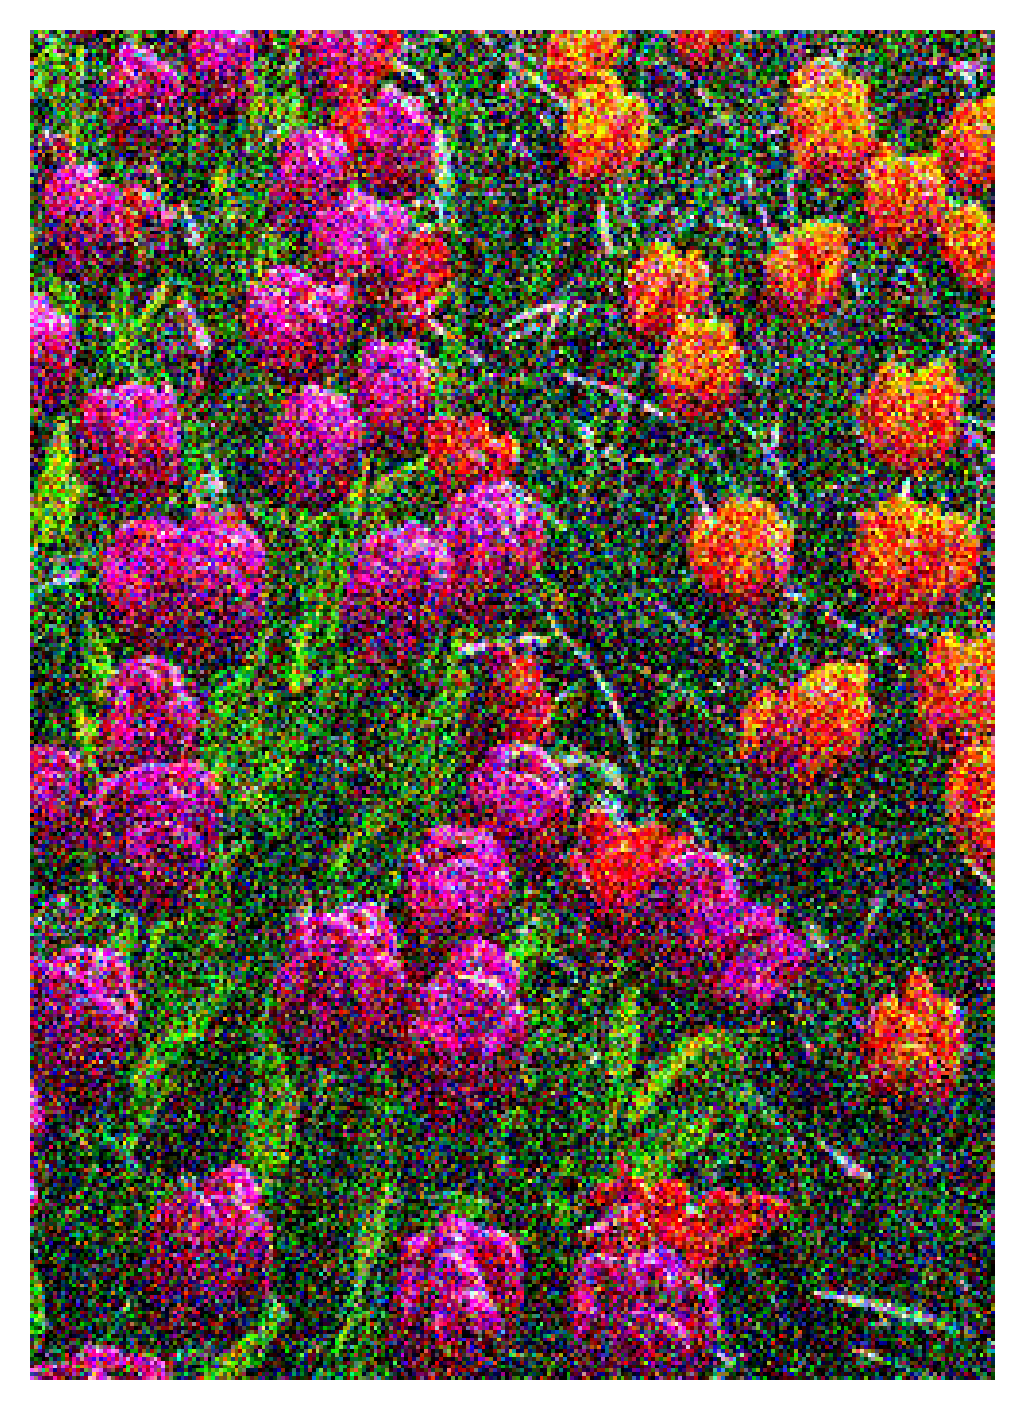
\includegraphics[width=\linewidth]{figs/q1b_zoomed_region2.png}
            \caption{}  % Caption for the lower right subfigure
            \label{fig:q1b_zoomed_bad2}
        \end{subfigure}
    \end{minipage}
    \caption{Zoomed in view of the segmentation: (a) Segmentation with bounding boxs around regions of interest where the segmentation has performed well, (b) Zoomed in view of the segmentation showing the exclusion of orange flower from the purple group, (c) Zoomed in view of the segmentation showing the exclusion of orange and red flowers that are occluded by flowers from the purple group.}
    \label{fig:flowers_seg_zoomed}
\end{figure}

\subsubsection{Discussion}
The main challenge in this segmentation is the segmentation of the purple flower heads that are in the foreground (closest to the camera). These flower heads have shadows on them, making the bottom half of the flower darker than the top half, making them difficult to fully segment with the current approach. An example such case is shown in figure \ref{fig:q1b_seg_lim}. This highlights the limitations of a segmentation algorithm which segments purely on colour. A potential improvement to this algorithm would be to consider spatial shape based information to better segment these flower heads or make use of more sophisticated pre-processing to remove the shadows.
% TODO: Make it clearer where the seg is failing, right now the masks are not showing in the zoomed regions so not obvious
\begin{figure}[H]
    \centering
    \begin{subfigure}{.8\textwidth}
        \centering
        \includegraphics[width=\linewidth]{figs/q1b_seg_w_bad_bbox.png}
        \caption{}  % Optional: add a specific caption here if needed.
        \label{fig:q1b_bad_seg_w_bbox}
    \end{subfigure}\\ % Add a line break to stack the next subfigure below
    \begin{subfigure}{.8\textwidth}
        \centering
        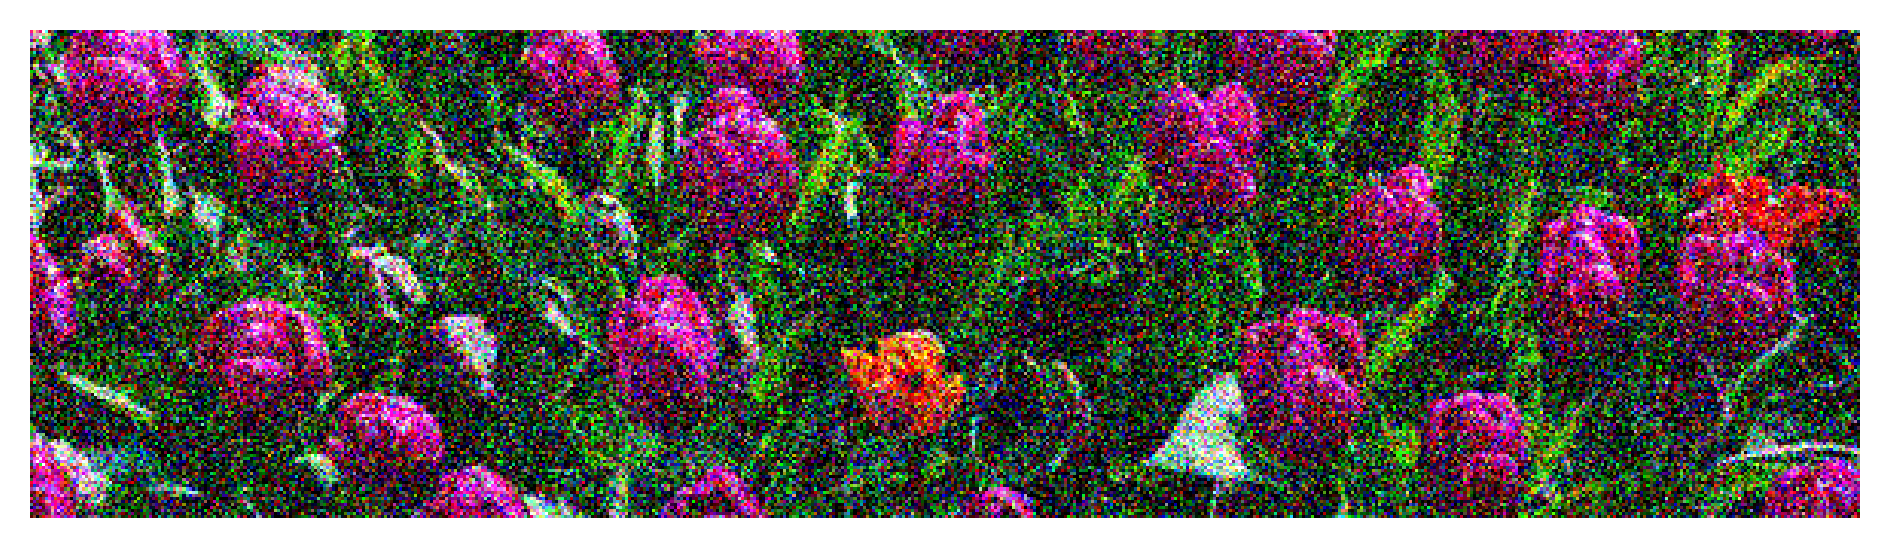
\includegraphics[width=\linewidth]{figs/q1b_bad_zoomed_region.png}
        \caption{}  % Optional: add a specific caption here if needed.
        \label{fig:q1b_bad_zoom}
    \end{subfigure}
    \caption{Limitations in segmentation of noisy flowers image: (a) Full view of the image with poorly segmented areas highlighted in a bounding box, demonstrating where the algorithm fails to accurately segment due to shadows. (b) Close-up view of a poorly segmented area, showing flower heads which feature strong shadows, impacting segmentation accuracy.}
    \label{fig:q1b_seg_lim}
\end{figure}

\subsection{Part C: Coin Image Segmentation}
This section details the segmentation algorithm of the coin image shown in Figure \ref{fig:coins_image}. The region to be segmented are the first coin in the first row, the second coin in the second row, the third coin in the third row and the fourth coin in the fourth row.
\begin{figure}[H]
    \centering
    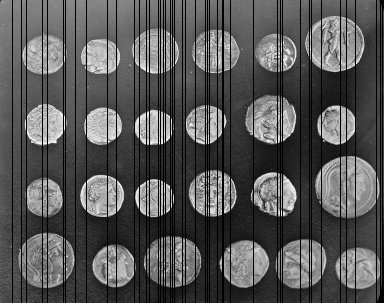
\includegraphics[width=0.5\textwidth]{../data/coins.png}
    \caption{Coin image.}
    \label{fig:coins_image}
\end{figure}

\subsubsection{Image Characteristics}
The image has been degraded with vertical line type artefacts. These artefacts have likely been synthetically generated and can be corrected by filtering. There is generally good contrast between the coins and the background, however fig \ref{fig:otsu_threshold_coins}, applying an otsu threshold reveals that the coins in the first row are not clearly separated from the background. Edge detection to segment the coins is likely to perform better in this case.

\begin{figure}[H]
    \centering
    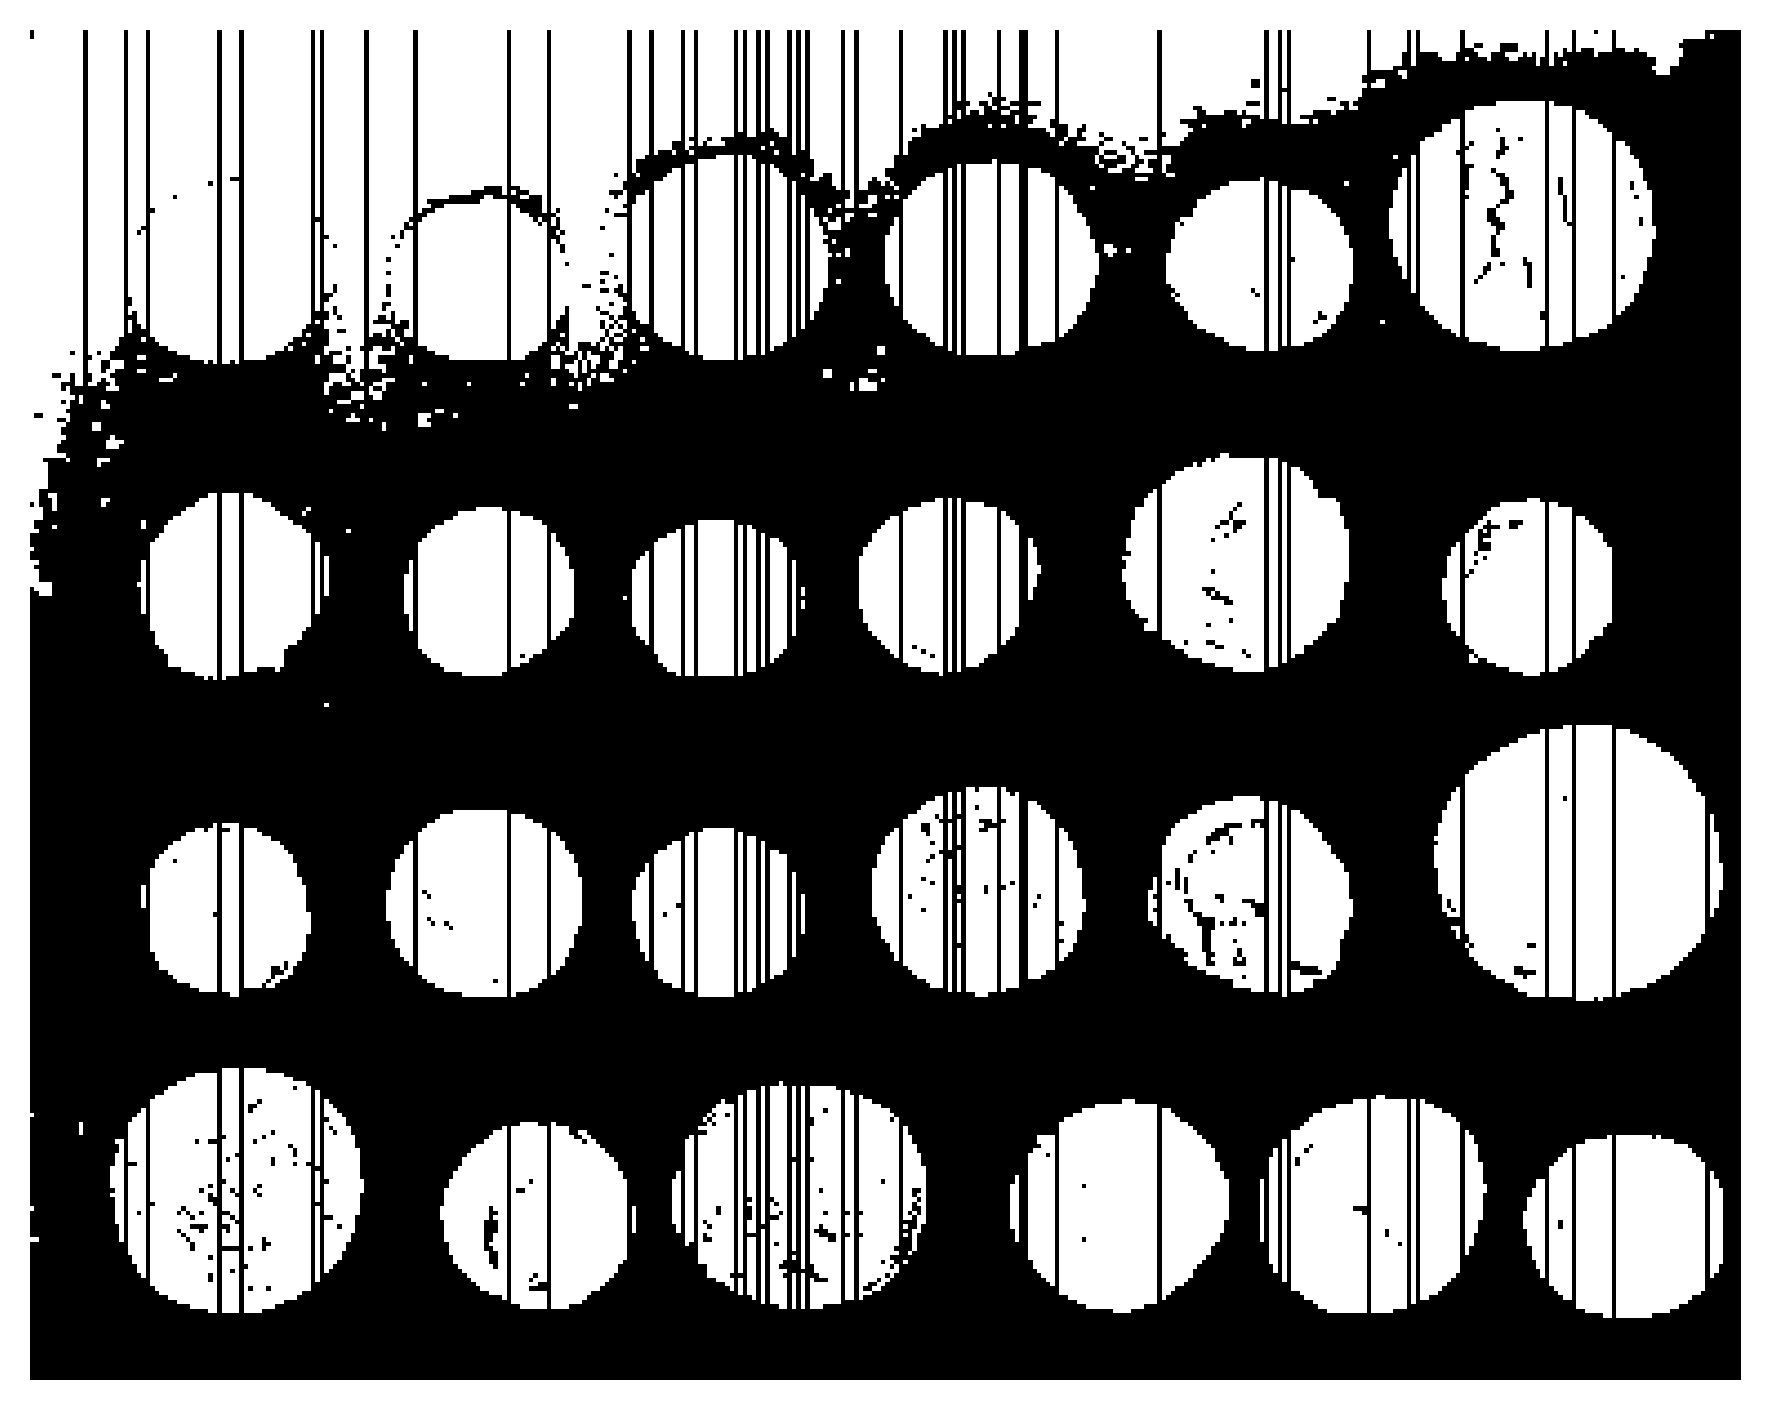
\includegraphics[width=0.5\textwidth]{figs/q1c_otsu_thresholded.png}  % Replace with your image file
    \caption{Effect of Otsu thresholding on the coin image.}
    \label{fig:otsu_threshold_coins}
\end{figure}

\subsubsection{Assumptions}
To select the required coins for the task, the algorithm assumes that the coins are arranged in 4 rows with 6 columns, without making prior assumptions on what coin belongs to which position in the grid. The algorithm also assumes that the coins are not touching each other. Lastly, it assumes that the background is the largest connected component in the image.
\subsubsection{Segmentation Algorithm}

\begin{itemize}
\item \textbf{Row-wise Median Filtering:} Initially, a row-wise median filter is applied to the image to remove vertical line artefacts. This step is crucial to recover high quality edges for subsequent edge detection.
\item \textbf{Edge Detection with Canny:} Canny edge detection is a multi-stage algorithm that uses Gaussian smoothing to reduce noise, then detects edges by identifying areas with high gradient magnitudes. It employs a double threshold to classify edges into strong, weak, and non-edges: strong edges exceed the high threshold and are confirmed as true edges; weak edges between the two thresholds are only confirmed if connected to strong edges; and areas below the low threshold are dismissed as non-edges. This method ensures robust edge continuity and noise suppression.
\item \textbf{Dilation of Edges:} After detecting edges, a dilation operation is performed using an elliptical structuring element. This step helps to close small gaps in the detected edges, which aids in forming continuous outlines for the coins.
\item \textbf{Removal of the Largest Component:} The resulting image is then inverted and connected components are labelled. The largest connected component is assumed to be the background and is removed.
\item \textbf{Integration of Edges and Mask:} Edges detected from the Canny step are added to the mask of coins to enhance the definitions of the coins' borders and 'close' the coins so that the mask is more faithful to the actual coin shapes.
\item \textbf{Binary Hole Filling:} A binary hole filling operation is then performed to fill any unsegmented areas within each coin. 
\item \textbf{Median Filtering on Mask:} Finally, to remove spurious regions of the mask which arose from edges that did not belong to any coins, both row-wise and column-wise median filtering is applied to the mask. This step removes regions that are not part of the coins. This step ensures that the next step of removing small components need not require too large a threshold, risking the removal of actual coins.
\item \textbf{Removal of Small Connected Components:} Finally, any small connected components with an area less than 100 pixels are removed from the mask. This step ensures that only the coins are retained in the final mask.
\item \textbf{Sorting and Assigning Grid Positions:} The centroids of the coin masks are then sorted based on their vertical and horizontal coordinates to assign each coin a grid position. 
\item \textbf{Selecting Specific Coins:} The coins whose grid position matches the required positions are selected.

\end{itemize}

\begin{figure}[H]
    \centering
    \begin{subfigure}{.33\textwidth}
        \centering
        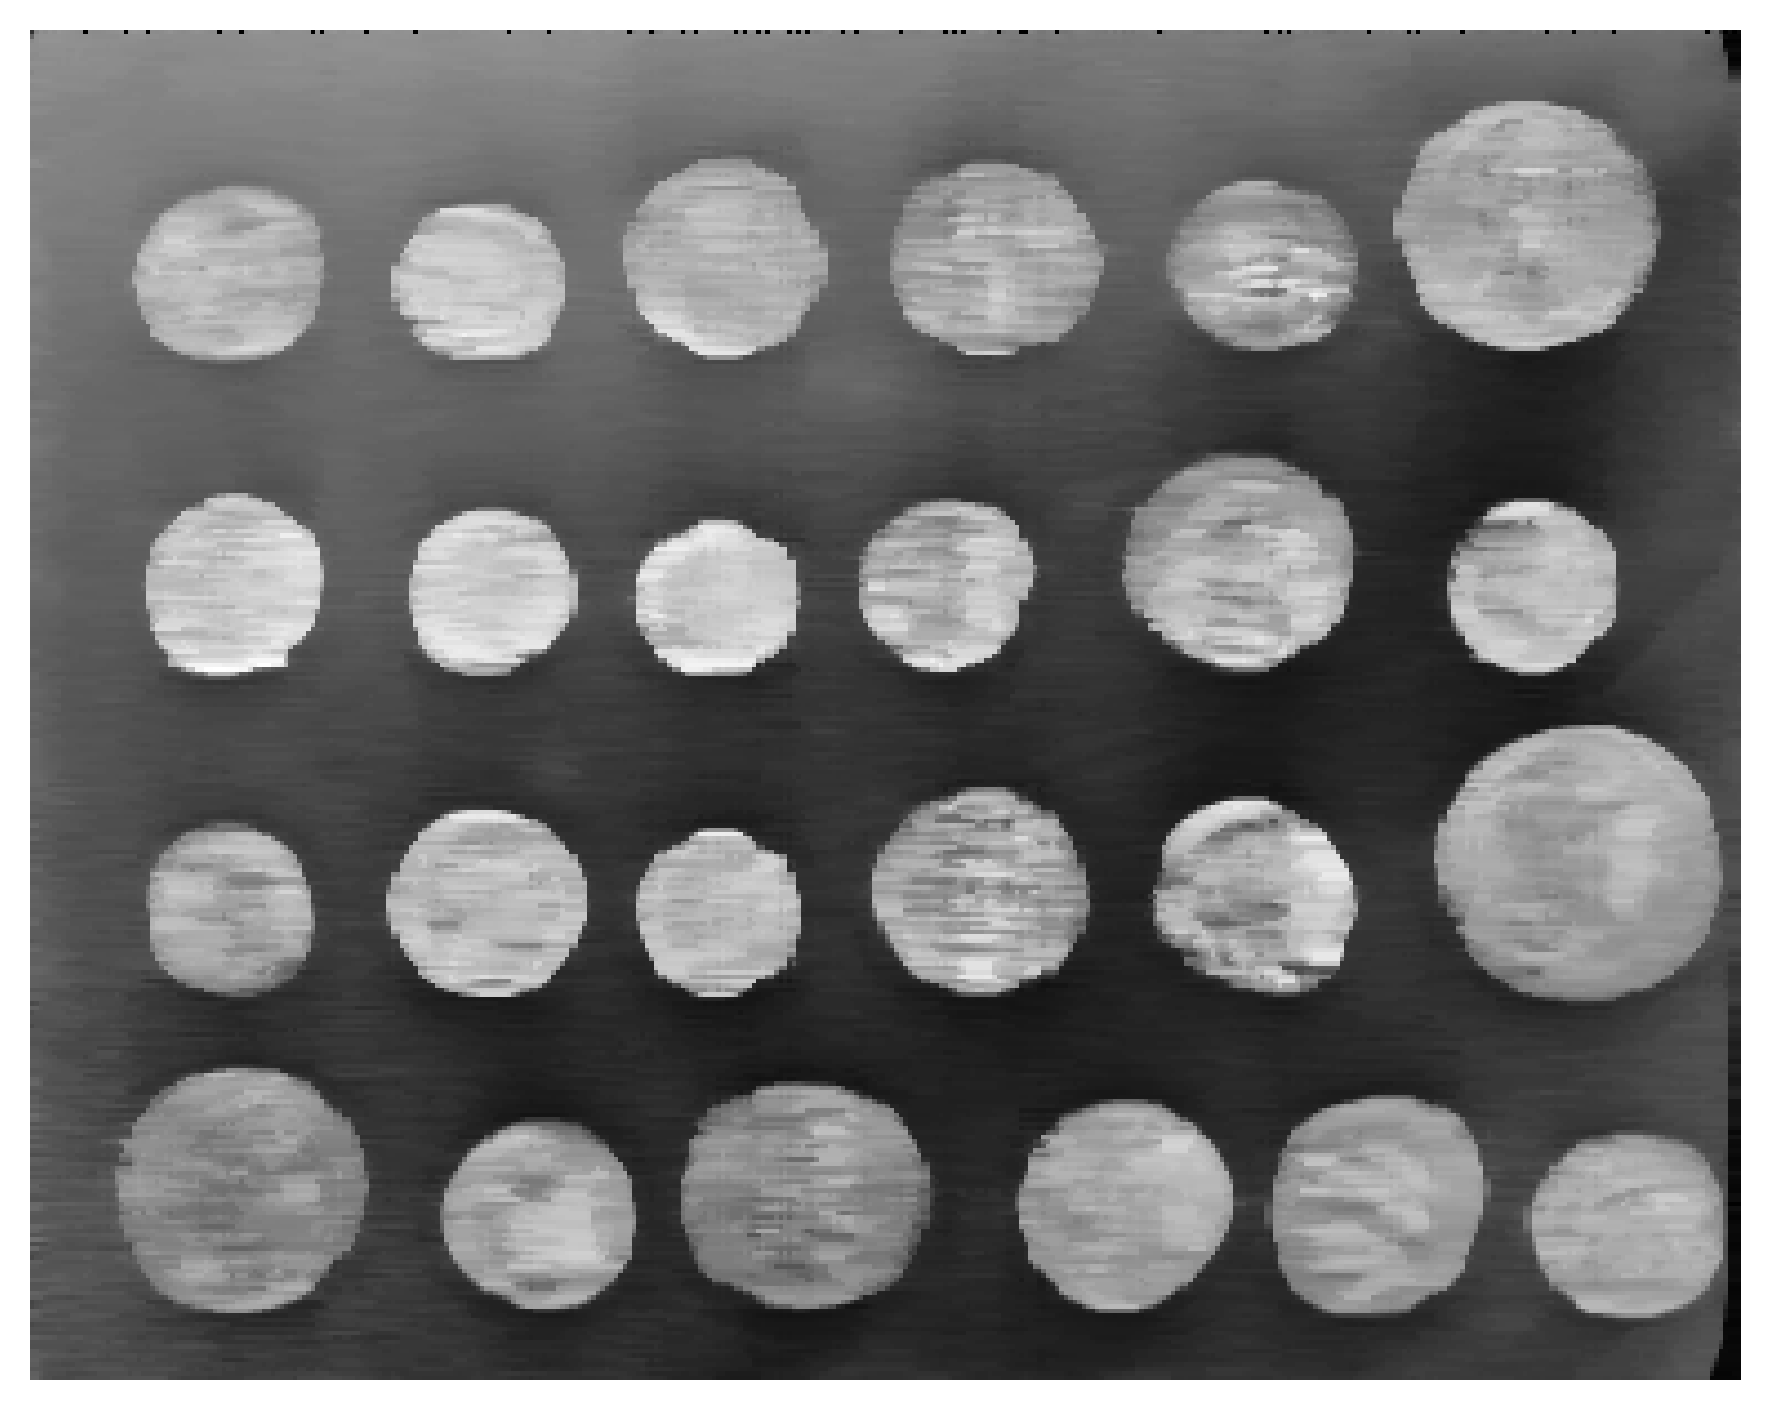
\includegraphics[width=\linewidth]{figs/q1c_init_median_filtered.png}
        \caption{}
    \end{subfigure}%
    \begin{subfigure}{.33\textwidth}
        \centering
        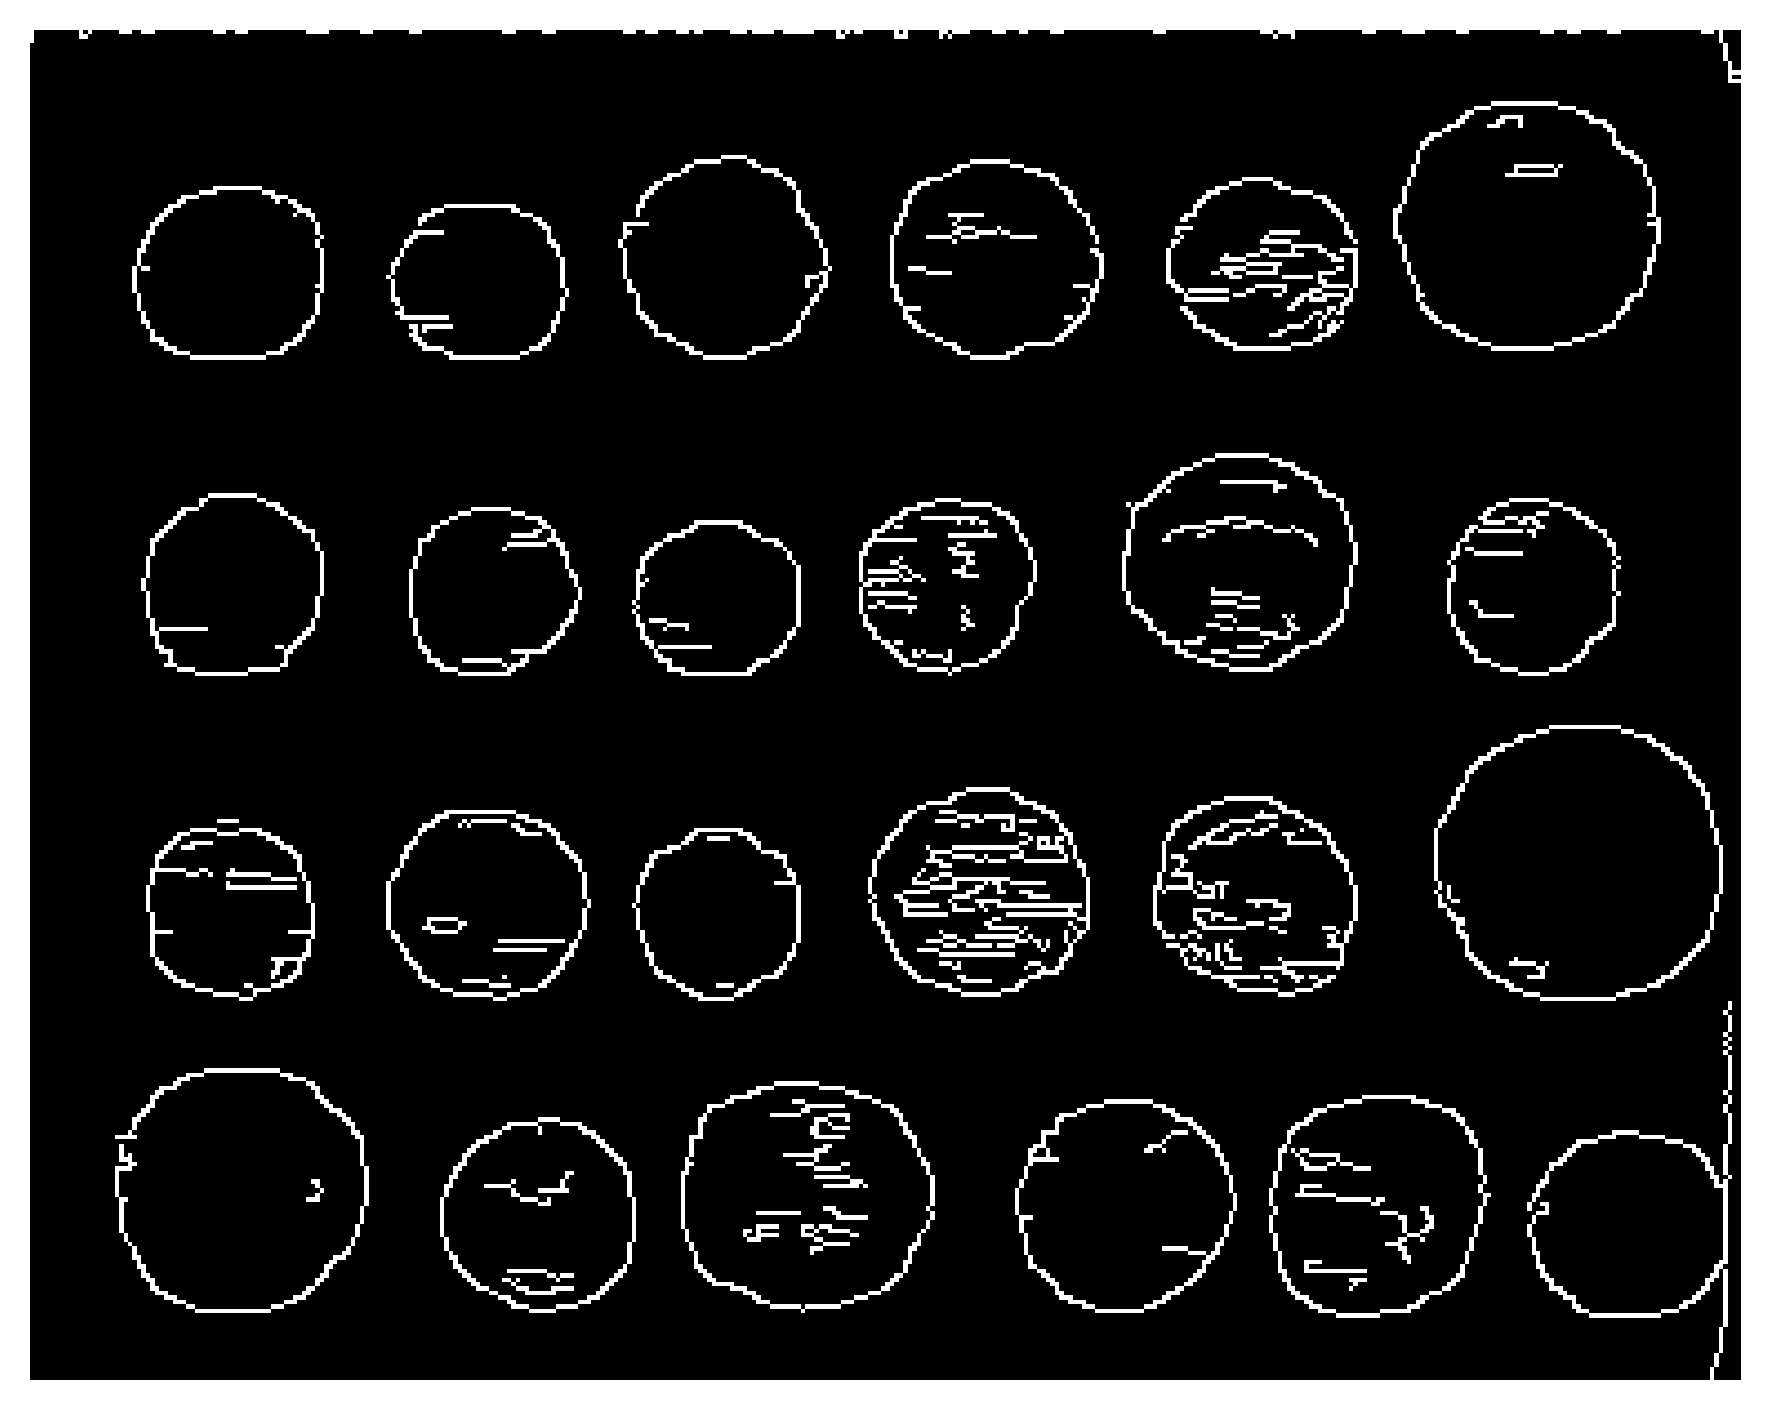
\includegraphics[width=\linewidth]{figs/q1c_canny_edges.png}
        \caption{}
    \end{subfigure}%
    \begin{subfigure}{.33\textwidth}
        \centering
        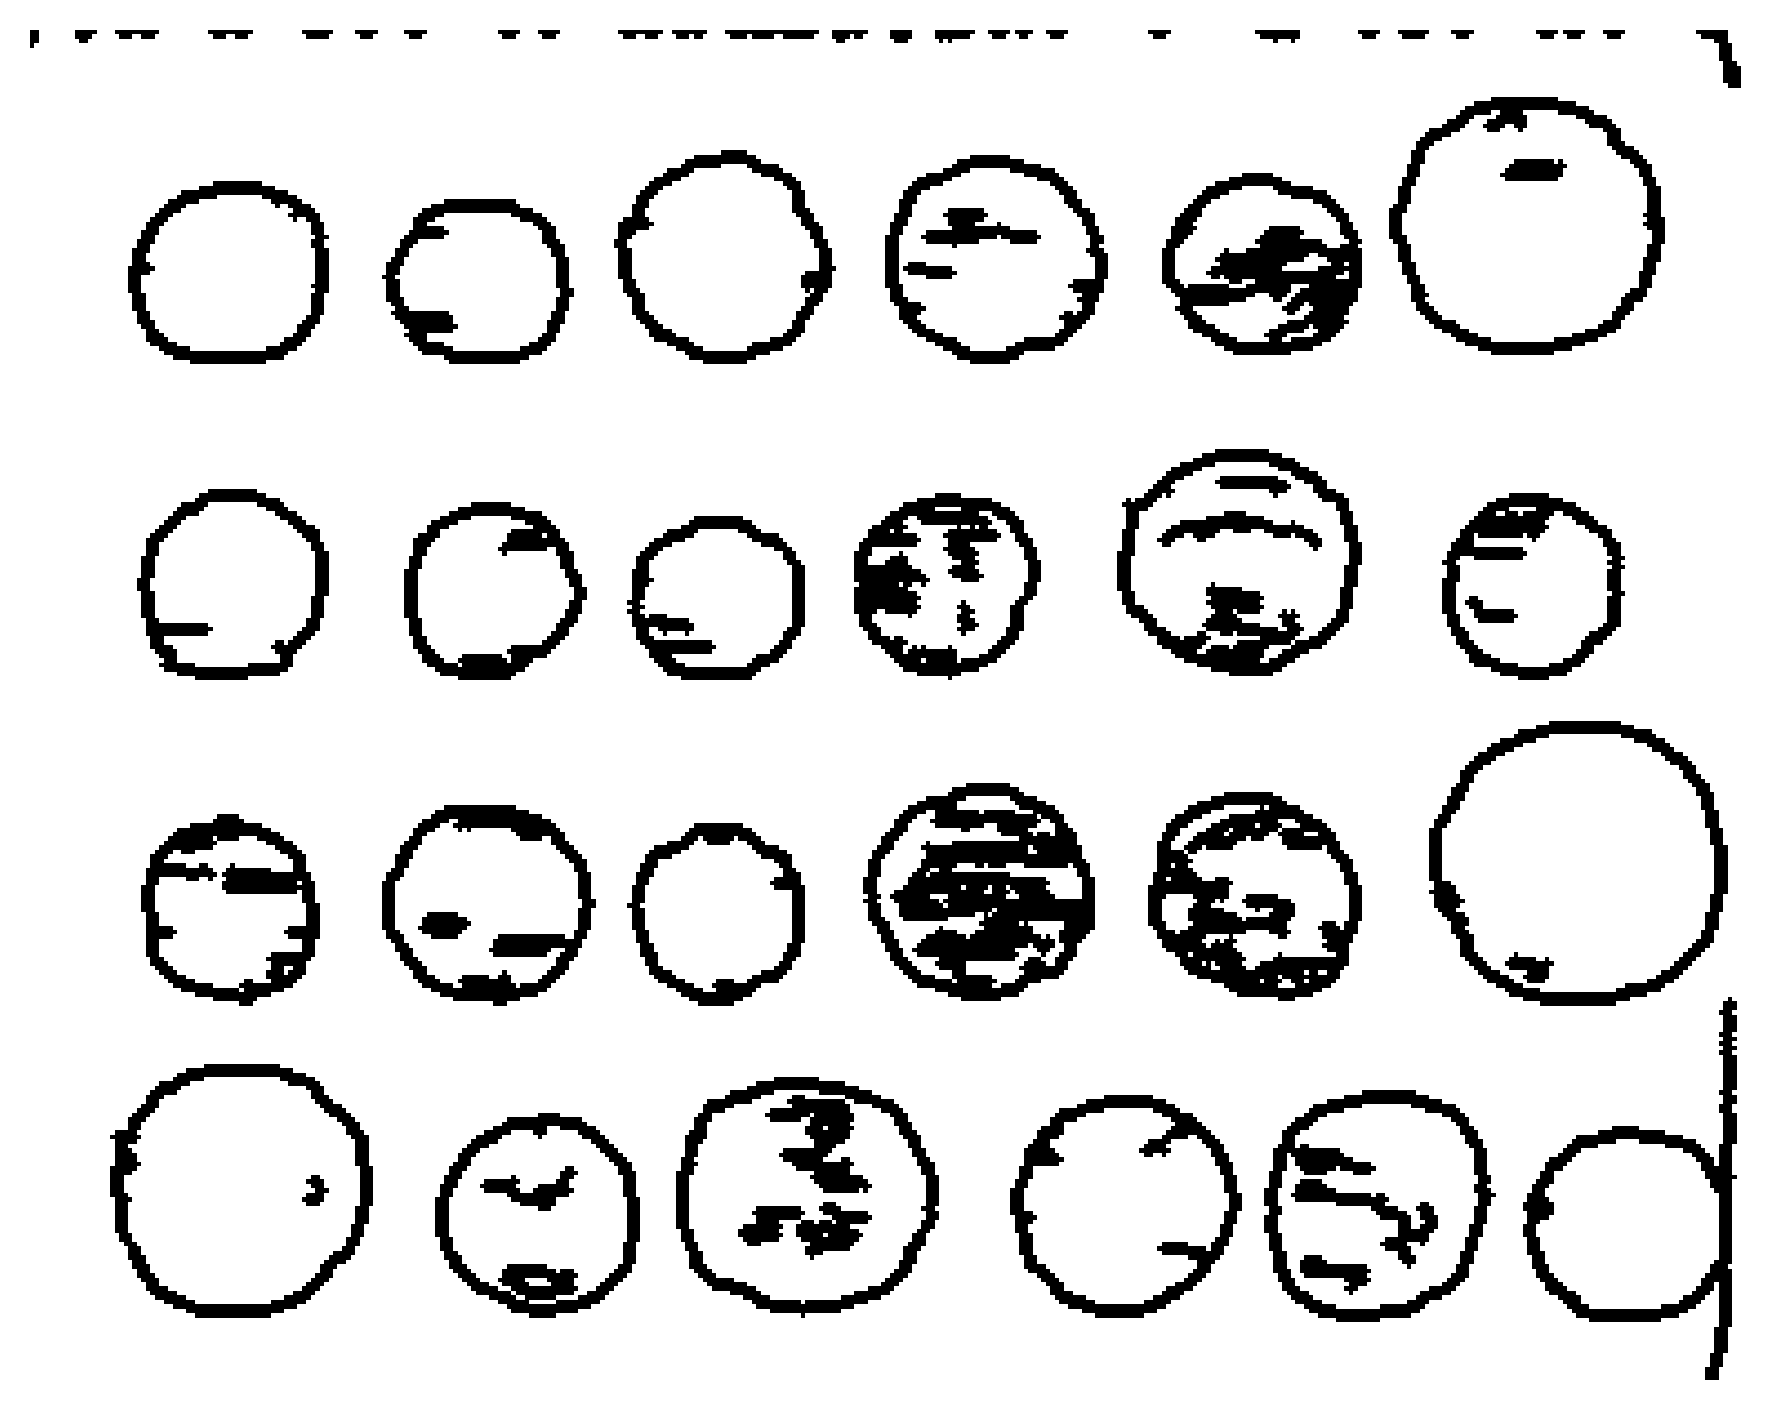
\includegraphics[width=\linewidth]{figs/q1c_dilated_inverted_edges.png}
        \caption{}
    \end{subfigure}%

    \begin{subfigure}{.33\textwidth}
        \centering
        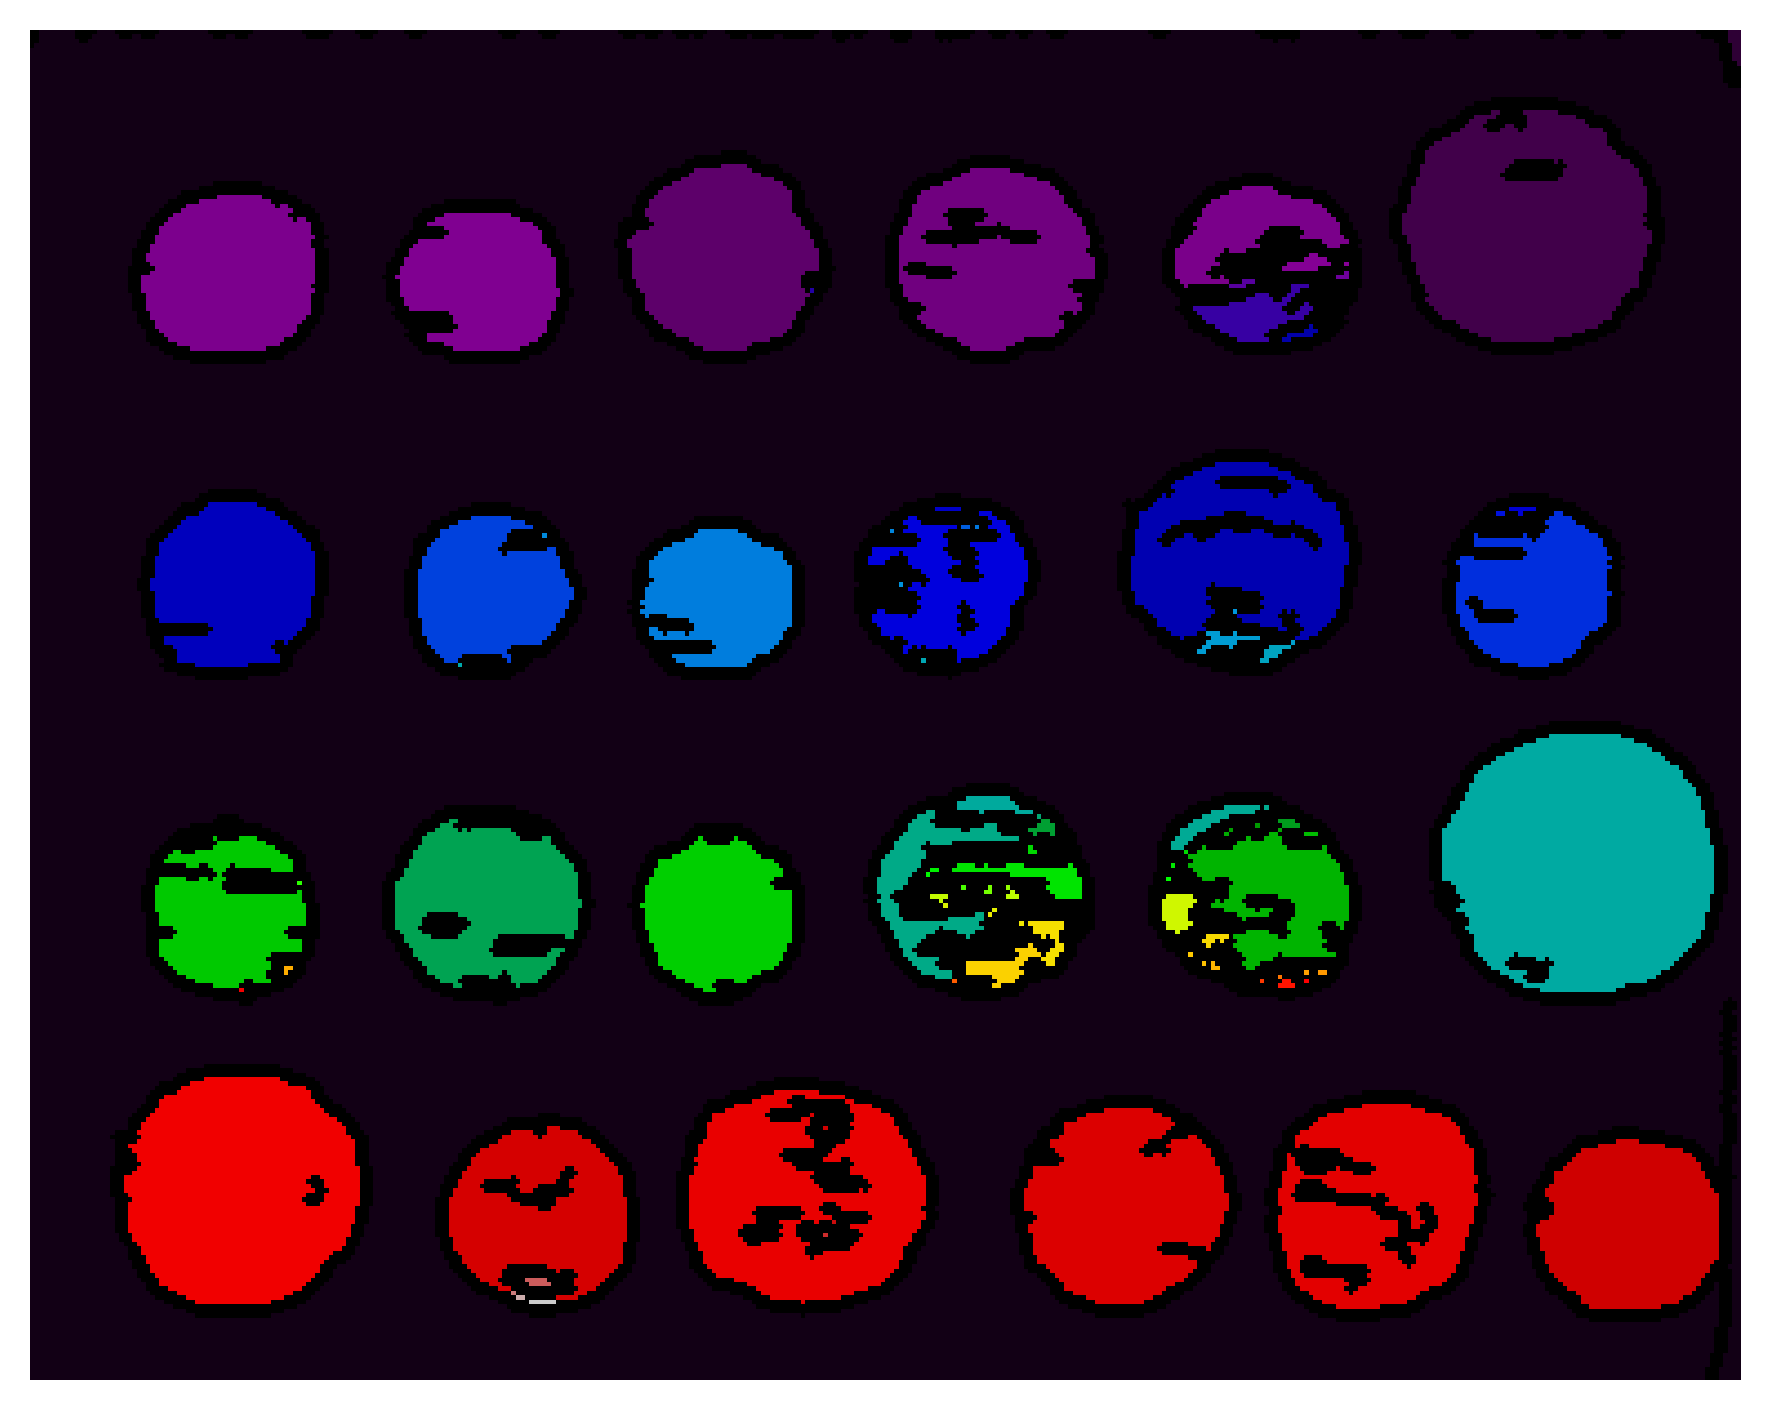
\includegraphics[width=\linewidth]{figs/q1c_connected_components.png}
        \caption{}
    \end{subfigure}%
    \begin{subfigure}{.33\textwidth}
        \centering
        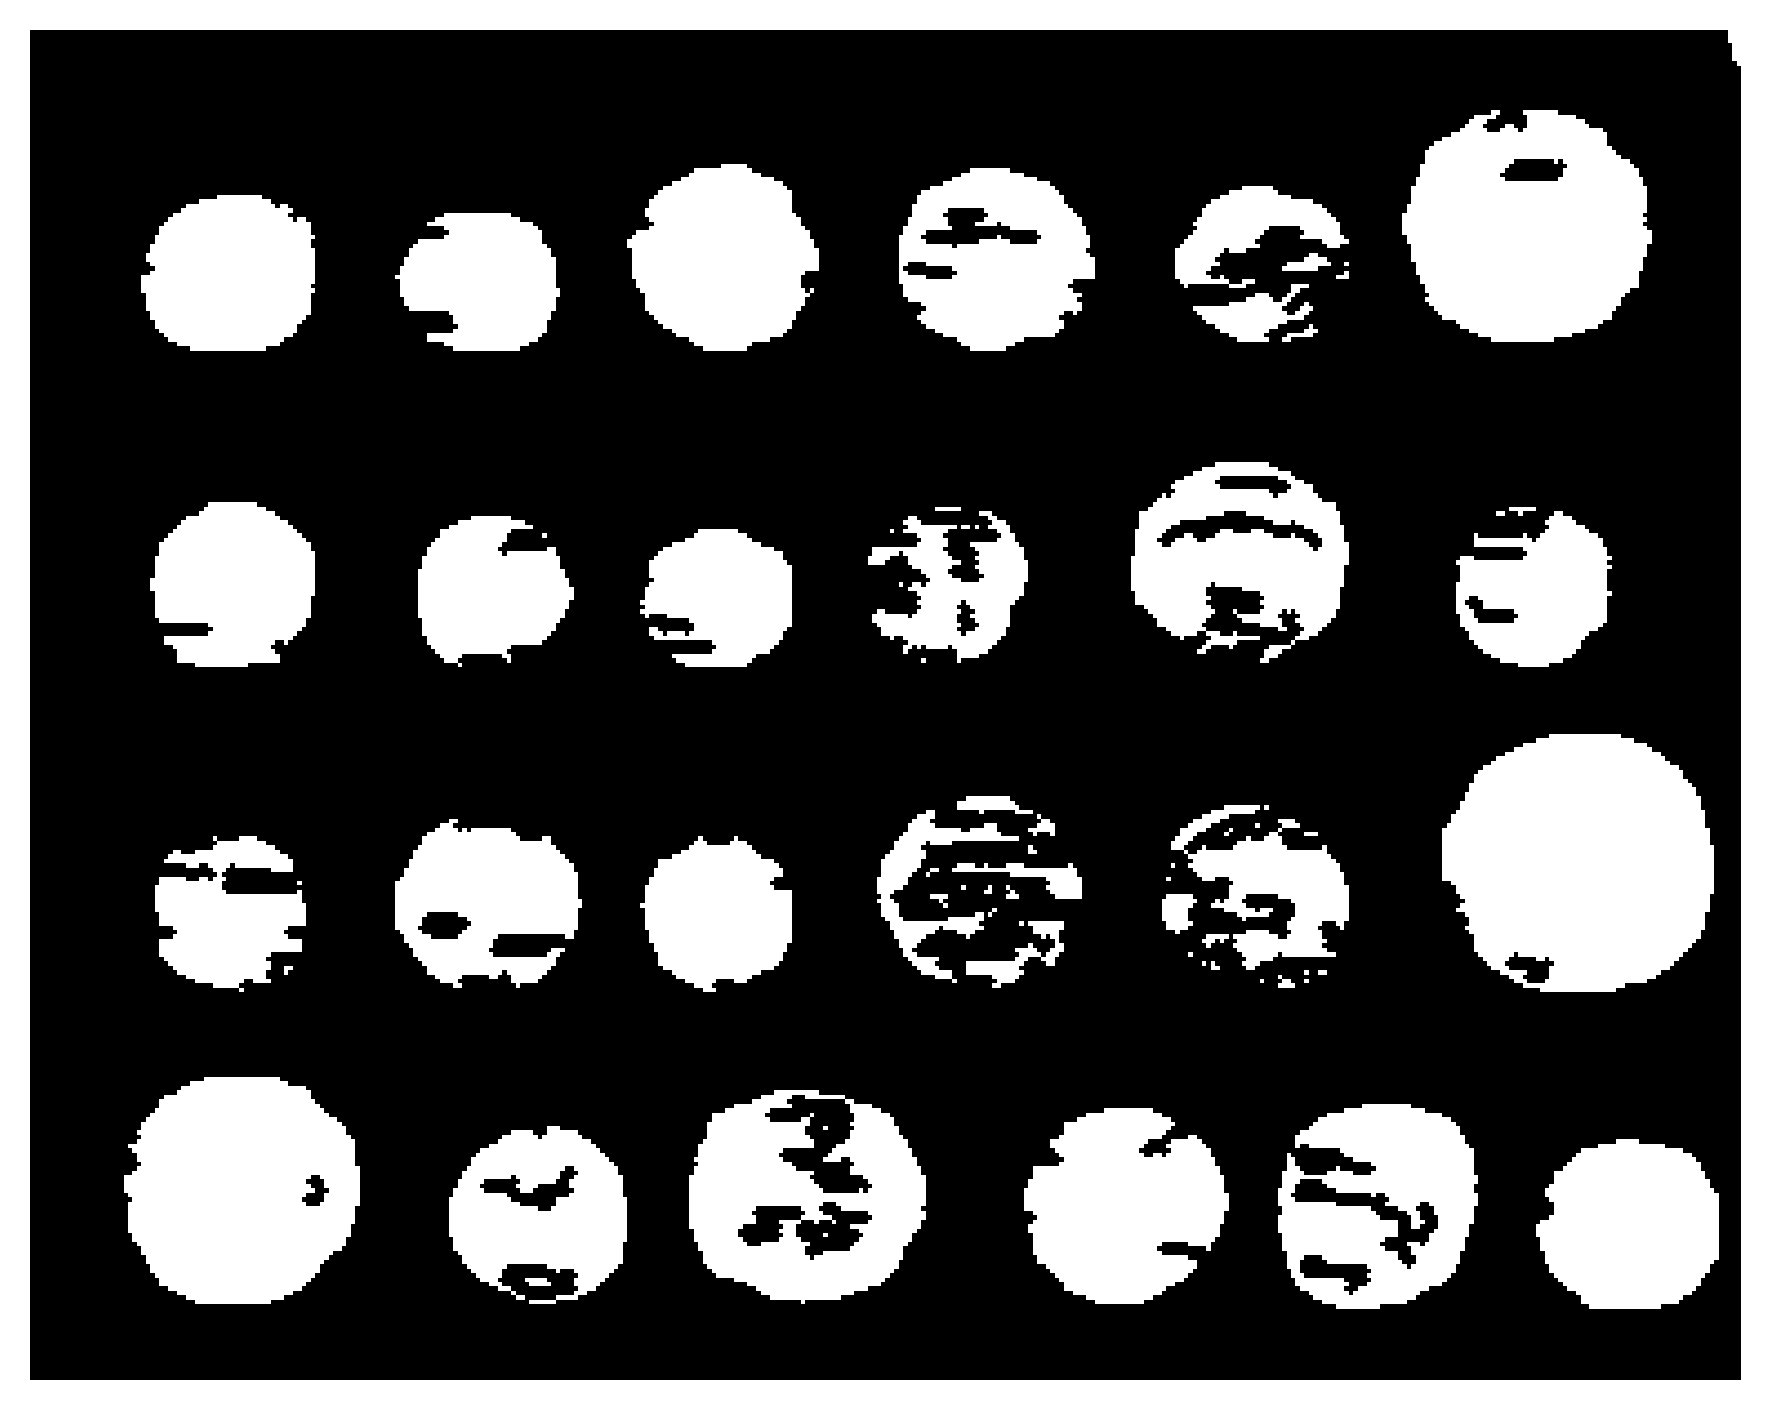
\includegraphics[width=\linewidth]{figs/q1c_mask_no_bg.png}
        \caption{}
    \end{subfigure}%
    \begin{subfigure}{.33\textwidth}
        \centering
        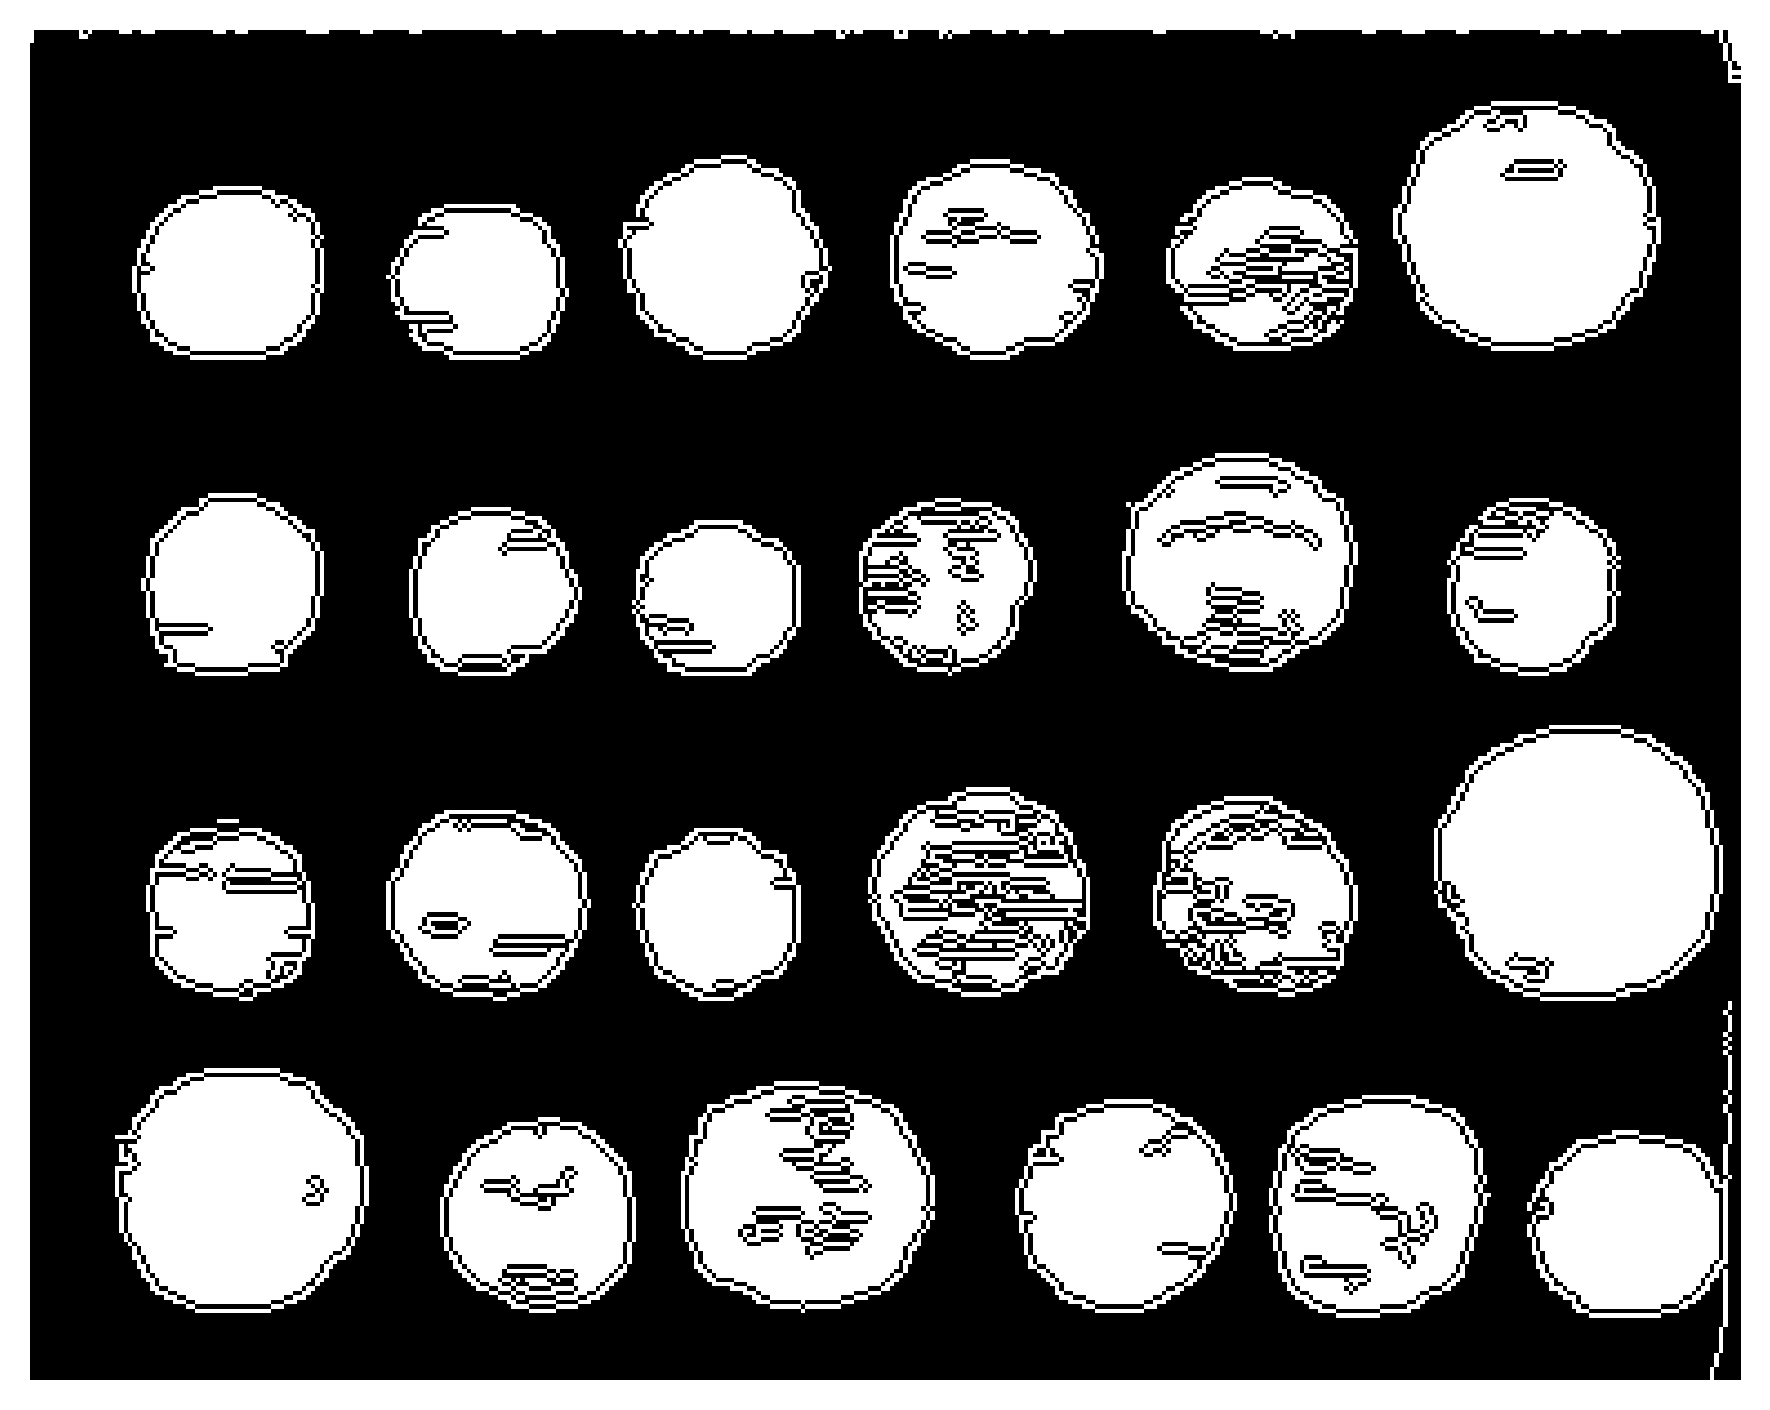
\includegraphics[width=\linewidth]{figs/q1c_mask_edges.png}
        \caption{}
    \end{subfigure}%

    \begin{subfigure}{.33\textwidth}
        \centering
        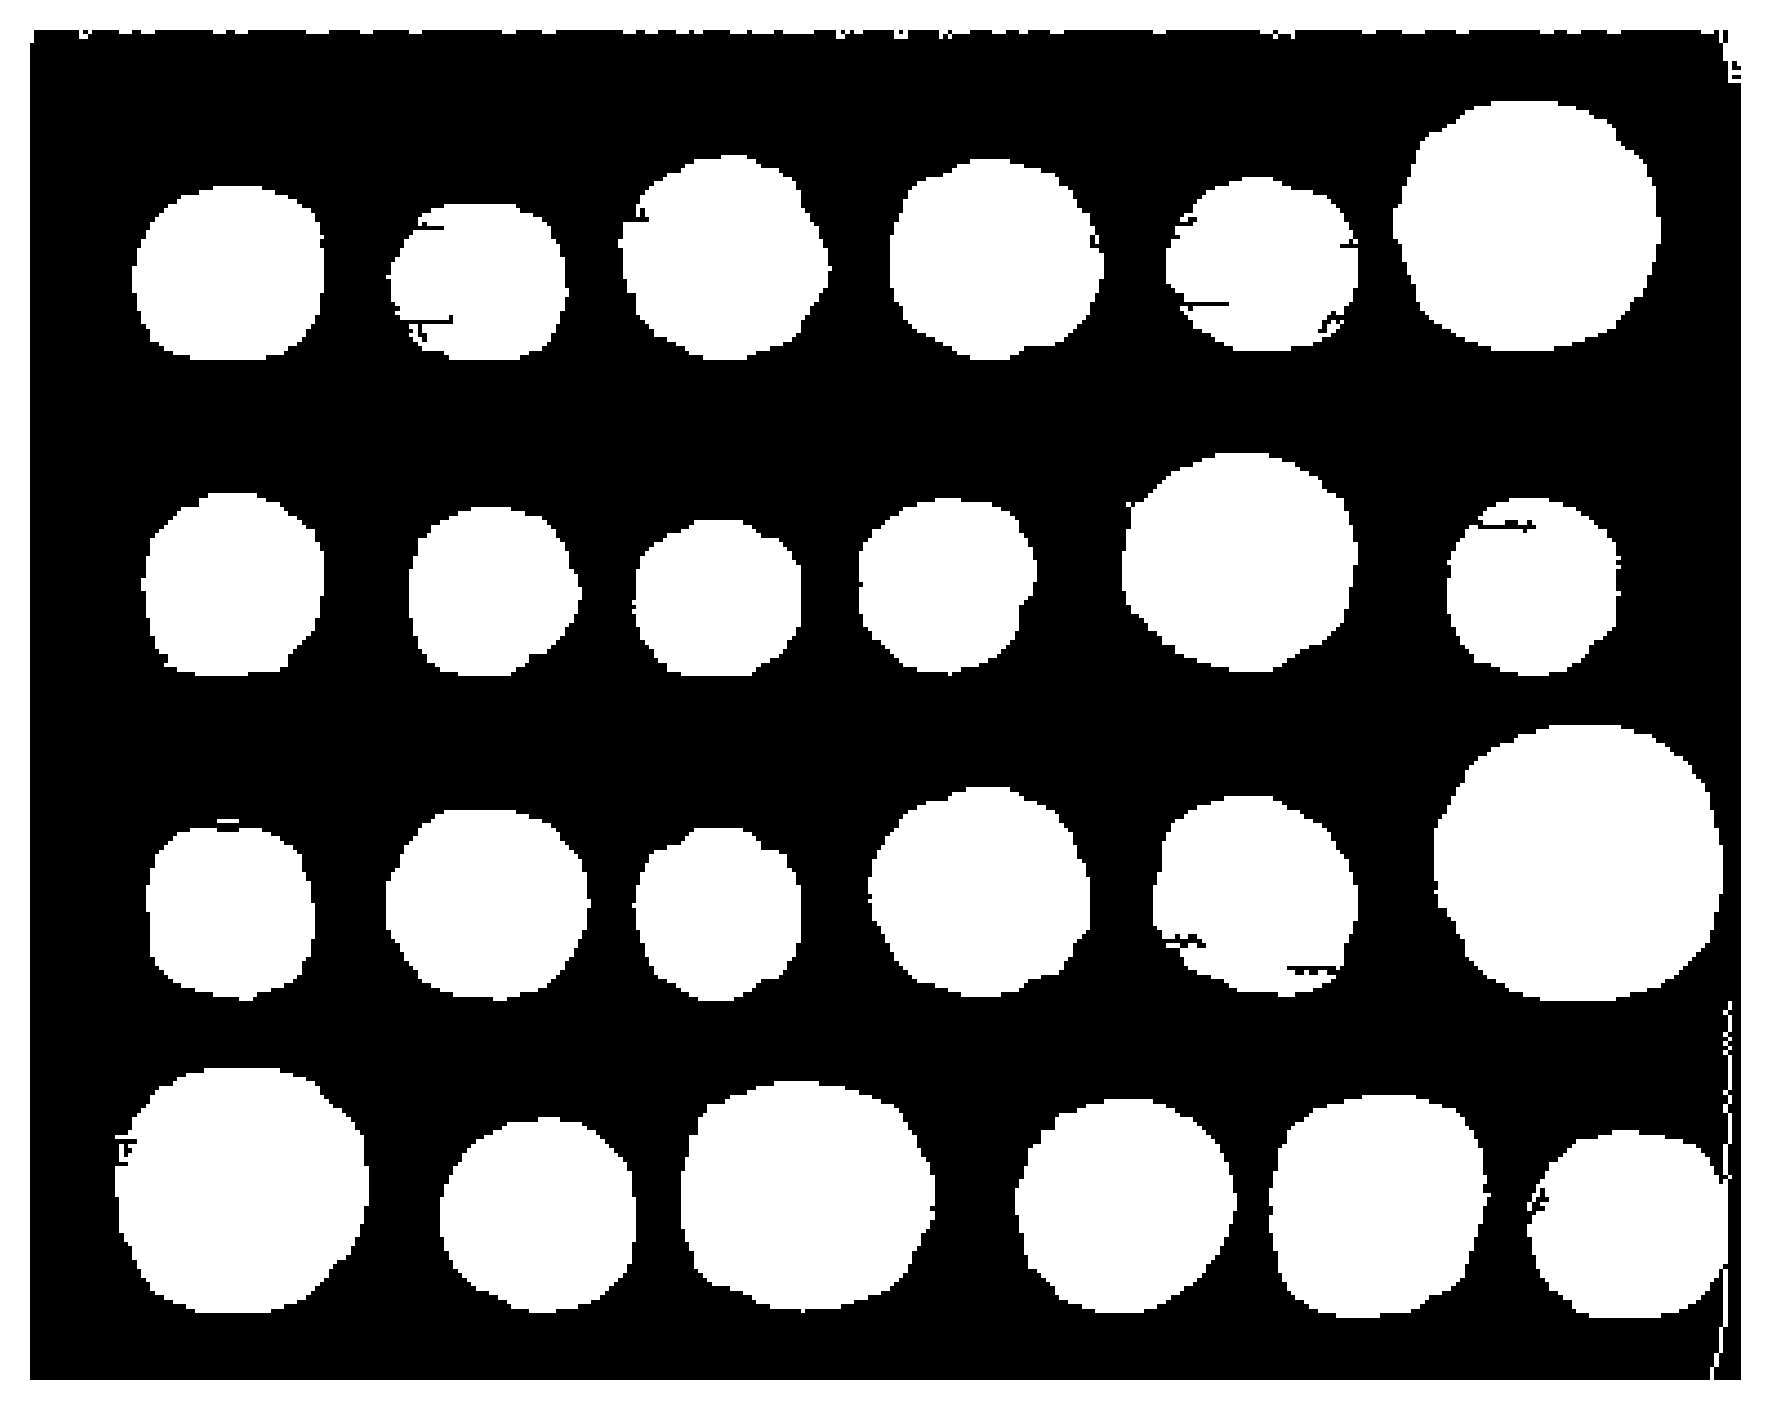
\includegraphics[width=\linewidth]{figs/q1c_binary_hole_filled.png}
        \caption{}
    \end{subfigure}%
    \begin{subfigure}{.33\textwidth}
        \centering
        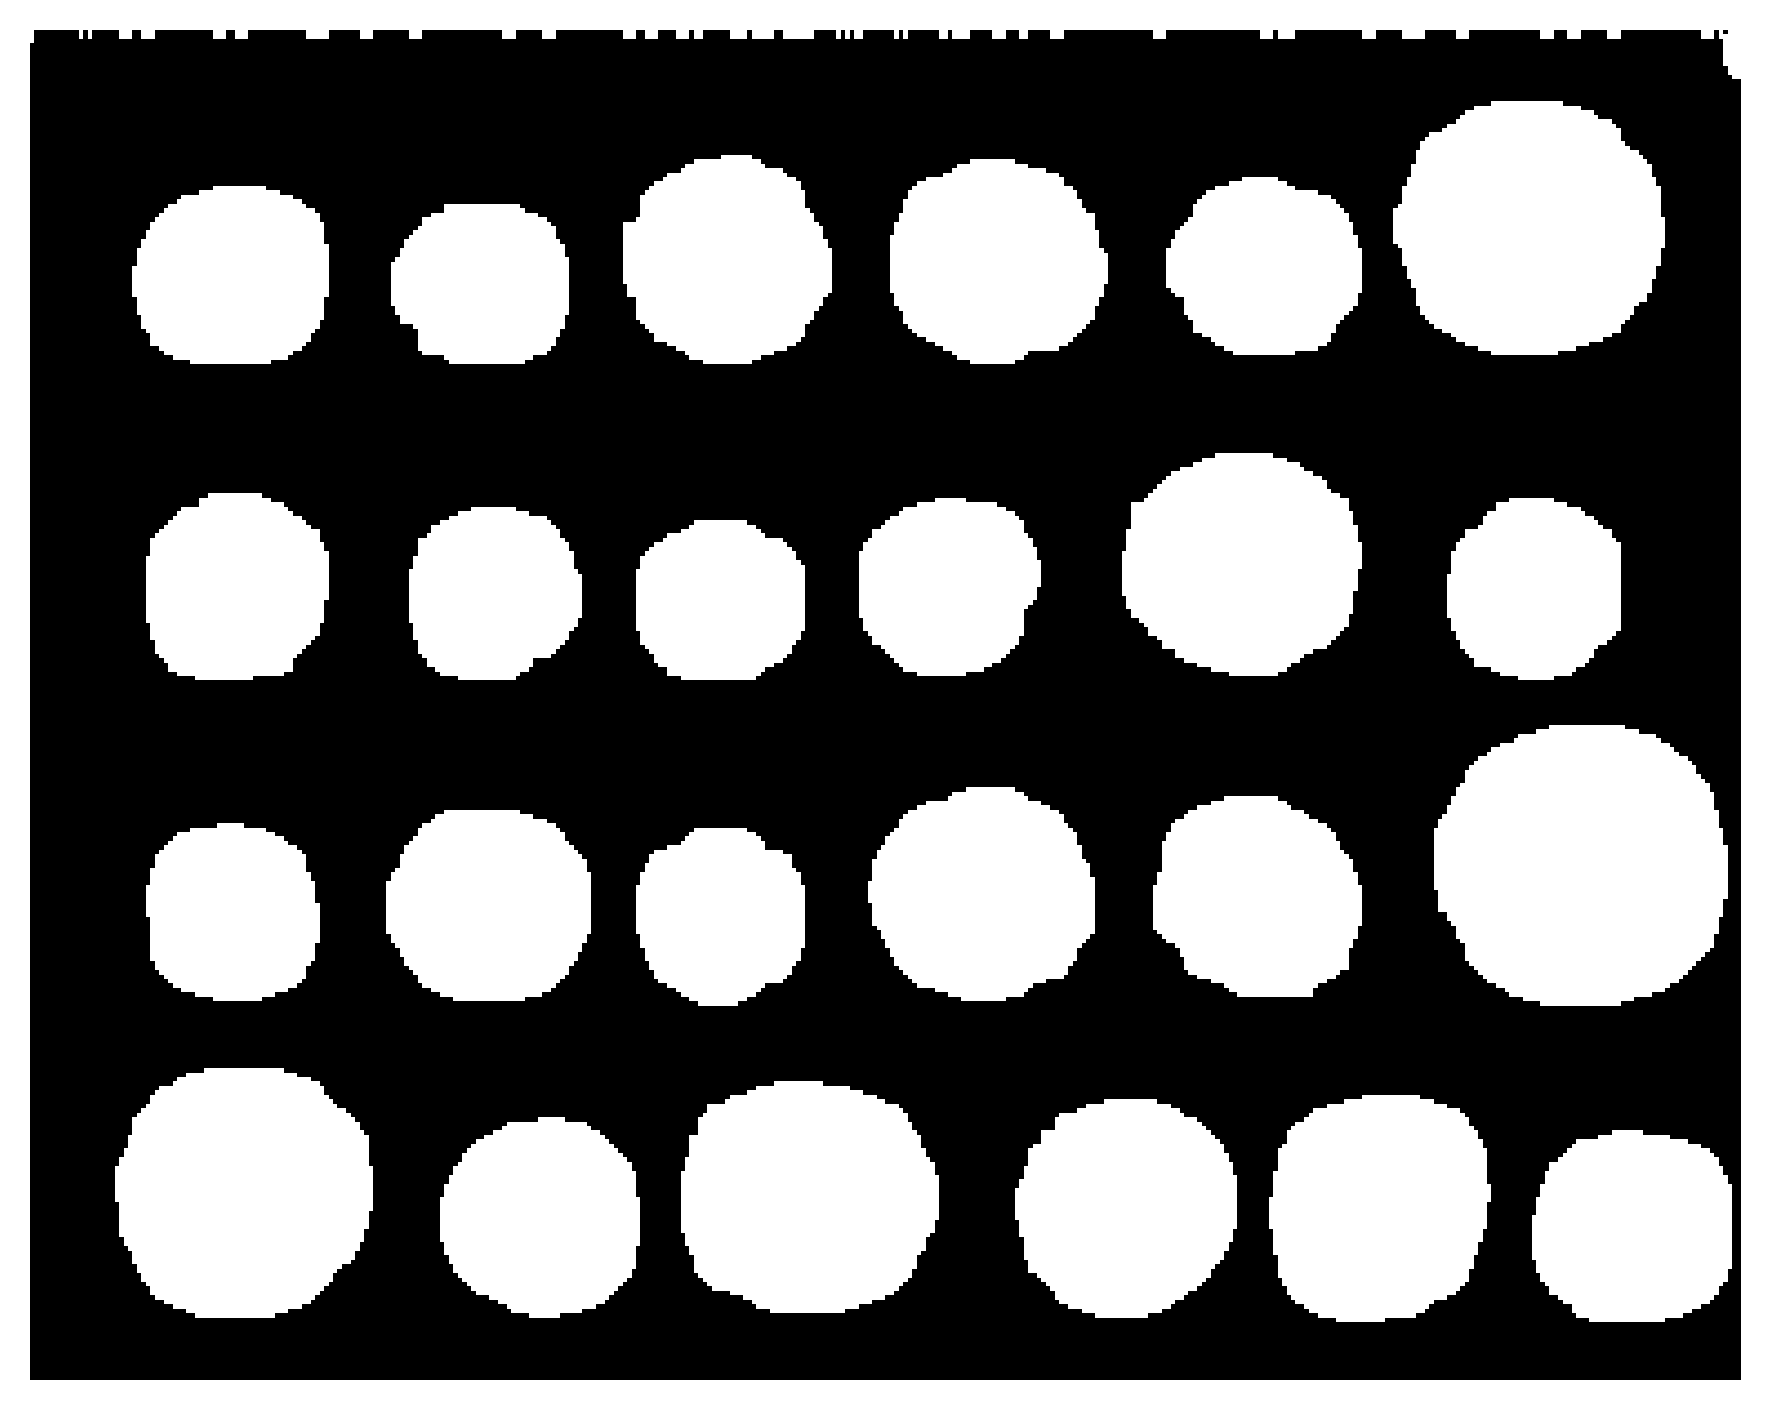
\includegraphics[width=\linewidth]{figs/q1c_median_filtered_mask.png}
        \caption{}
    \end{subfigure}%
    \begin{subfigure}{.33\textwidth}
        \centering
        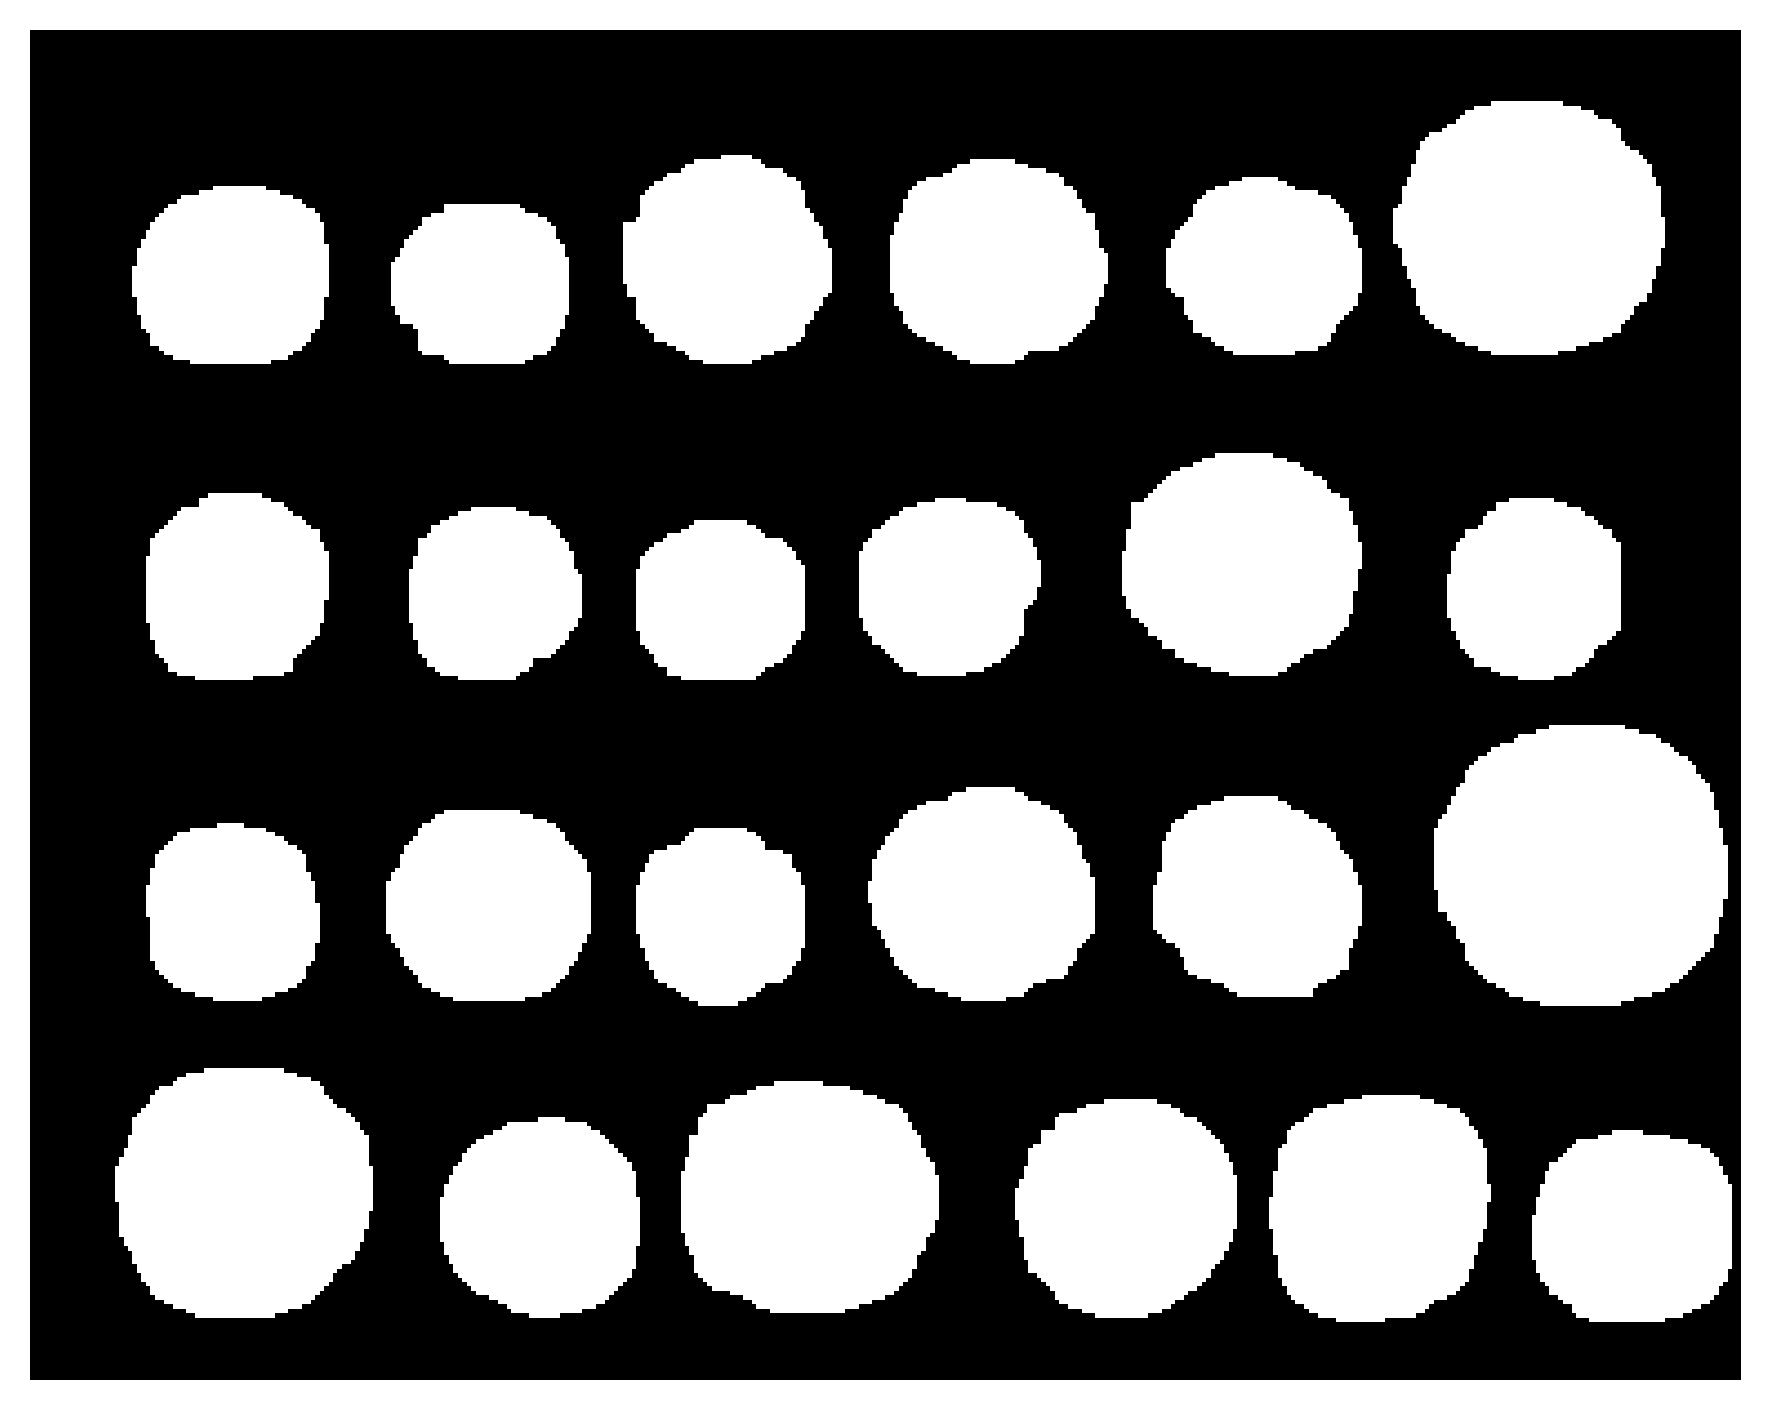
\includegraphics[width=\linewidth]{figs/q1c_mask_no_small_components.png}
        \caption{}
    \end{subfigure}%

    \begin{subfigure}{.45\textwidth}
        \centering
        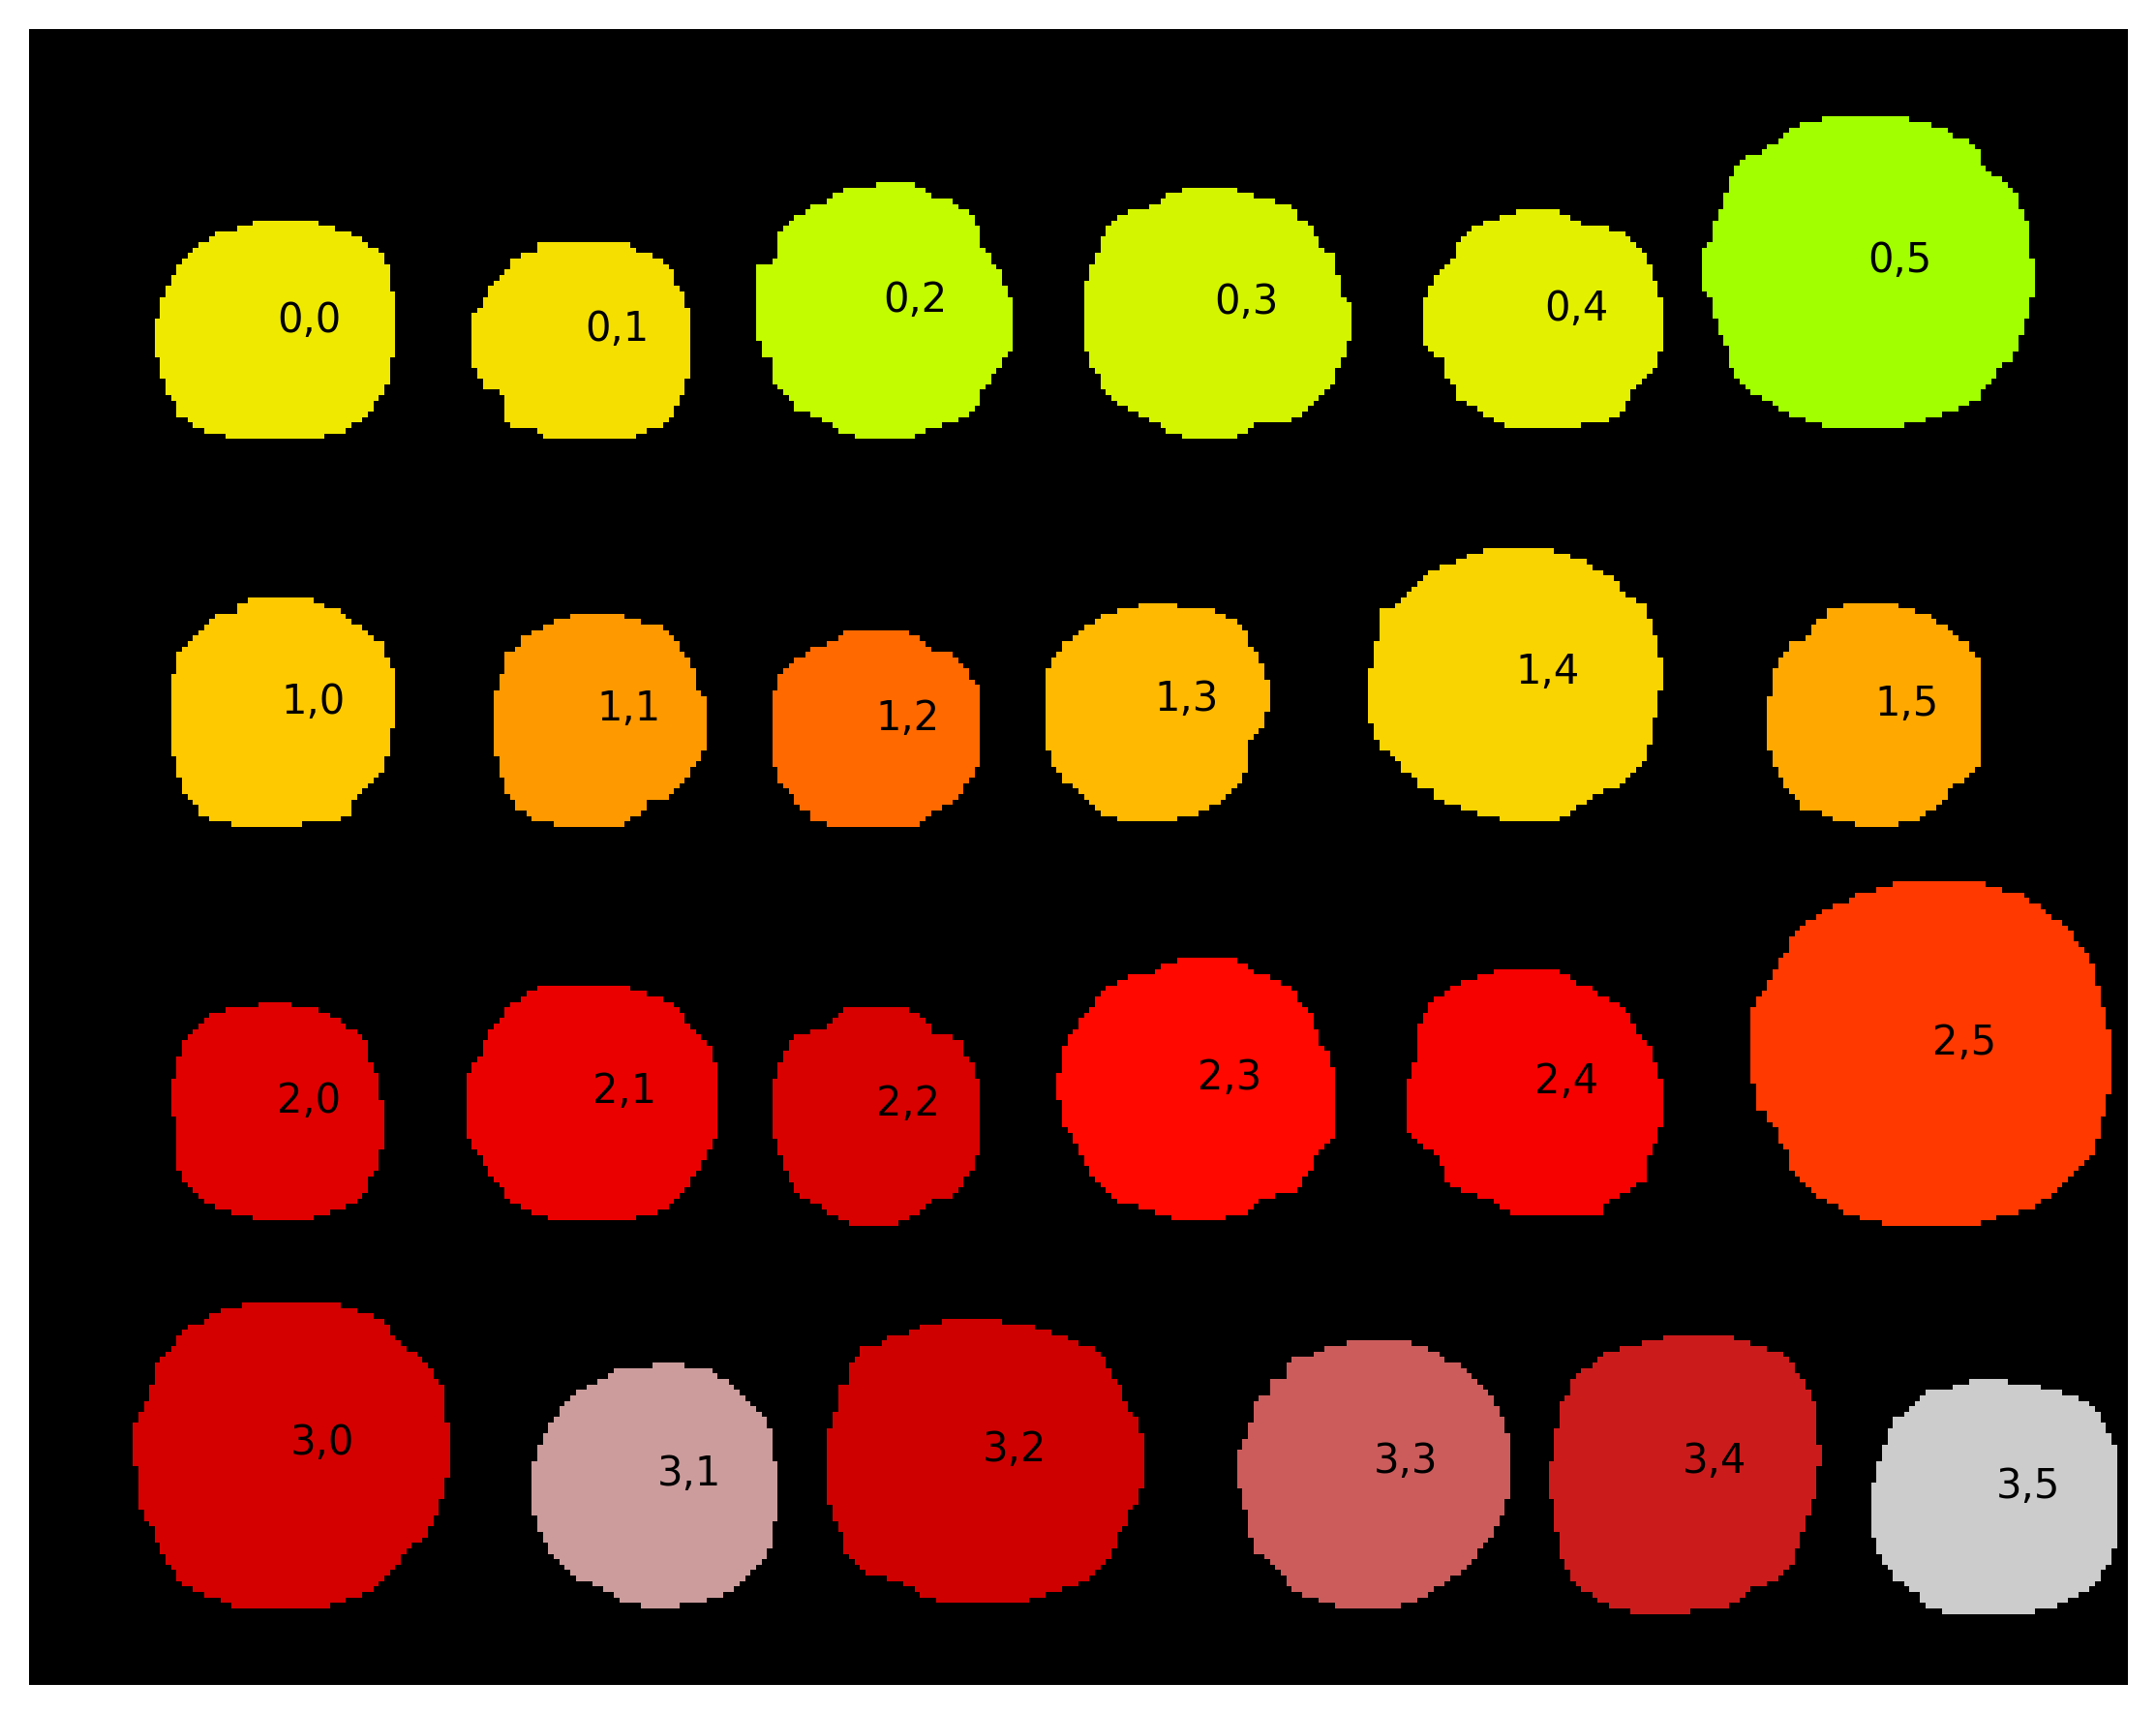
\includegraphics[width=\linewidth]{figs/q1c_identified_coins.png}
        \caption{}
    \end{subfigure}%
    \begin{subfigure}{.45\textwidth}
        \centering
        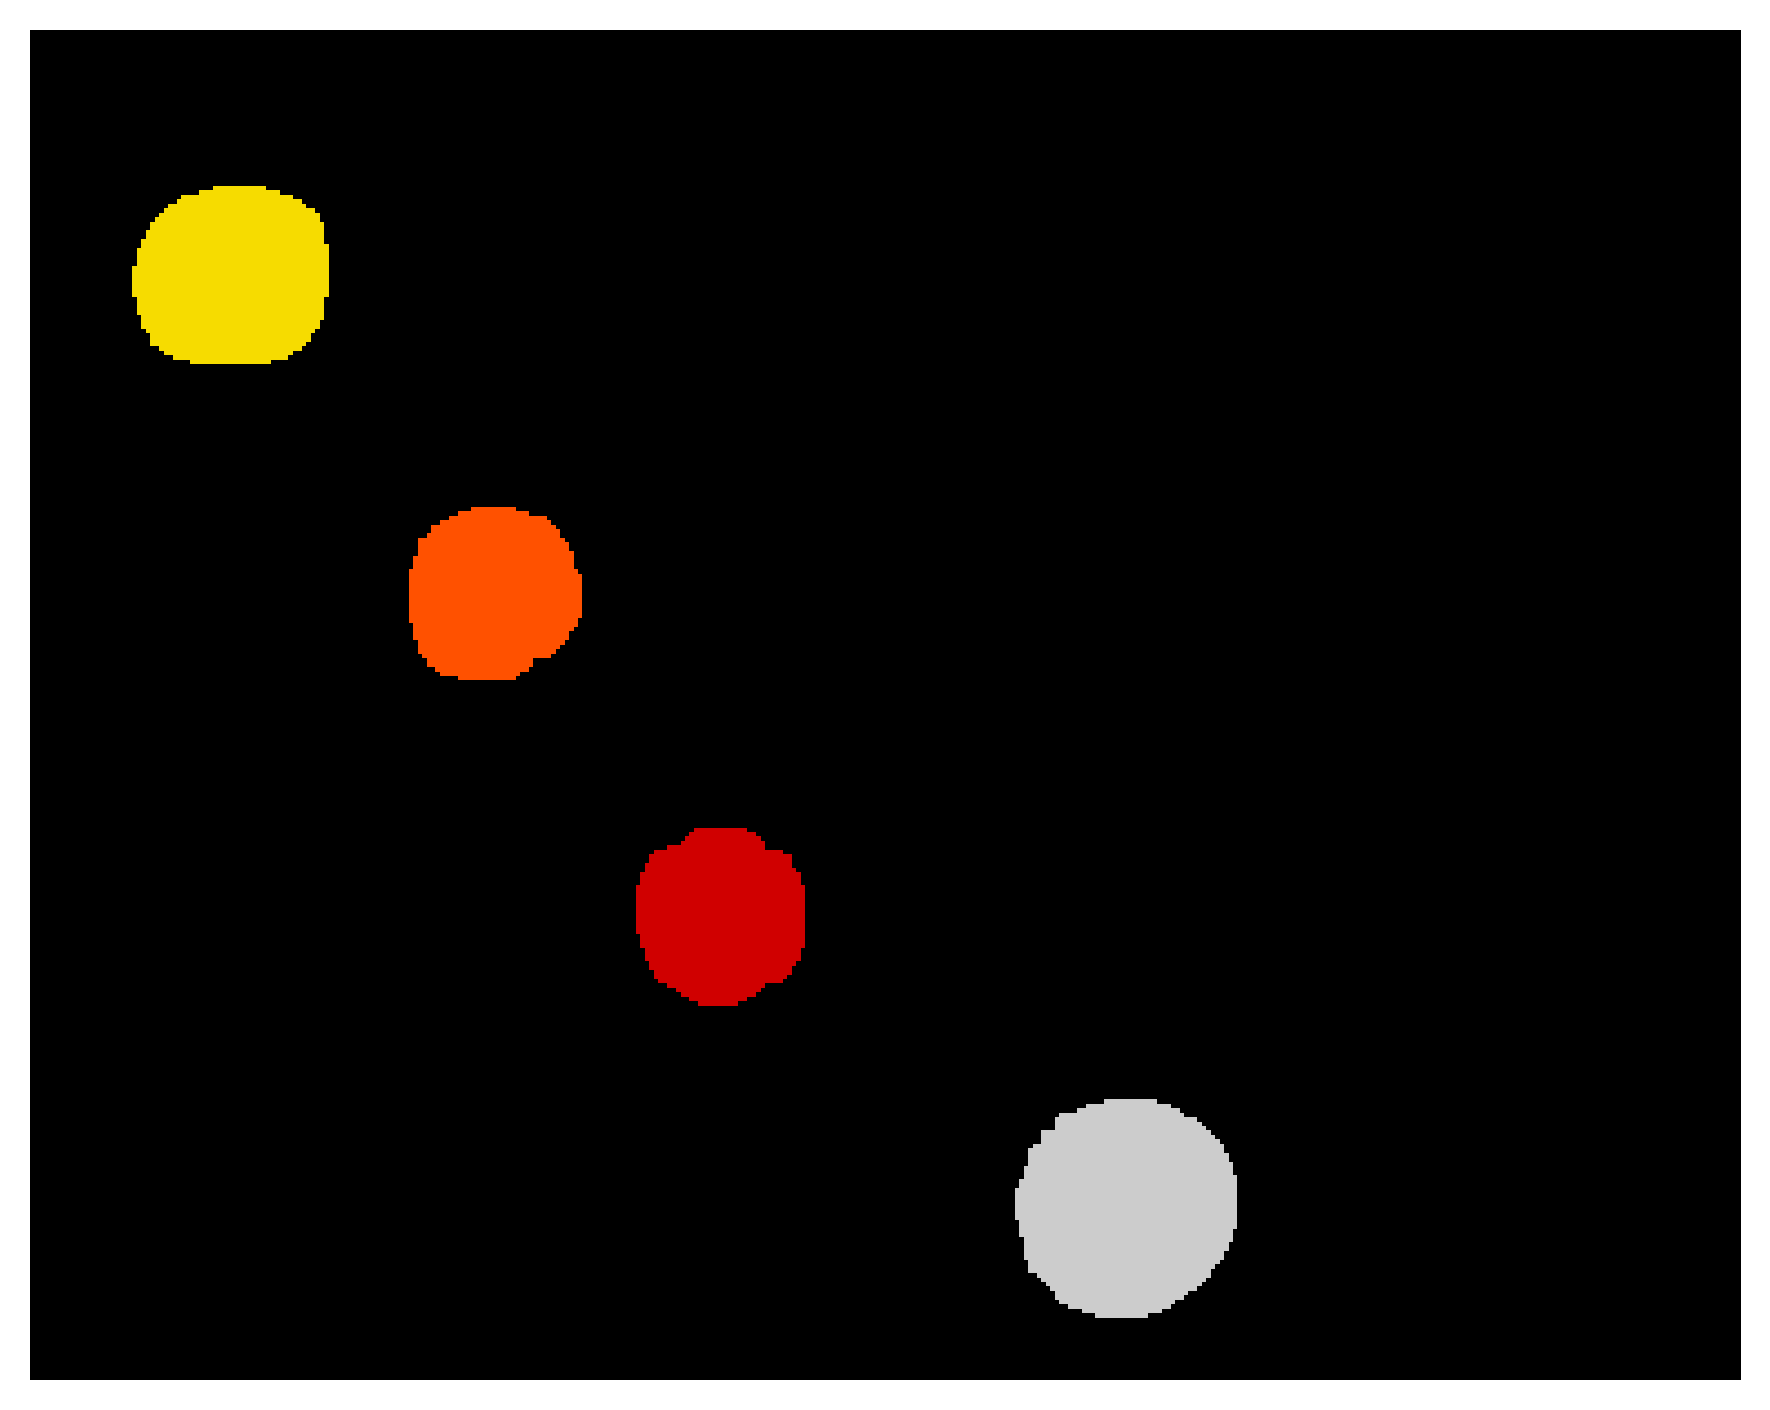
\includegraphics[width=\linewidth]{figs/q1c_selected_coins.png}
        \caption{}
    \end{subfigure}%
    
    \caption{Detailed steps of the coin segmentation process including: (a) Initial median filtering to remove line artefacts, (b) Canny edge detection to outline the coins, (c) Dilated edges to enhance edge continuity, (d) Identification of connected components to identify background, (e) Mask after background removal, (f) Mask integrated with edges to refine the coin outlines, (g) Binary hole filling to complete the interior of the coins, (h) Median filtered mask to remove spurious edges, (i) Final segmentation after eliminating small connected components to isolate individual coins, (j) Identified coins with their grid positions, (k) Selected coins based on specified positions.}
    \label{fig:coin_segmentation_steps}
\end{figure}

\subsubsection{Results}
The final segmentation of the coin image is shown in Figure \ref{fig:q1c_selected_coins}. The segmentation clearly captures the required coins in the specified grid positions.  

\begin{figure}[H]
    \centering
    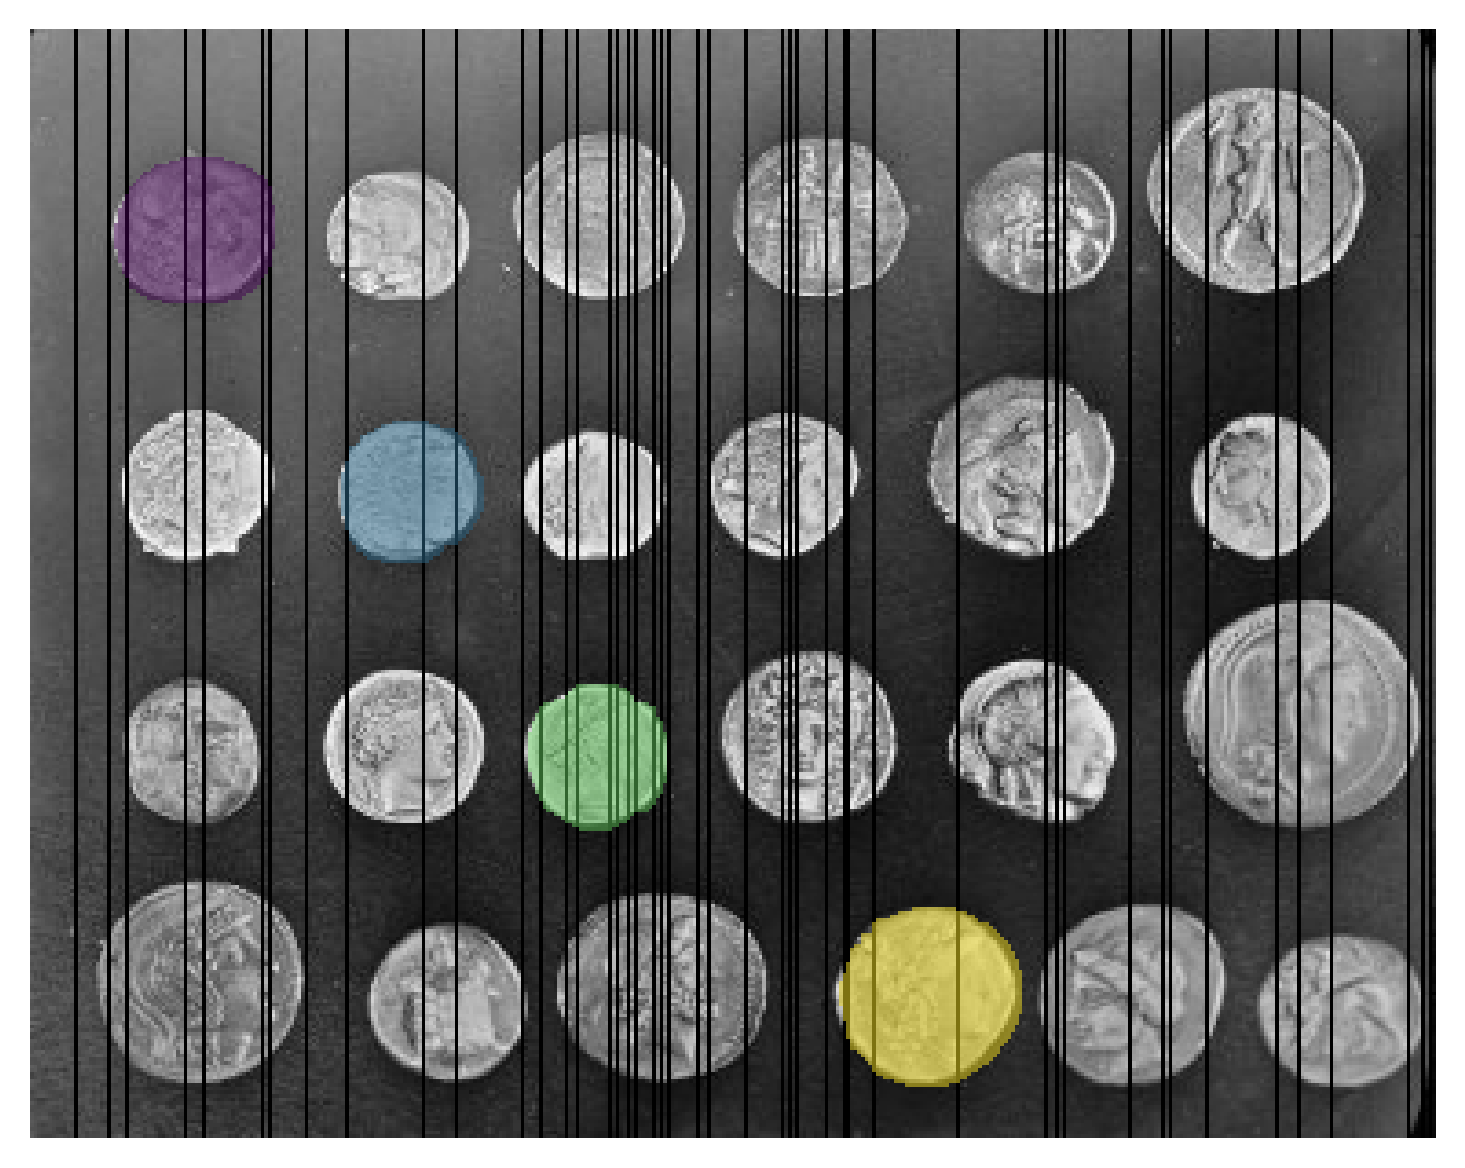
\includegraphics[width=0.8\textwidth]{figs/q1c.png}
    \caption{Final segmentation of the coin image.}
    \label{fig:q1c_selected_coins}
\end{figure}

\subsubsection{Discussion}
The chosen method works almost perfectly, the only issue is that the median filtering and edge dilation steps can result in the final mask being slightly unfaithful to the actual coin shapes around the edge. However, with more experimentation the current approach could be improved to better capture the coin shapes.

\section{Question 2 - Inverse Problems and Multi-resolution analysis}
\subsection{Part A - Solving Over Determined Inverse Problems: Line Fitting}
In this scenario, the goal is to fit a line described by the equation \( y = ax + c \) to a dataset consisting of noisy measurements. This is a typical example of a linear inverse problem where we aim to determine the parameters of a line, which in mathematical terms can be framed as:
\[
y = Ax + b.
\]
Here:
\begin{itemize}
    \item \(y\) is the vector of observed \(y\)-coordinates from the dataset, representing the outputs or dependent variables.
    \item \(A\) is the system matrix that incorporates the independent variable data. For each measurement pair \((x_i, y_i)\), the matrix \(A\) contains a row \([x_i, 1]\) to account for the slope and the intercept of the line.
    \item \(x\) is the vector of parameters to be estimated, specifically \([a, c]\), where \(a\) is the slope and \(c\) is the intercept of the line.
    \item \(b\) represents the vector of measurement errors.
\end{itemize}
This linear regression problem is tackled for two datasets describing noisy line measurements. Both datasets are depicted in Figure \ref{fig:line_fitting_data}, illustrating the points used for line fitting. It is worth noting that the second dataset is identical to the first for all points except for one which is modified to describe an outlier point. 

This system is over-determined for the given datasets because there are more measurements (\(20\) pairs of \(x, y\) values) than there are parameters to estimate (just two, \(a\) and \(c\)). Although over-determined systems may be well posed and have a unique solution and when all measurements are consistent with the true signal. However, in the presence of noise, the system will not have any exact solutions, where all data points lie perfectly on the same line. Instead, the objective is to find the best estimates for the parameters \(x = [a, c]\) that minimise the difference between the predicted line \( Ax \) and the observed data \( y \), via the objective function. In this problem, the \(L_2\) and \(L_1\) norms of the error vector, $\epsilon = y - Ax$, are explored as the objective functions. 


\begin{figure}[H]
    \centering
    \begin{subfigure}{.45\textwidth}
        \centering
        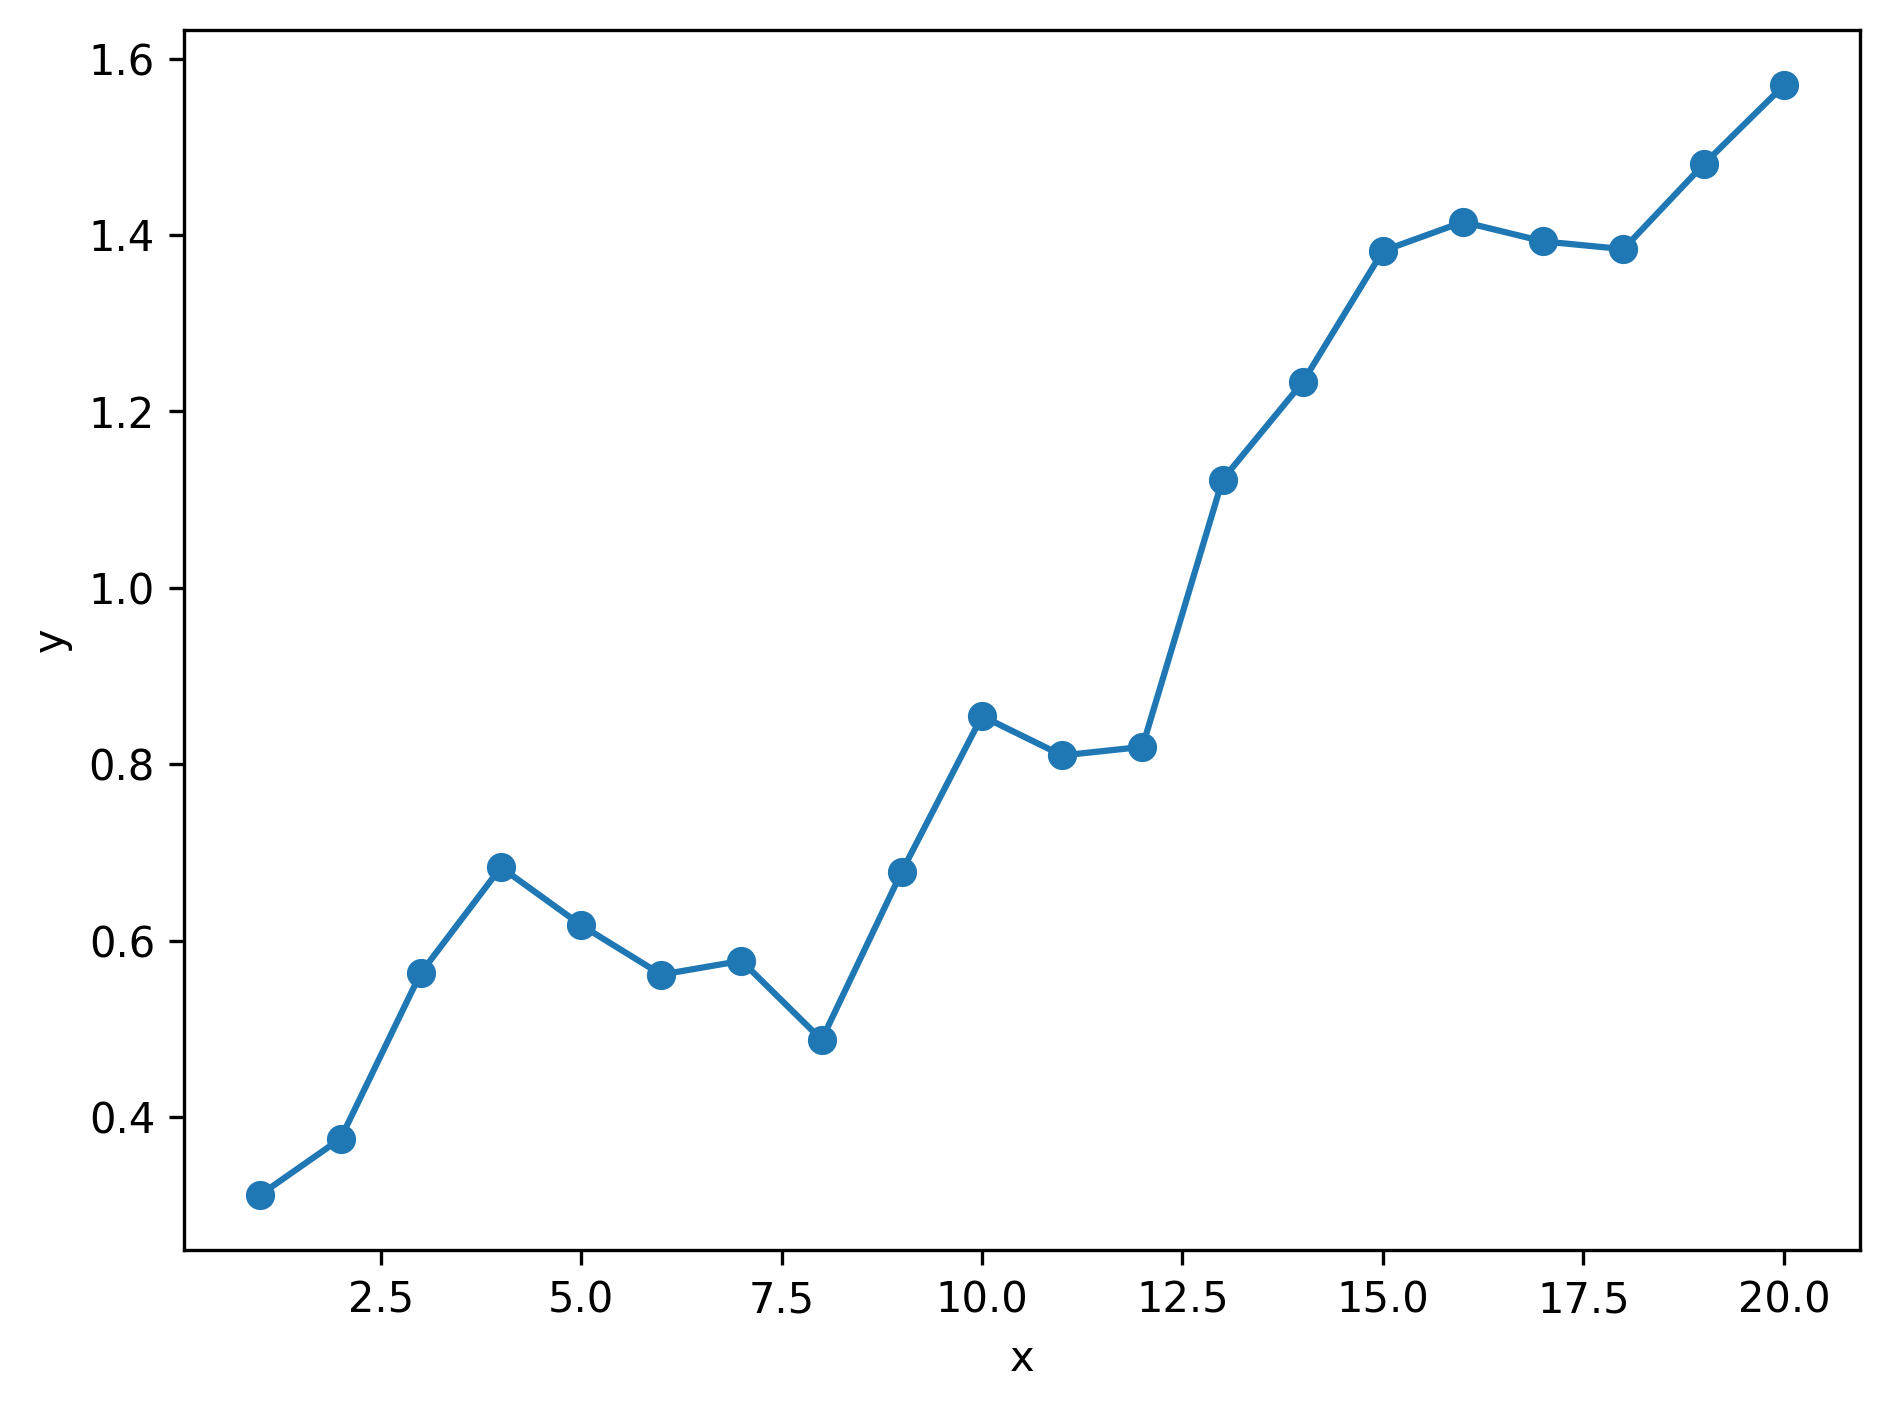
\includegraphics[width=\linewidth]{figs/q2a_noisy_line.png}
        \caption{}
        \label{fig:line_data_1}
    \end{subfigure}%
    \begin{subfigure}{.45\textwidth}
        \centering
        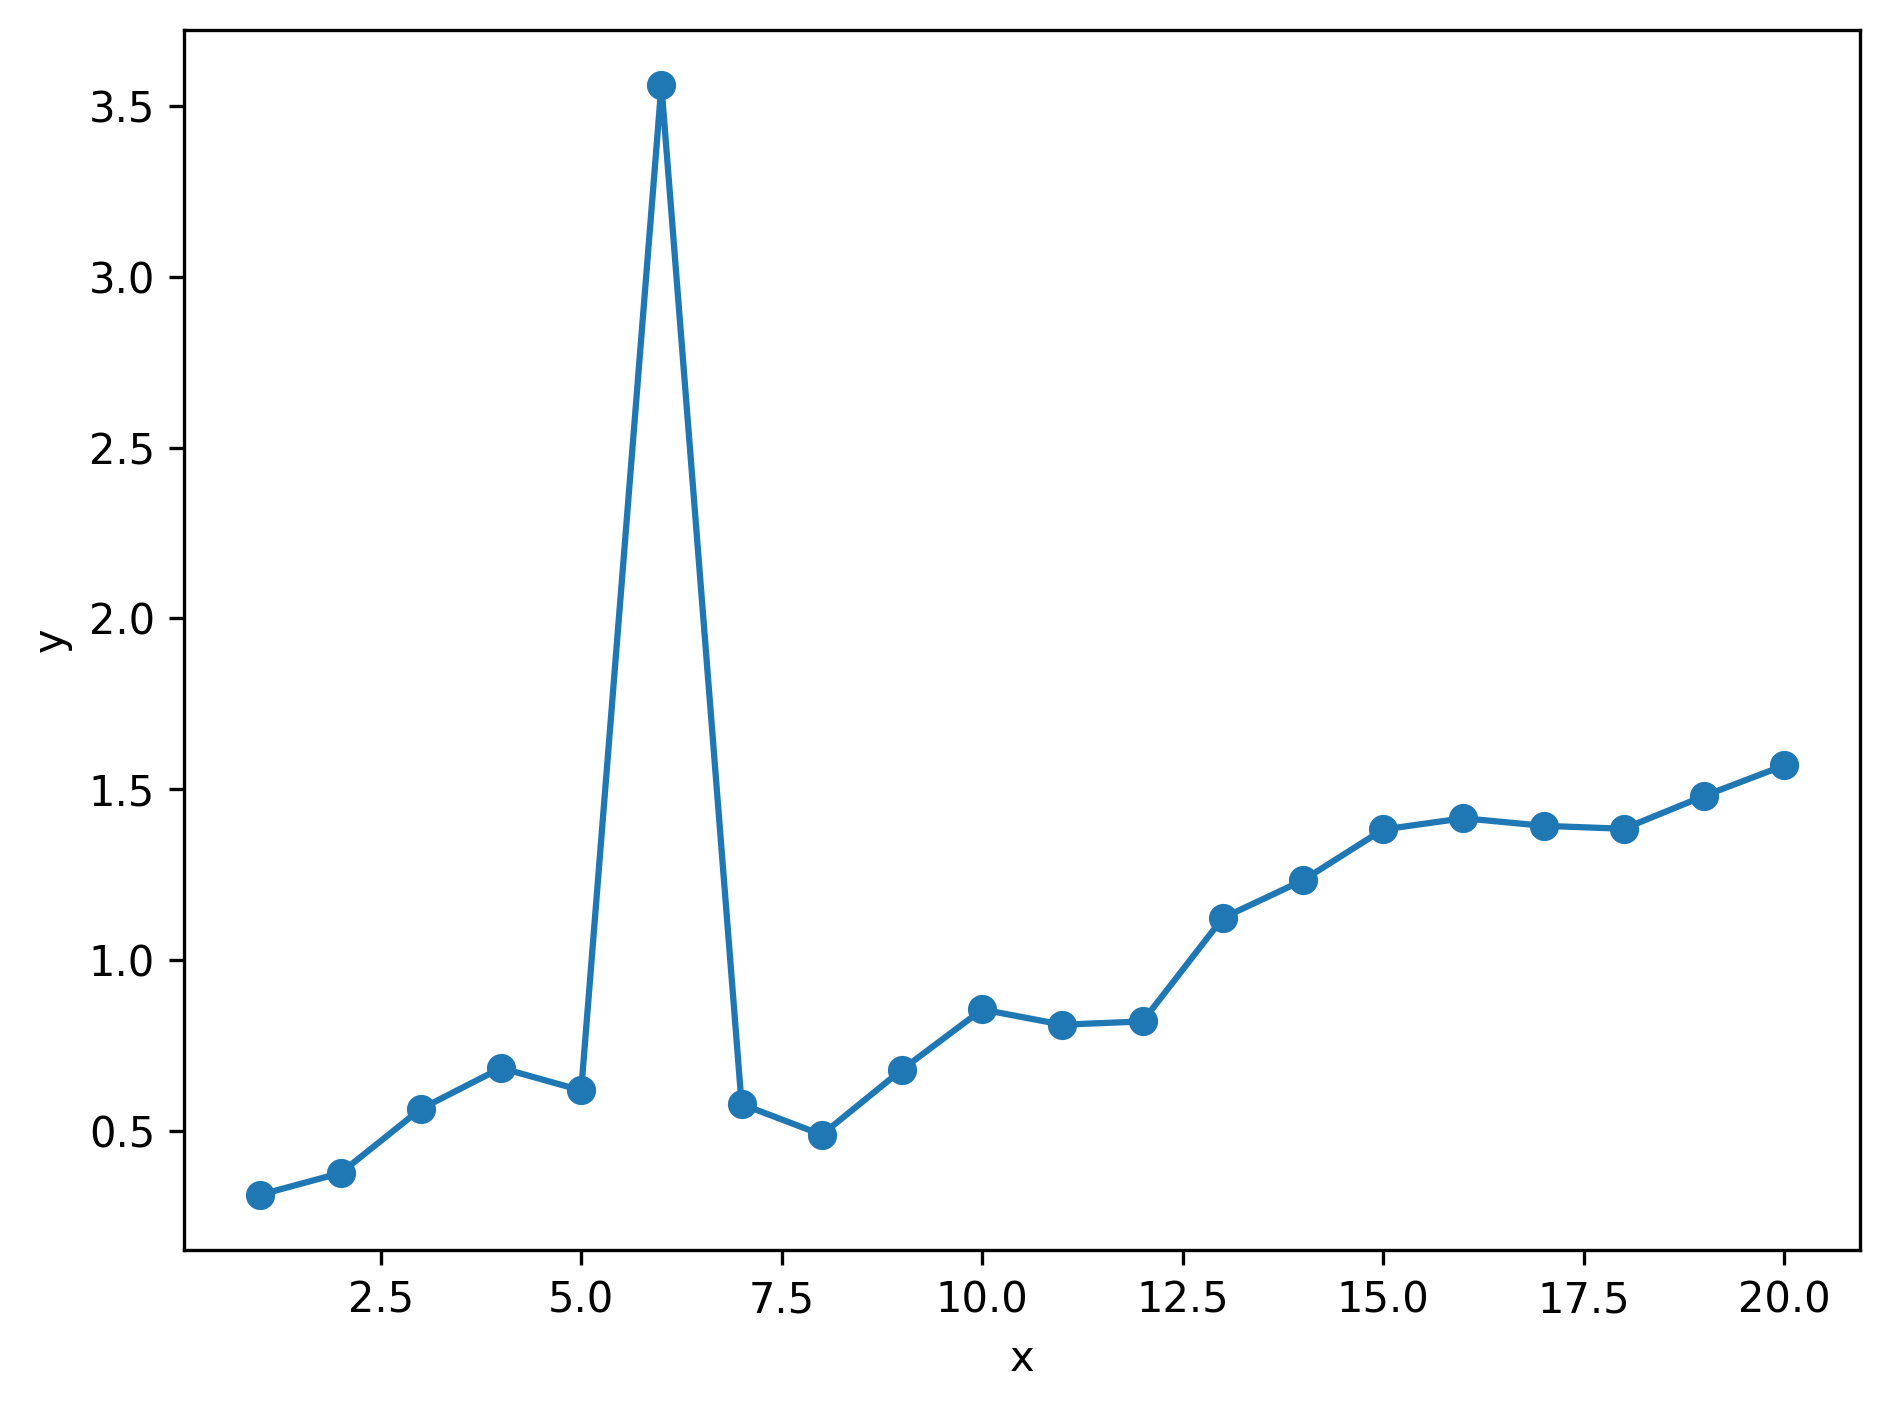
\includegraphics[width=\linewidth]{figs/q2a_noisy_line_outlier.png}
        \caption{}
        \label{fig:line_data_2}
    \end{subfigure}%
    \caption{Two datasets describing noisy measurements of points along a line: (a) Dataset 1 - line data with noisy observations (b) Dataset 2 - line data with noisy observations and a single outlier.}
    \label{fig:line_fitting_data}
\end{figure}
% Describe the method used to solve the problem in 2a
\subsubsection{Results}
To minimise the objective function for the given datasets, the \texttt{minimize} function from the \texttt{scipy.optimize} library is employed. This function uses the SLSQP optimisation algorithm to find the minimum of the objective function \cite{Kraft1988}. The results of the line fitting for the two datasets are shown in Figure \ref{fig:line_fitting_results} and the estimated line parameters are summarised in Table \ref{tab:line_fitting_results}.

\begin{figure}[H]
    \centering
    \begin{subfigure}{.45\textwidth}
        \centering
        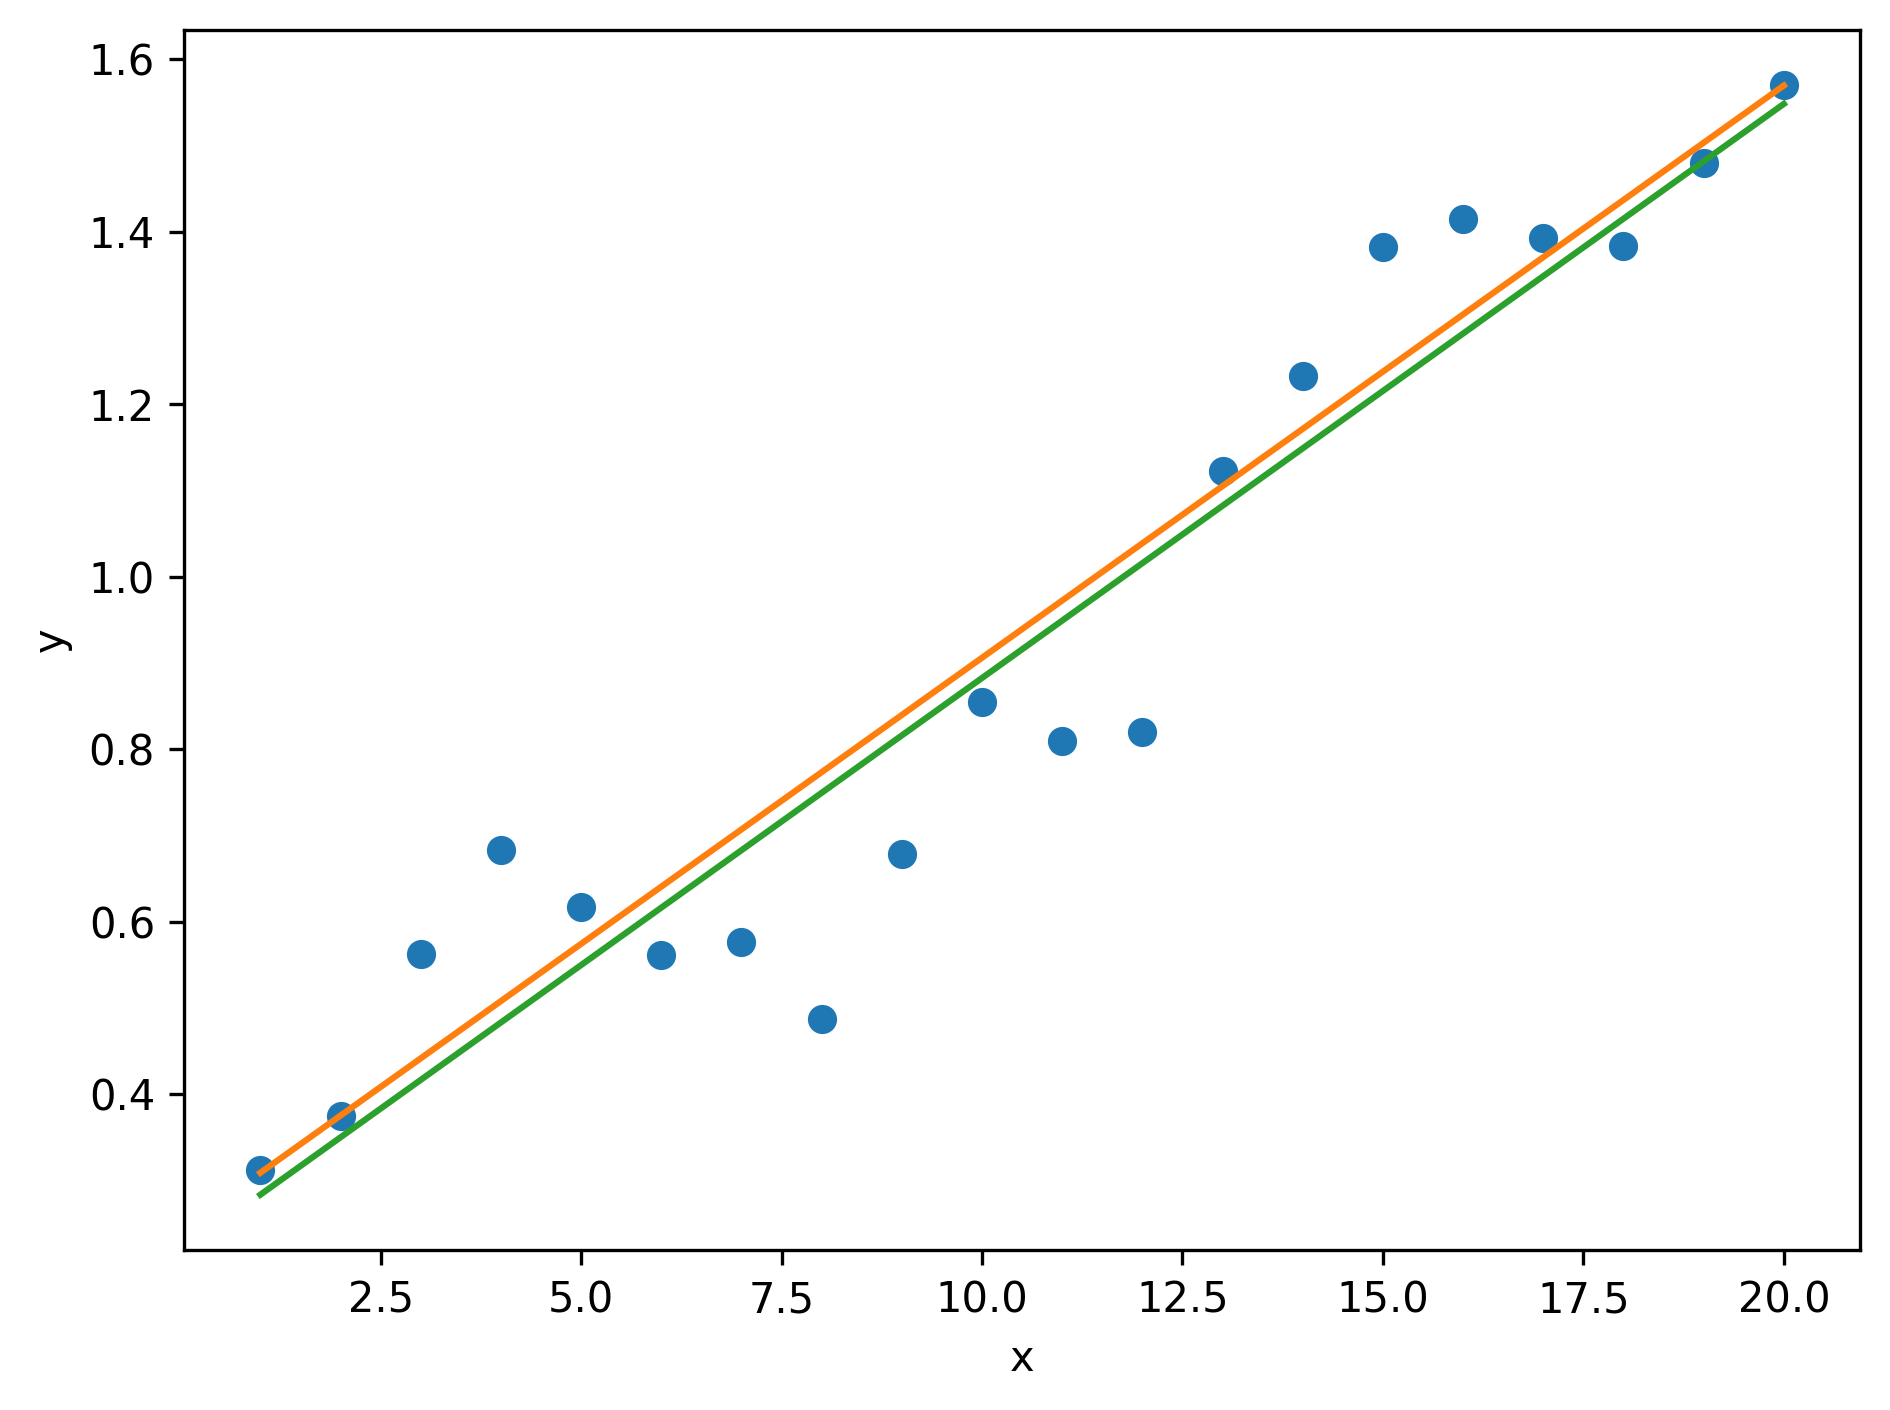
\includegraphics[width=\linewidth]{figs/q2a_fitted_line_1.png}
        \caption{}
        \label{fig:line_fit_1}
    \end{subfigure}%
    \begin{subfigure}{.45\textwidth}
        \centering
        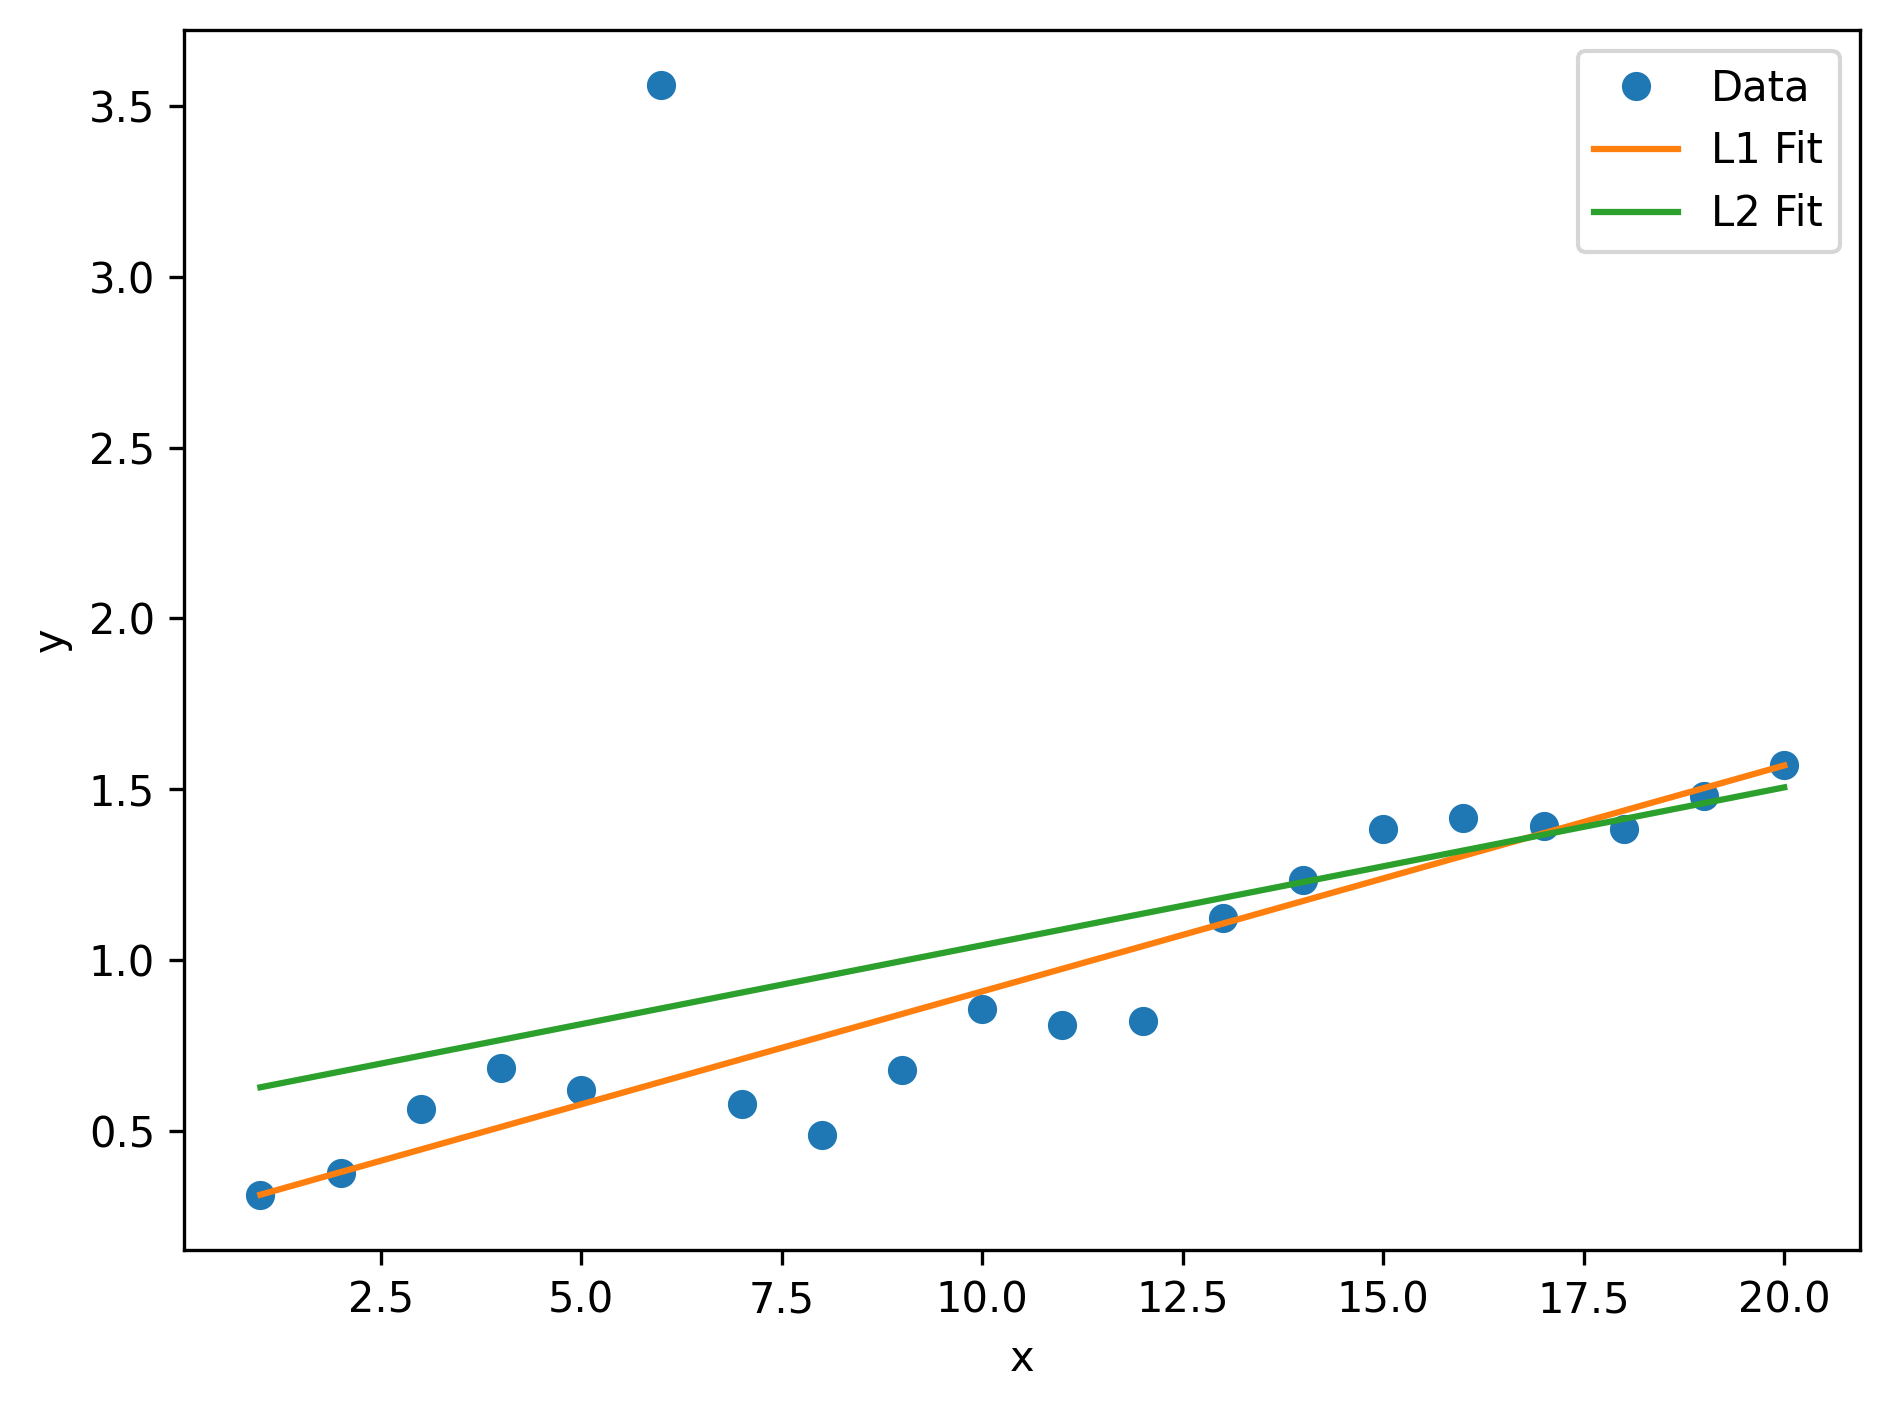
\includegraphics[width=\linewidth]{figs/q2a_fitted_line_2.png}
        \caption{}
        \label{fig:line_fit_2}
    \end{subfigure}%
    \caption{Results of line fitting using the SLSQP optimization algorithm to minimise the \(L_2\) and \(L_1\) error norms for the two datasets, which are shown in green and orange respectively: (a) Dataset 1, (b) Dataset 2 with the outlier.}
    \label{fig:line_fitting_results}
\end{figure}

\begin{table}[H]
    \centering
    \begin{tabular}{@{}llll@{}}
    \toprule
    \textbf{Dataset} & \textbf{Objective Function} & \textbf{Slope (a)} & \textbf{Intercept (c)} \\ \midrule
    1               & \(L_2\) Norm                & 0.0665             & 0.2172                 \\
                    & \(L_1\) Norm                & 0.0663             & 0.2429                 \\ \midrule
    2               & \(L_2\) Norm                & 0.0462             & 0.5804                 \\
                    & \(L_1\) Norm                & 0.0662             & 0.2458                 \\ \bottomrule
    \end{tabular}
    \caption{Summary of the estimated line parameters for the two datasets using the \(L_2\) and \(L_1\) error norms.}
    \label{tab:line_fitting_results}
\end{table}

\subsubsection{Discussion}
In the absence of outliers, both \(L_2\) and \(L_1\) norms provide comparable results for line fitting. However, when outliers are present, the \(L_1\) norm offers a more accurate estimation because it minimises the absolute errors, which reduces the impact of extreme values. Conversely, the \(L_2\) norm, which minimises the sum of squared errors, gives disproportionately high weight to outliers. This sensitivity causes the \(L_2\) norm to be more influenced by the outlier, skewing the line fit significantly away from the majority of the data points, as observed in the results for the second dataset.



\subsection{Part B - Compressed Sensing Reconstruction and Underdetermined Inverse Problems}
% Introduce the problem 
This question explores signal reconstruction within the compressed sensing framework, which leverages a powerful observation: many signals of interest are sparse when represented in an appropriate basis. Mathematically, a signal \( x \in \mathbb{R}^n \) is considered \( K \) sparse if it can be expressed as \( x = \Psi s \) where \( \Psi \) is some universal basis matrix and \( s \) has only \( K \) non-zero elements, with \( K \ll n \). Compressed sensing capitalizes on this sparsity to reconstruct signals from measurements taken below the traditional Nyquist rate, which dictates the minimum number of uniform samples needed to avoid aliasing. In the compressed sensing paradigm, measurements \( y \) are obtained by sub sampling with a non-uniform or random measurement matrix \( C \). The goal is to recover the original signal \( x \) by solving the underdetermined system of equations for \( s \) and applying the transformation \( \Psi \) to reconstruct the signal. To solve the underdetermined system, a solution is sought that minimises the \( L_1 \) norm of the coefficient vector \( s \) under the constraint that the measurements \( y \) are consistent with the signal model. The \( L_1 \) norm is used as a regularisation term to promote sparsity in the solution, leveraging the prior knowledge that the signal is sparse in the transformed domain. Mathematically, this problem can be represented as the following optimisation problem:
\[
\argmin_{s} \left\| s \right\|_1 \quad \text{subject to} \quad y = C \Psi s.
\]

This problem can be solved iteratively using a combination of soft thresolding in the sparse domain and enforcing consistency in the measurement domain \cite{doi:10.1137/080716542}. 

\paragraph*{Conditions for Compressed Sensing}
Beyond the requirement of signal sparsity in the transformed domain, successful application of compressed sensing requires the following conditions to be satisfied:
\begin{enumerate}
    \item \textbf{Incoherence of Measurement Matrix:}
    The measurement matrix \( C \) must be incoherent with respect to the sparsifying basis \( \Psi \). Incoherence here implies that the rows of \( C \) are not correlated with the columns of \( \Psi \). High incoherence between \( C \) and \( \Psi \) ensures that the measurements \( y \) contain sufficient information about all the components of the sparse signal \( s \), thereby facilitating accurate recovery even from fewer observations.
    
    \item \textbf{Sufficient Number of Measurements:}
    The minimum number of measurements \( p \) must be of the order of:
    \[
    p \approx O(K \log(N/K))),
    \]
    where \( K \) is the sparsity level (number of non-zero entries in \( s \)), \( N \) is the dimension of the signal \( x \).
\end{enumerate}

\subsubsection{Problem Set Up}
To practically demonstrate compressed sensing reconstruction, a 1D sparse signal \( s \) of size 100 is generated with only 10 non-zero coefficients. To simulate real world conditions, zero mean gaussian noise is added with standard deviation 0.05 to the signal. This is the sparse signal in the time domain. The signal is then transformed into the fourier domain using the discrete fast fourier transform (DFFT) to obtain the non sparse spectra \( x \). The sparse signal and its fourier transform are shown in Figure \ref{fig:compressed_sensing_signal}. Therefore, \( x = \Psi s \) where \( \Psi \) is the DFFT matrix. 
\begin{figure} [H]
    \centering
    \begin{subfigure}{.45\textwidth}
        \centering
        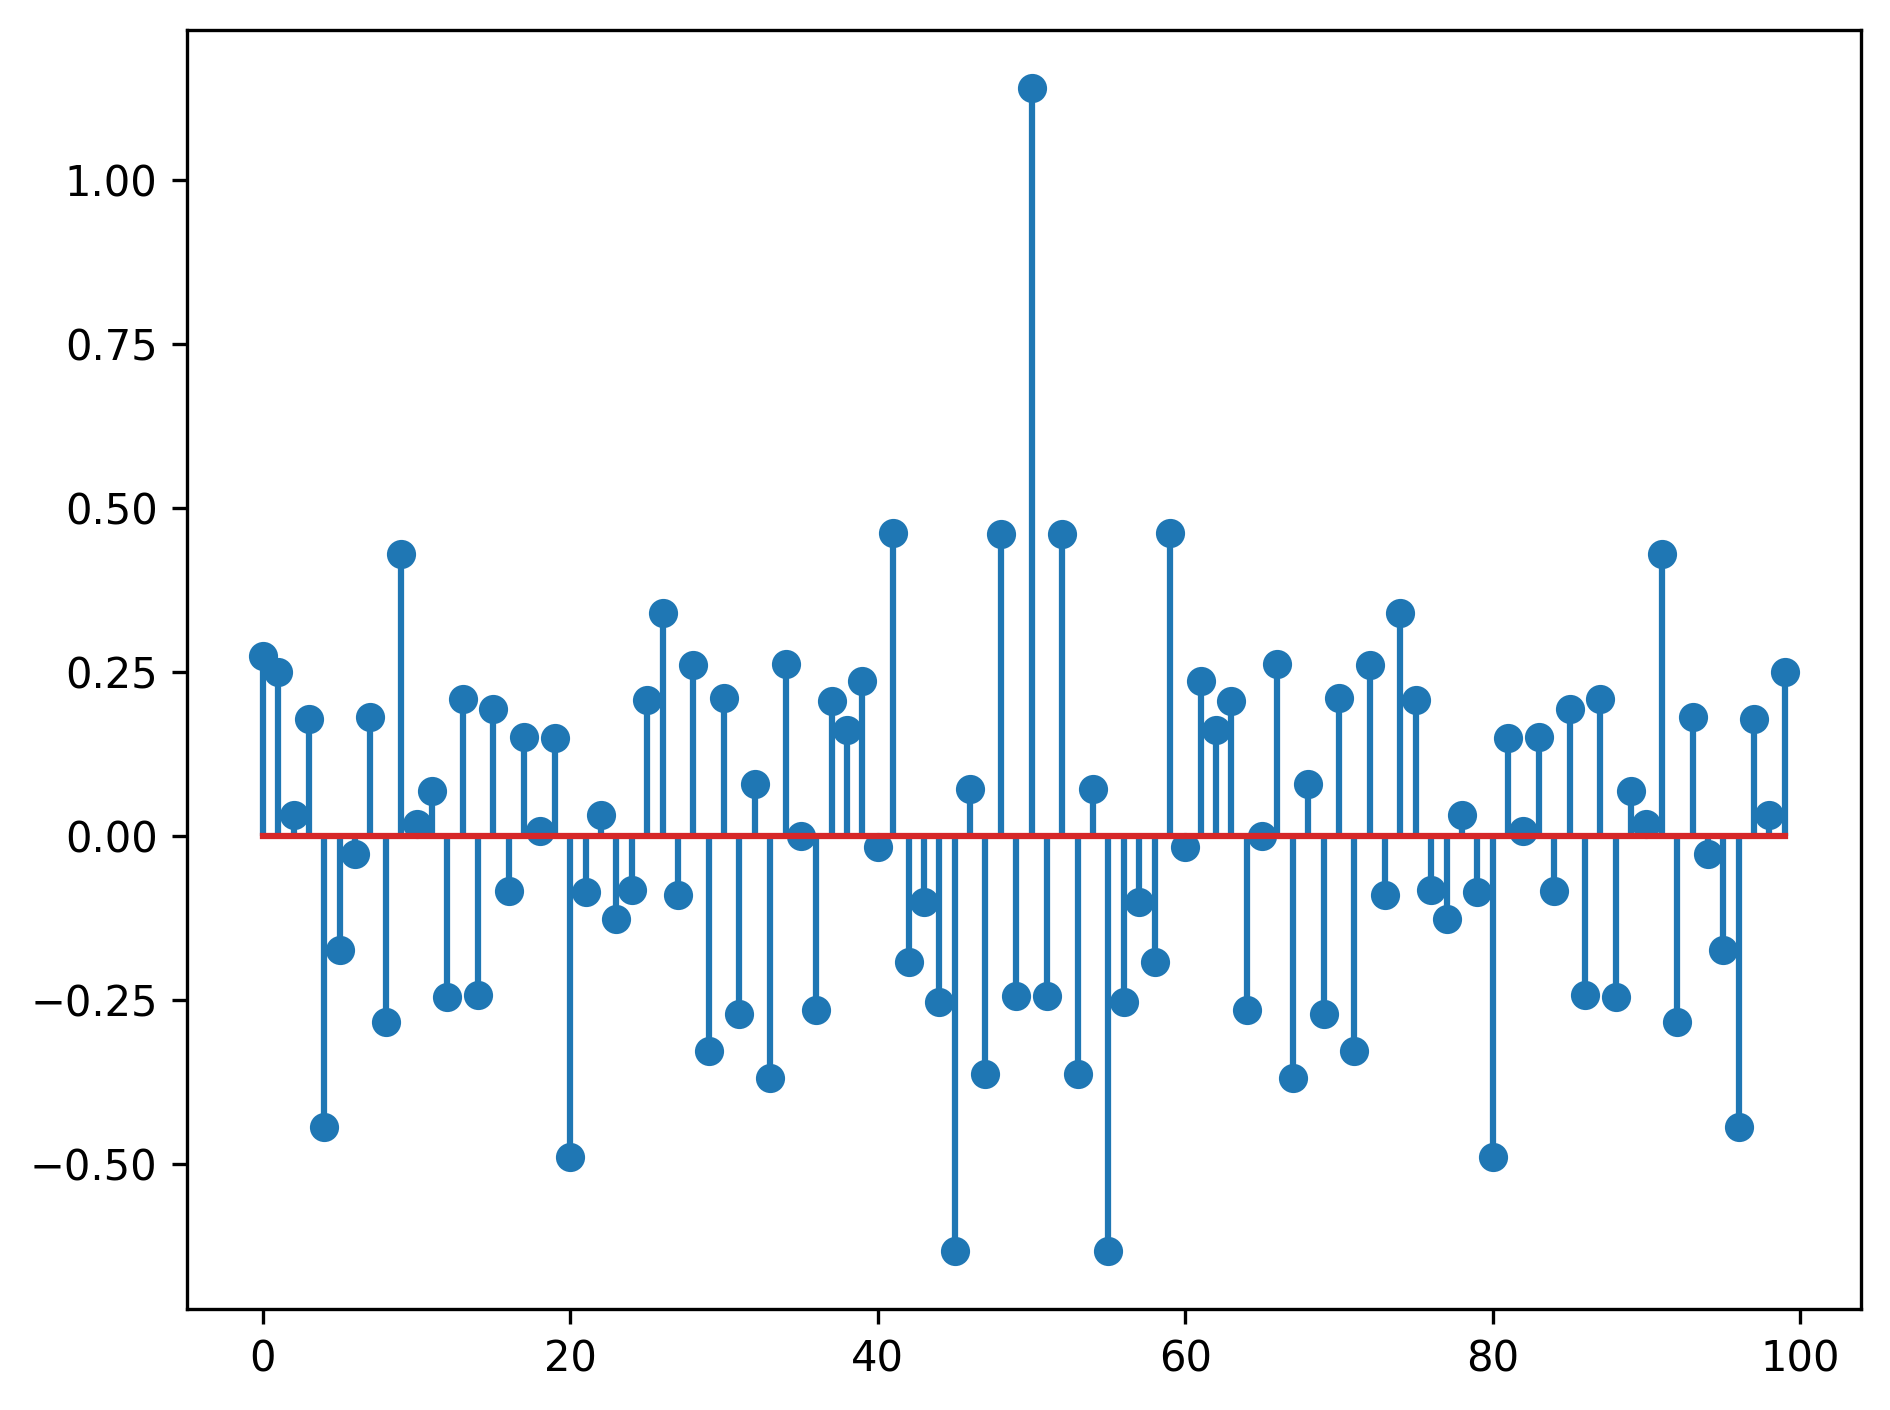
\includegraphics[width=\linewidth]{figs/q2b_original_sparse_signal_fft.png}
        \caption{Frequency domain}
        \label{fig:sparse_signal_fourier}
    \end{subfigure}%
    \begin{subfigure}{.45\textwidth}
        \centering
        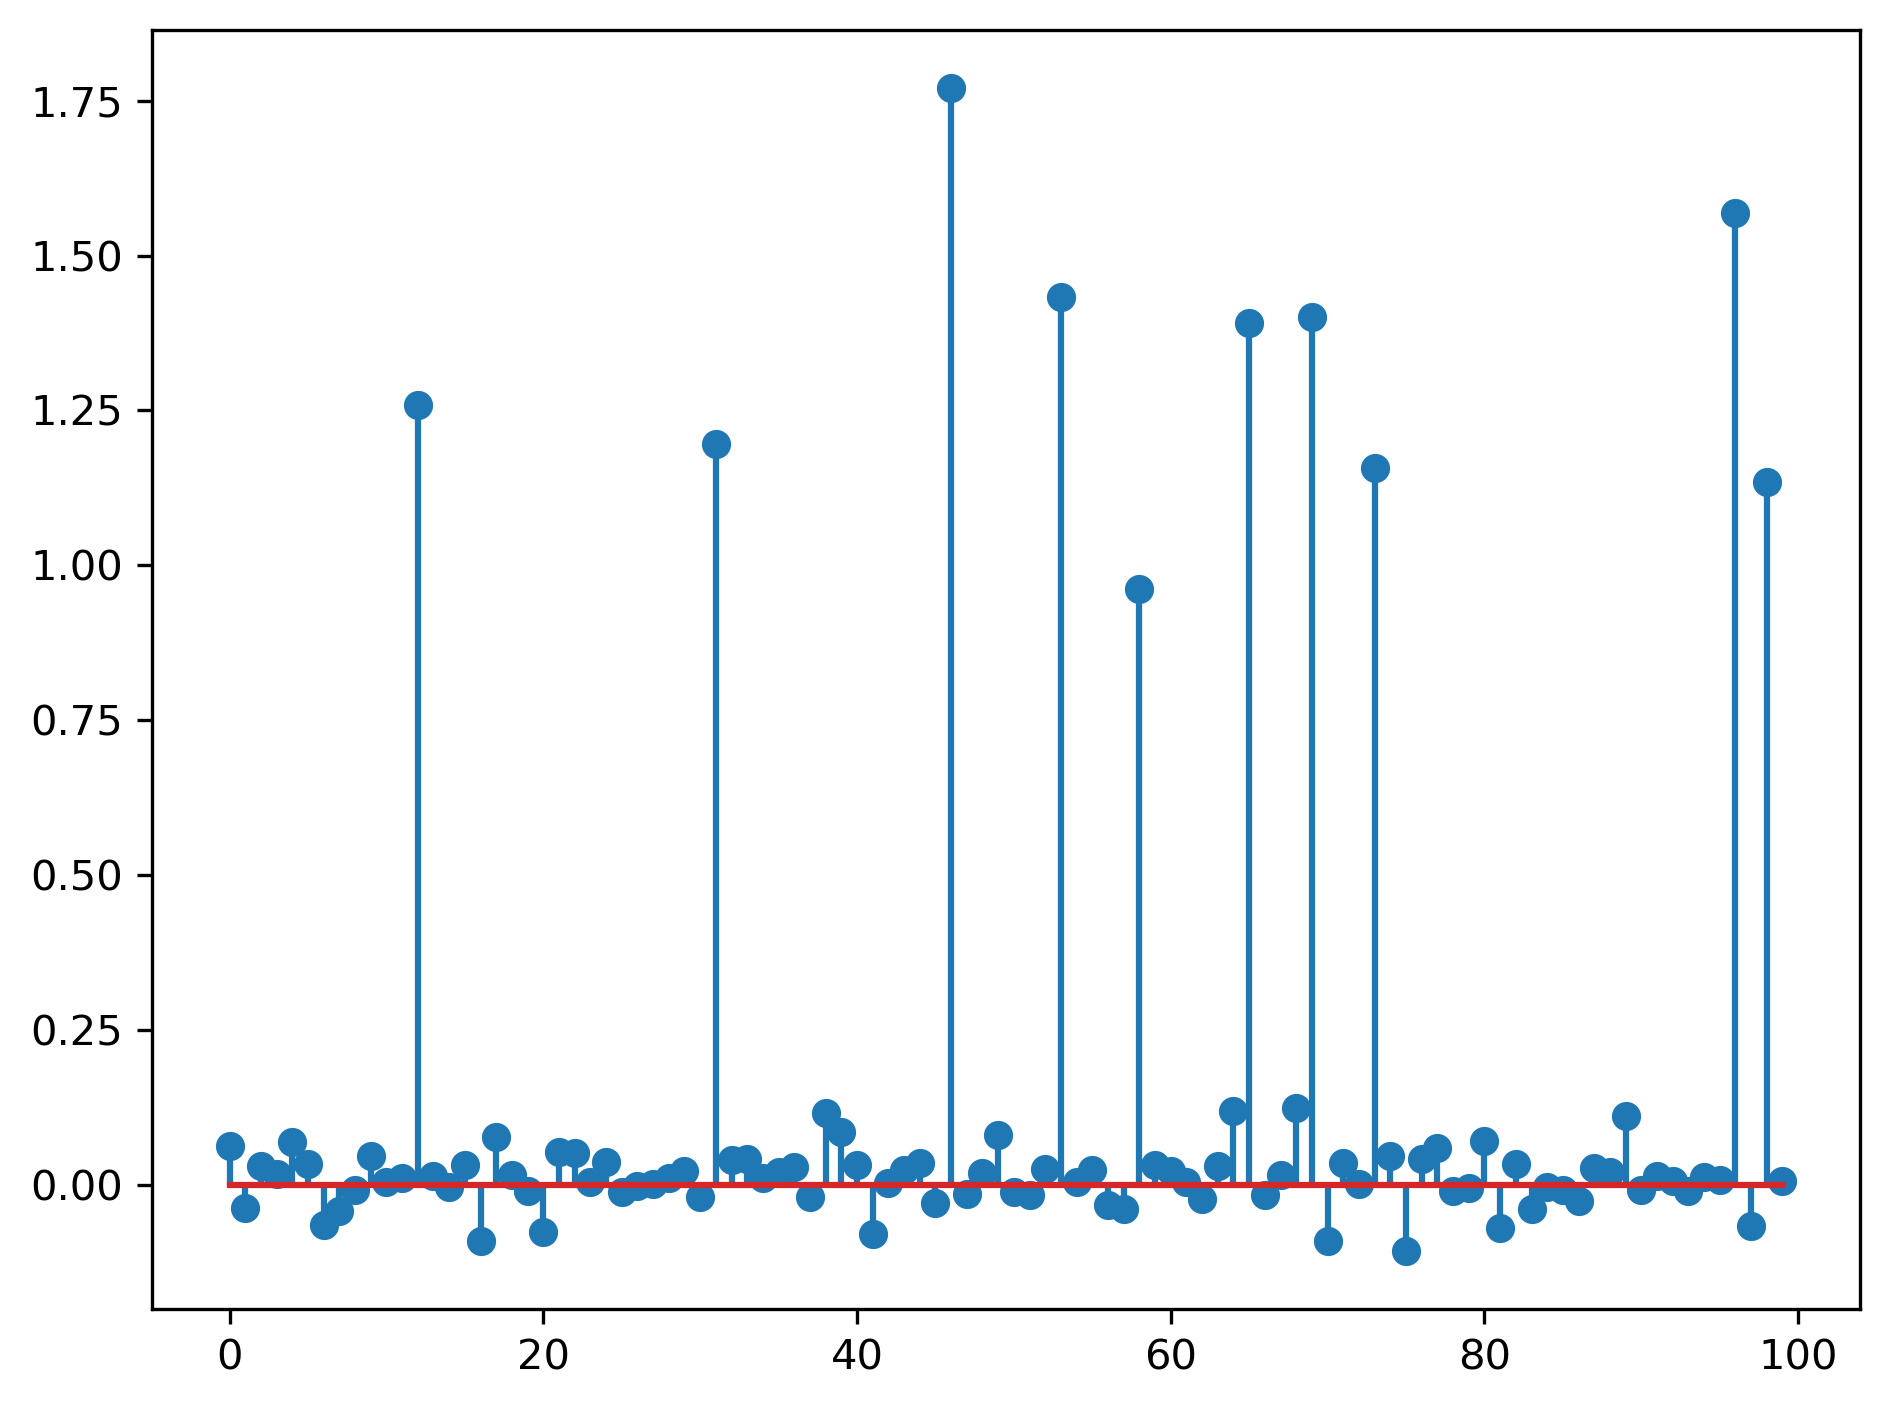
\includegraphics[width=\linewidth]{figs/q2b_original_sparse_signal.png}
        \caption{Time Domain}
        \label{fig:sparse_signal}
    \end{subfigure}%

    \caption{Generated signal expressed in sparse and non sparse domains: (a) Non sparse signal \( x\) in the fourier domain, (b) sparse signal \( s \) in the time domain.}
    \label{fig:compressed_sensing_signal}
\end{figure}

These signals can be seen in Figure \ref{fig:compressed_sensing_signal}. The signal in the non sparse measurement domain, \(x\), is then sub sampled under uniform and random strategies to obtain two sets of 32 measurements \( y \). These sub sampled signals are shown in Figure \ref{fig:compressed_sensing_sub_sampled_signals} in both the time and frequency domains. Note that a correction factor is applied to the IDFFT of \(y\) to account for the sub sampling.

\begin{figure}[H]
    \centering
    % Uniform Sampling Subfigures
    \begin{subfigure}{.45\textwidth}
        \centering
        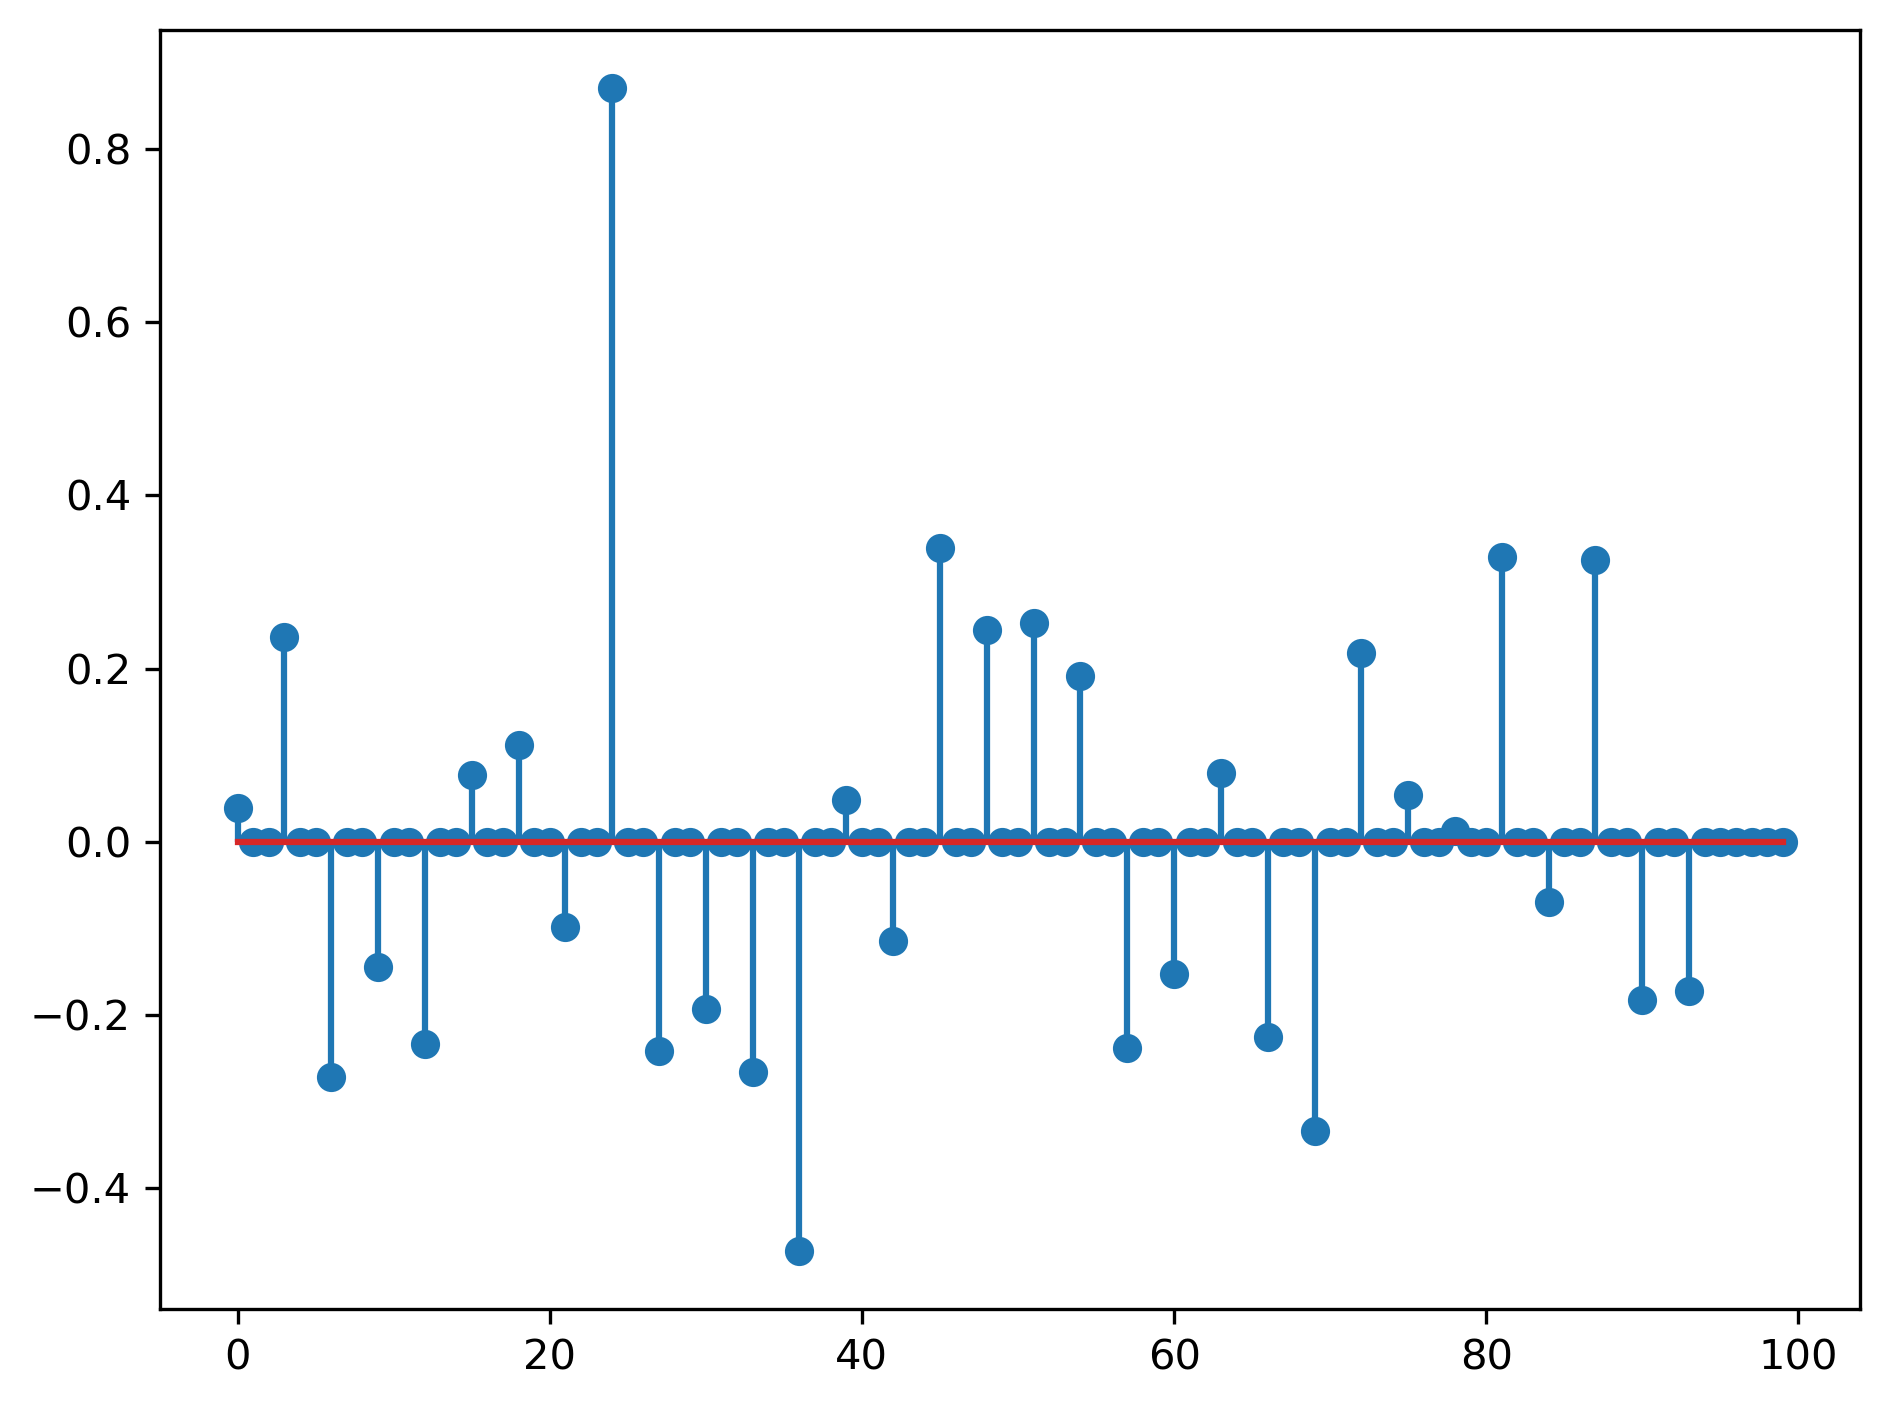
\includegraphics[width=\linewidth]{figs/q2b_uniformly_subsampled_signal_fft.png}
        \caption{Uniform Sampling - Frequency Domain}
        \label{fig:uniform_subsampled_signal_fft}
    \end{subfigure}%
    \begin{subfigure}{.45\textwidth}
        \centering
        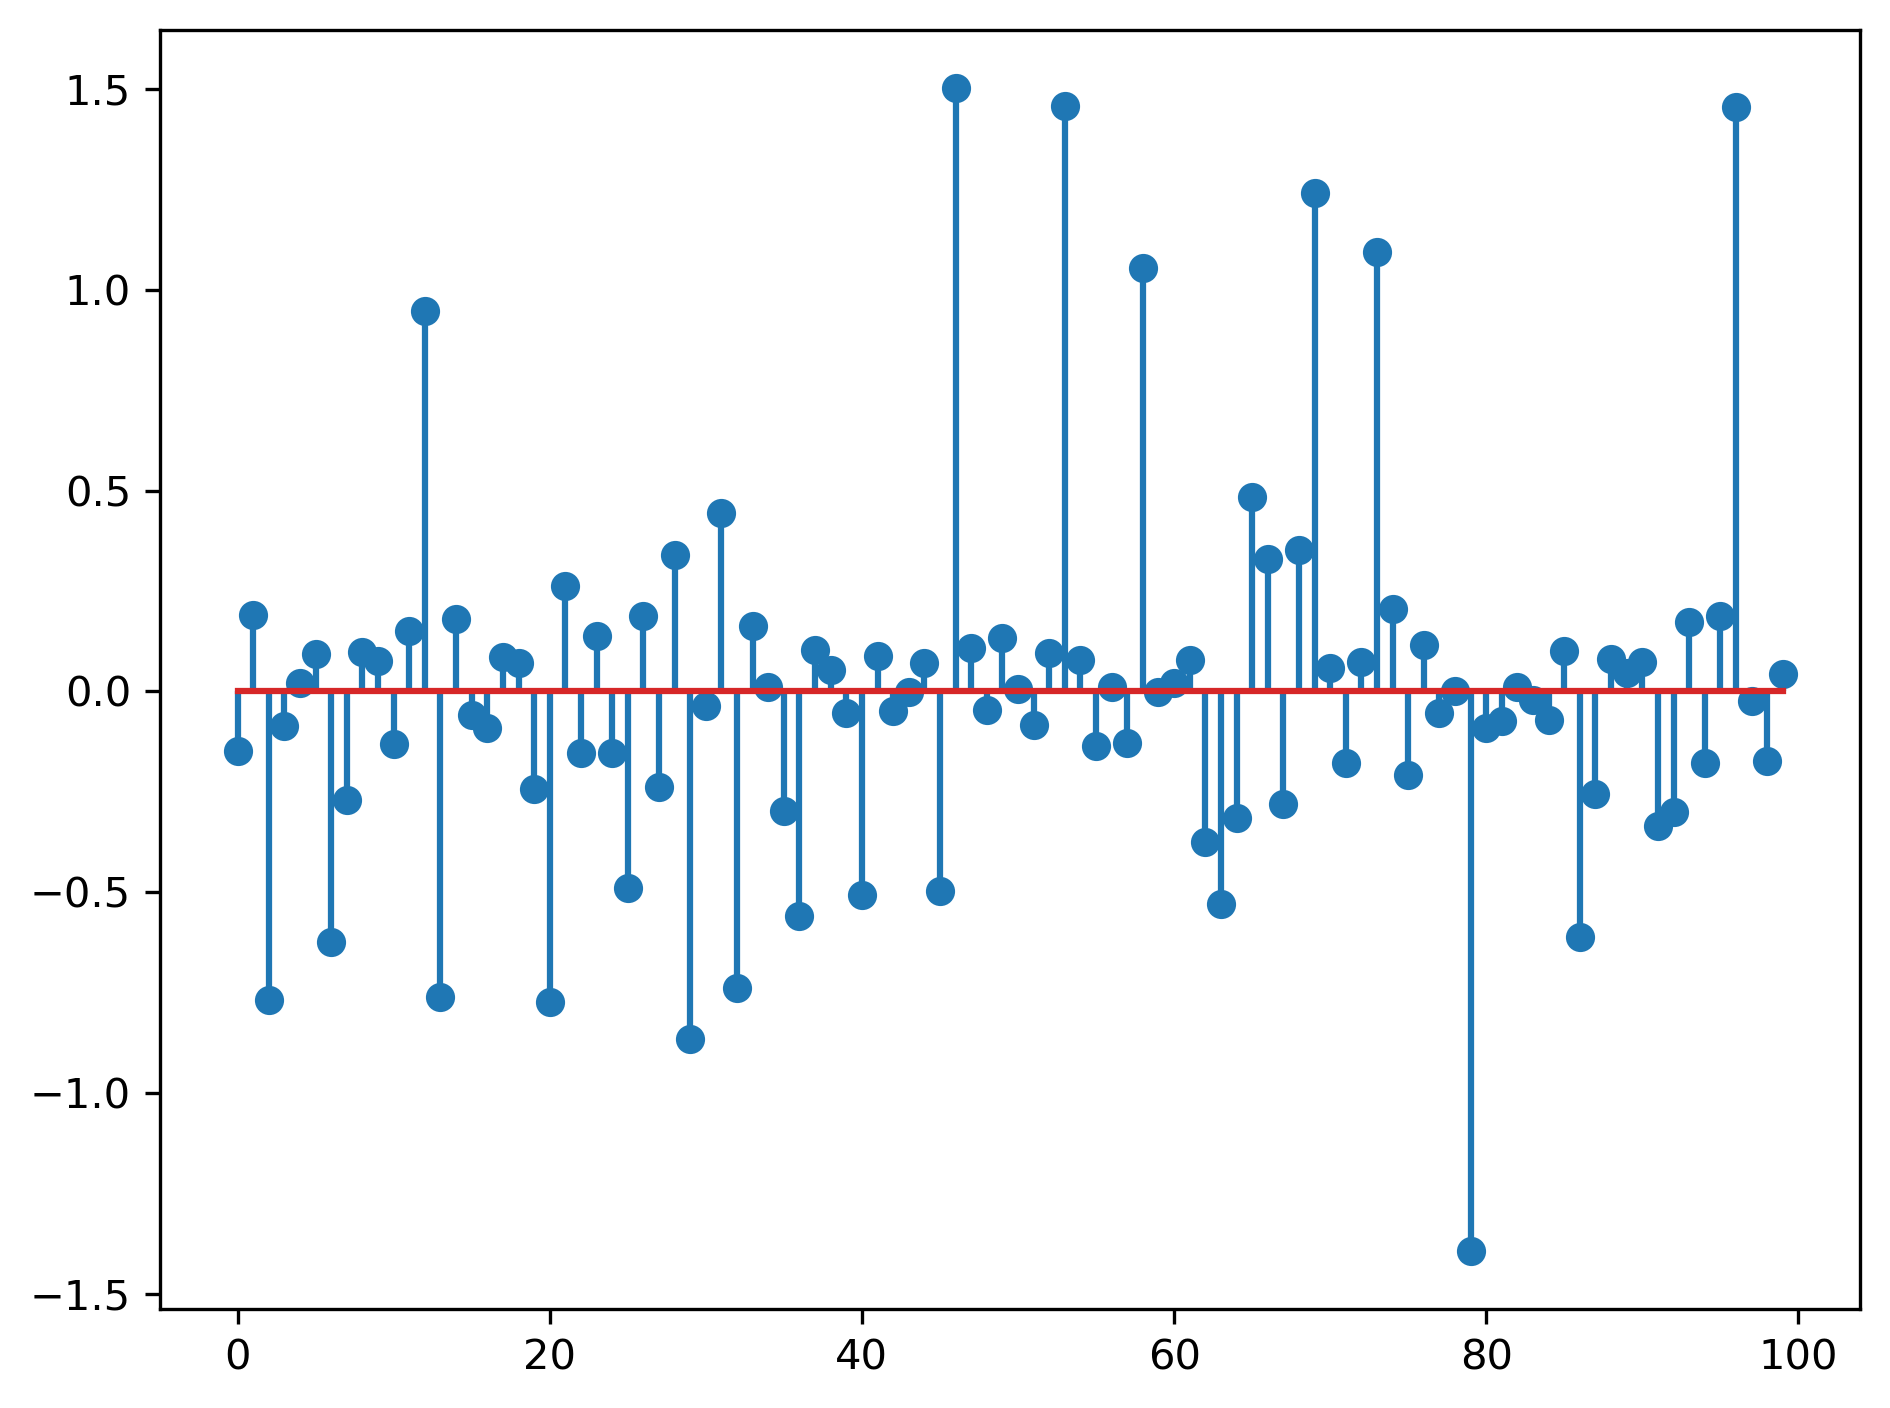
\includegraphics[width=\linewidth]{figs/q2b_uniformly_subsampled_signal.png}
        \caption{Uniform Sampling - Time Domain}
        \label{fig:uniform_subsampled_signal}
    \end{subfigure}
    
    % Random Sampling Subfigures
    \begin{subfigure}{.45\textwidth}
        \centering
        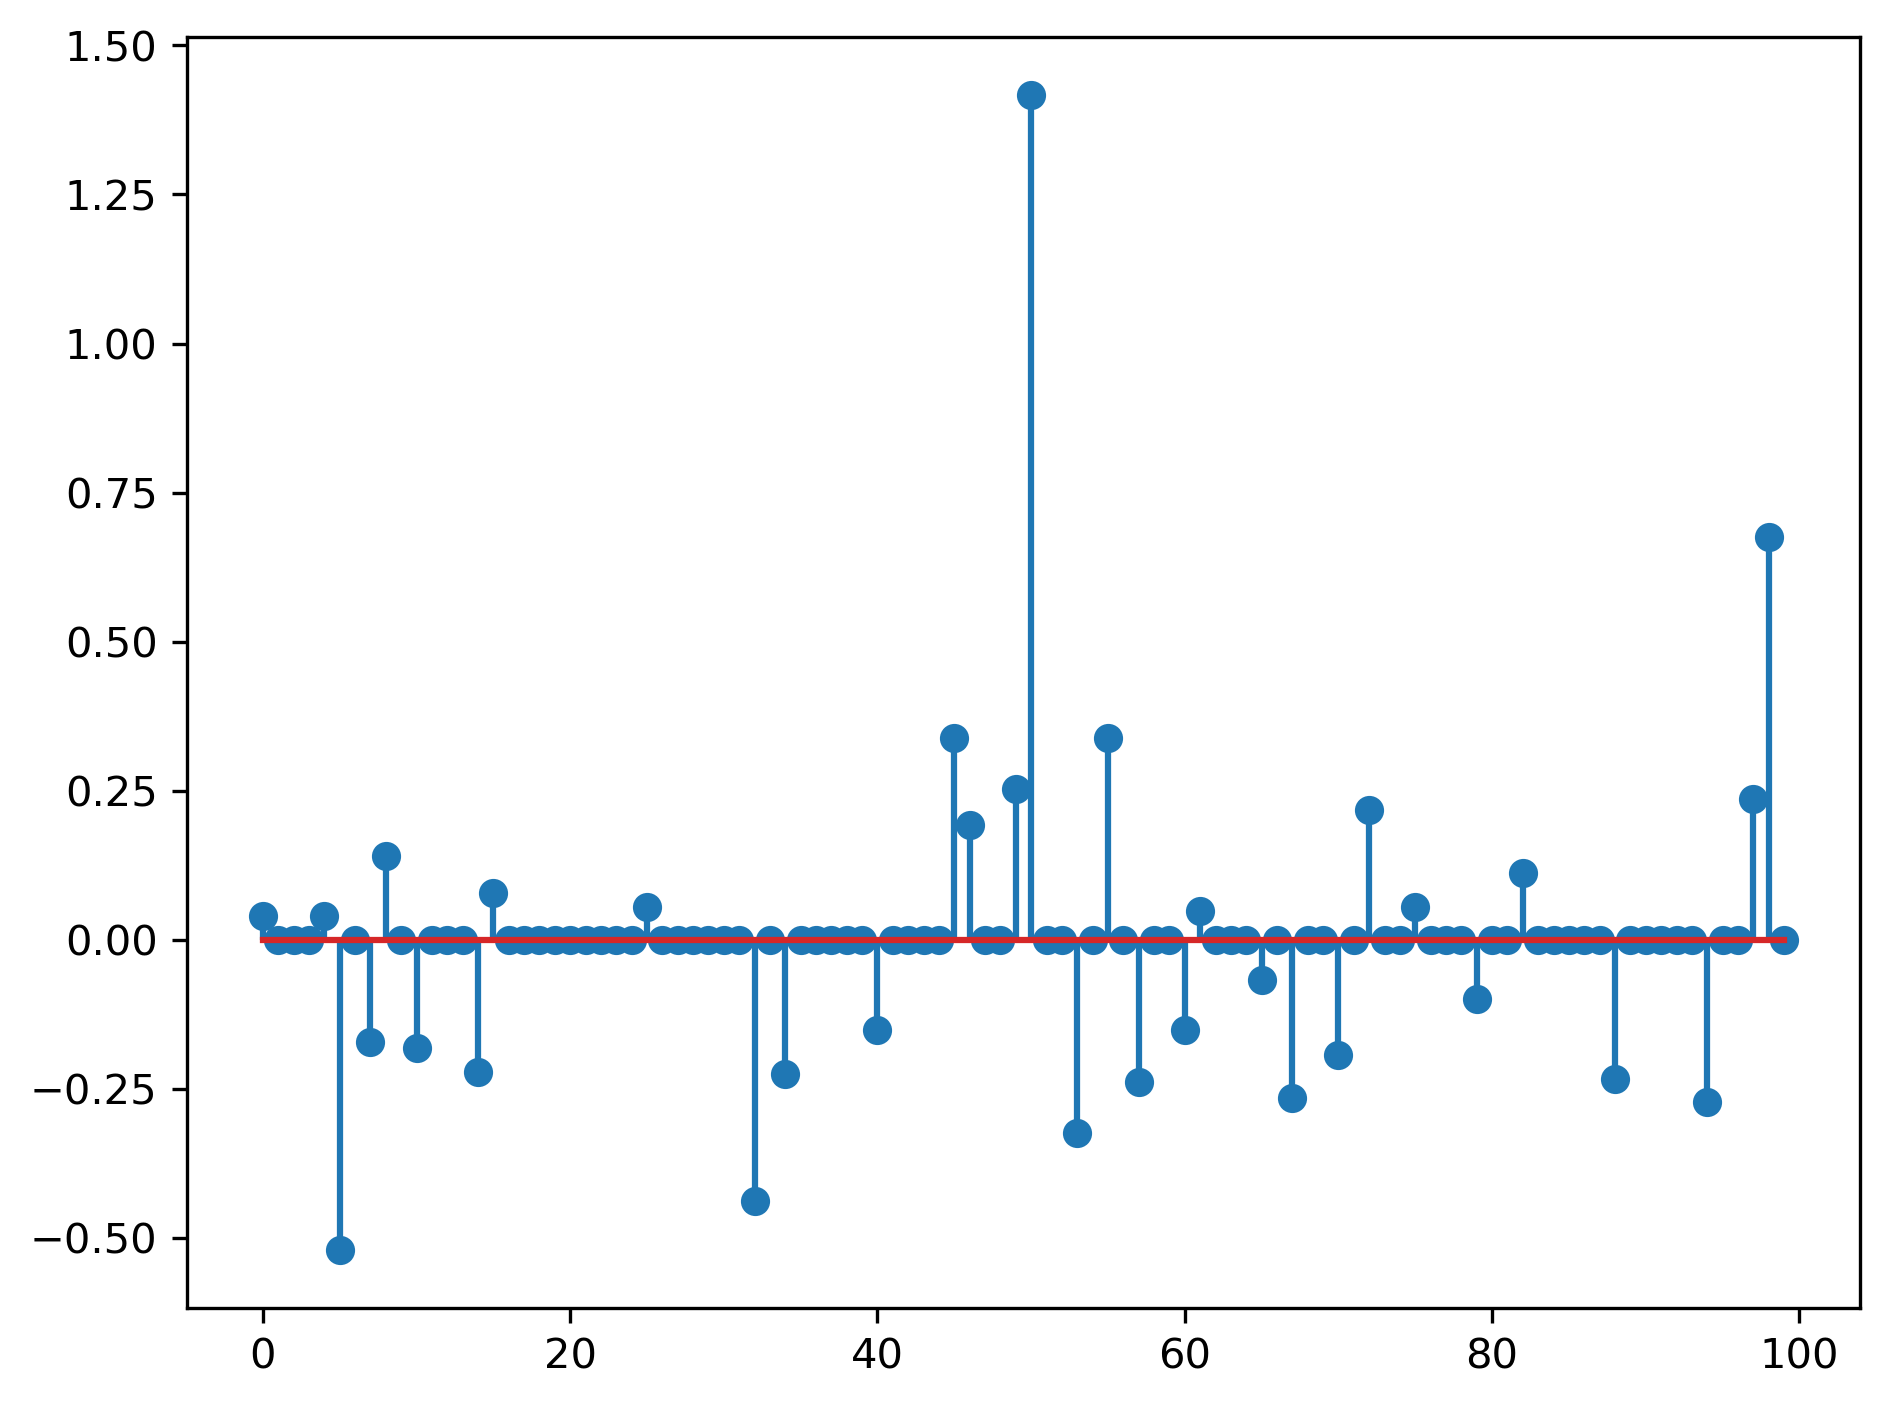
\includegraphics[width=\linewidth]{figs/q2b_randomly_subsampled_signal_fft.png}
        \caption{Random Sampling - Frequency Domain}
        \label{fig:random_subsampled_signal_fft}
    \end{subfigure}%
    \begin{subfigure}{.45\textwidth}
        \centering
        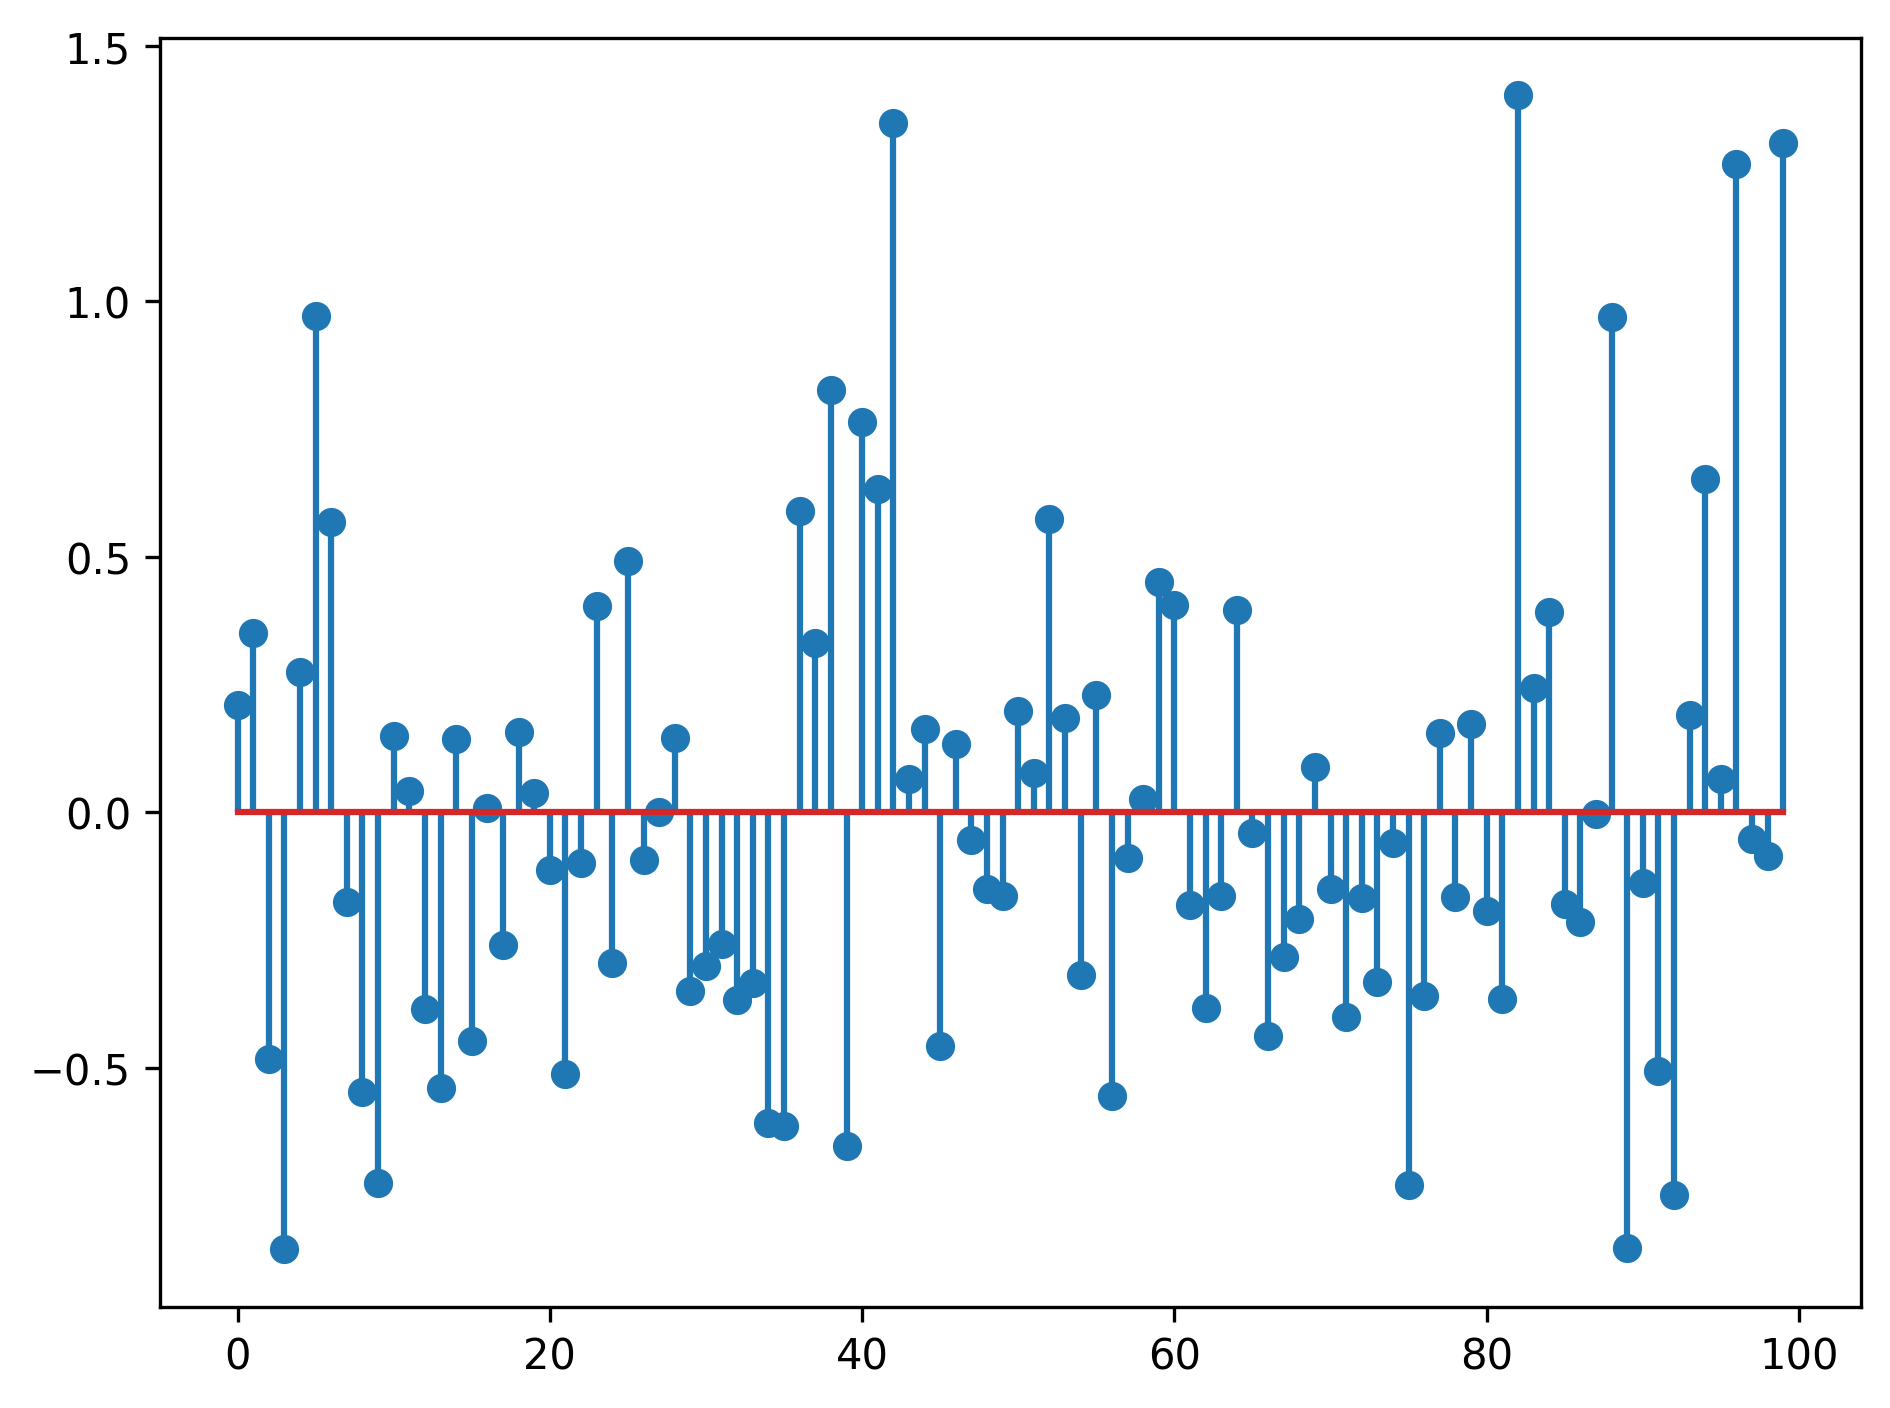
\includegraphics[width=\linewidth]{figs/q2b_randomly_subsampled_signal.png}
        \caption{Random Sampling - Time Domain}
        \label{fig:random_subsampled_signal}
    \end{subfigure}
    
    \caption{Comparison of uniformly and randomly subsampled \( y \) in both the non-sparse and sparse domains. Top row: Uniform sampling in (a) Fourier domain and (b) time domain. Bottom row: Random sampling in (c) Fourier domain and (d) time domain.}
    \label{fig:compressed_sensing_sub_sampled_signals_combined}
\end{figure}

\subsubsection{Results}
Using iterative soft thresholding and enforcing consistency in the measurement domain, the original sparse signal \( s \) is reconstructed from the sub sampled measurements \( y \). The reconstructed signals under uniform and random sampling strategies are shown in Figure \ref{fig:full_comparison}. The reconstructed signals in the frequency domain are shown in Figure \ref{fig:full_comparison}.

\begin{figure}[H]
    \centering
    % Original Signal Subfigures
    \begin{subfigure}{.45\textwidth}
        \centering
        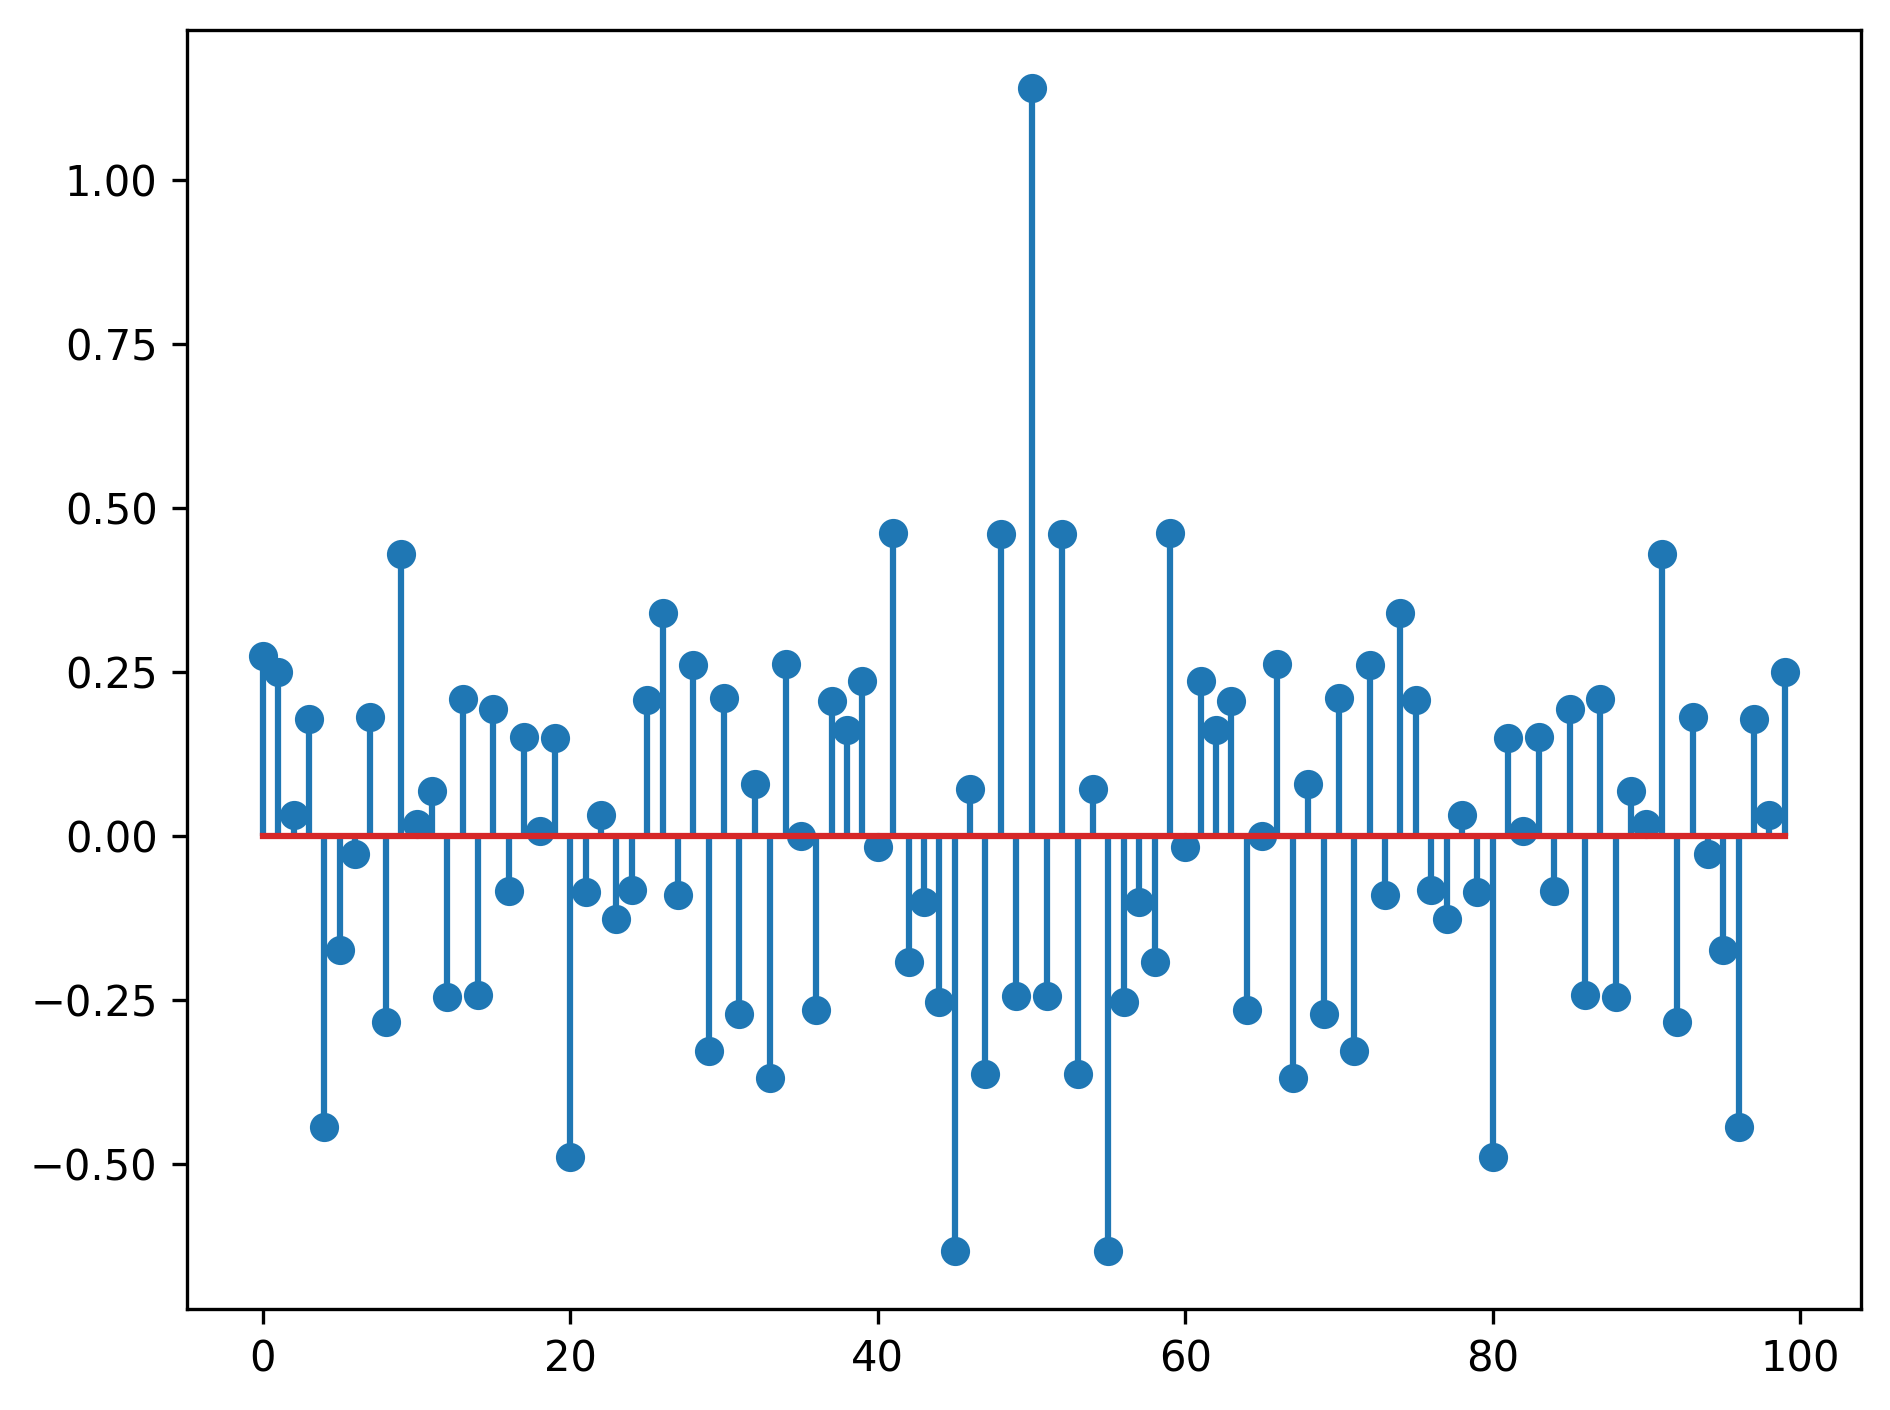
\includegraphics[width=\linewidth]{figs/q2b_original_sparse_signal_fft.png}
        \caption{Original - Frequency}
        \label{fig:original_signal_fft}
    \end{subfigure}%
    \begin{subfigure}{.45\textwidth}
        \centering
        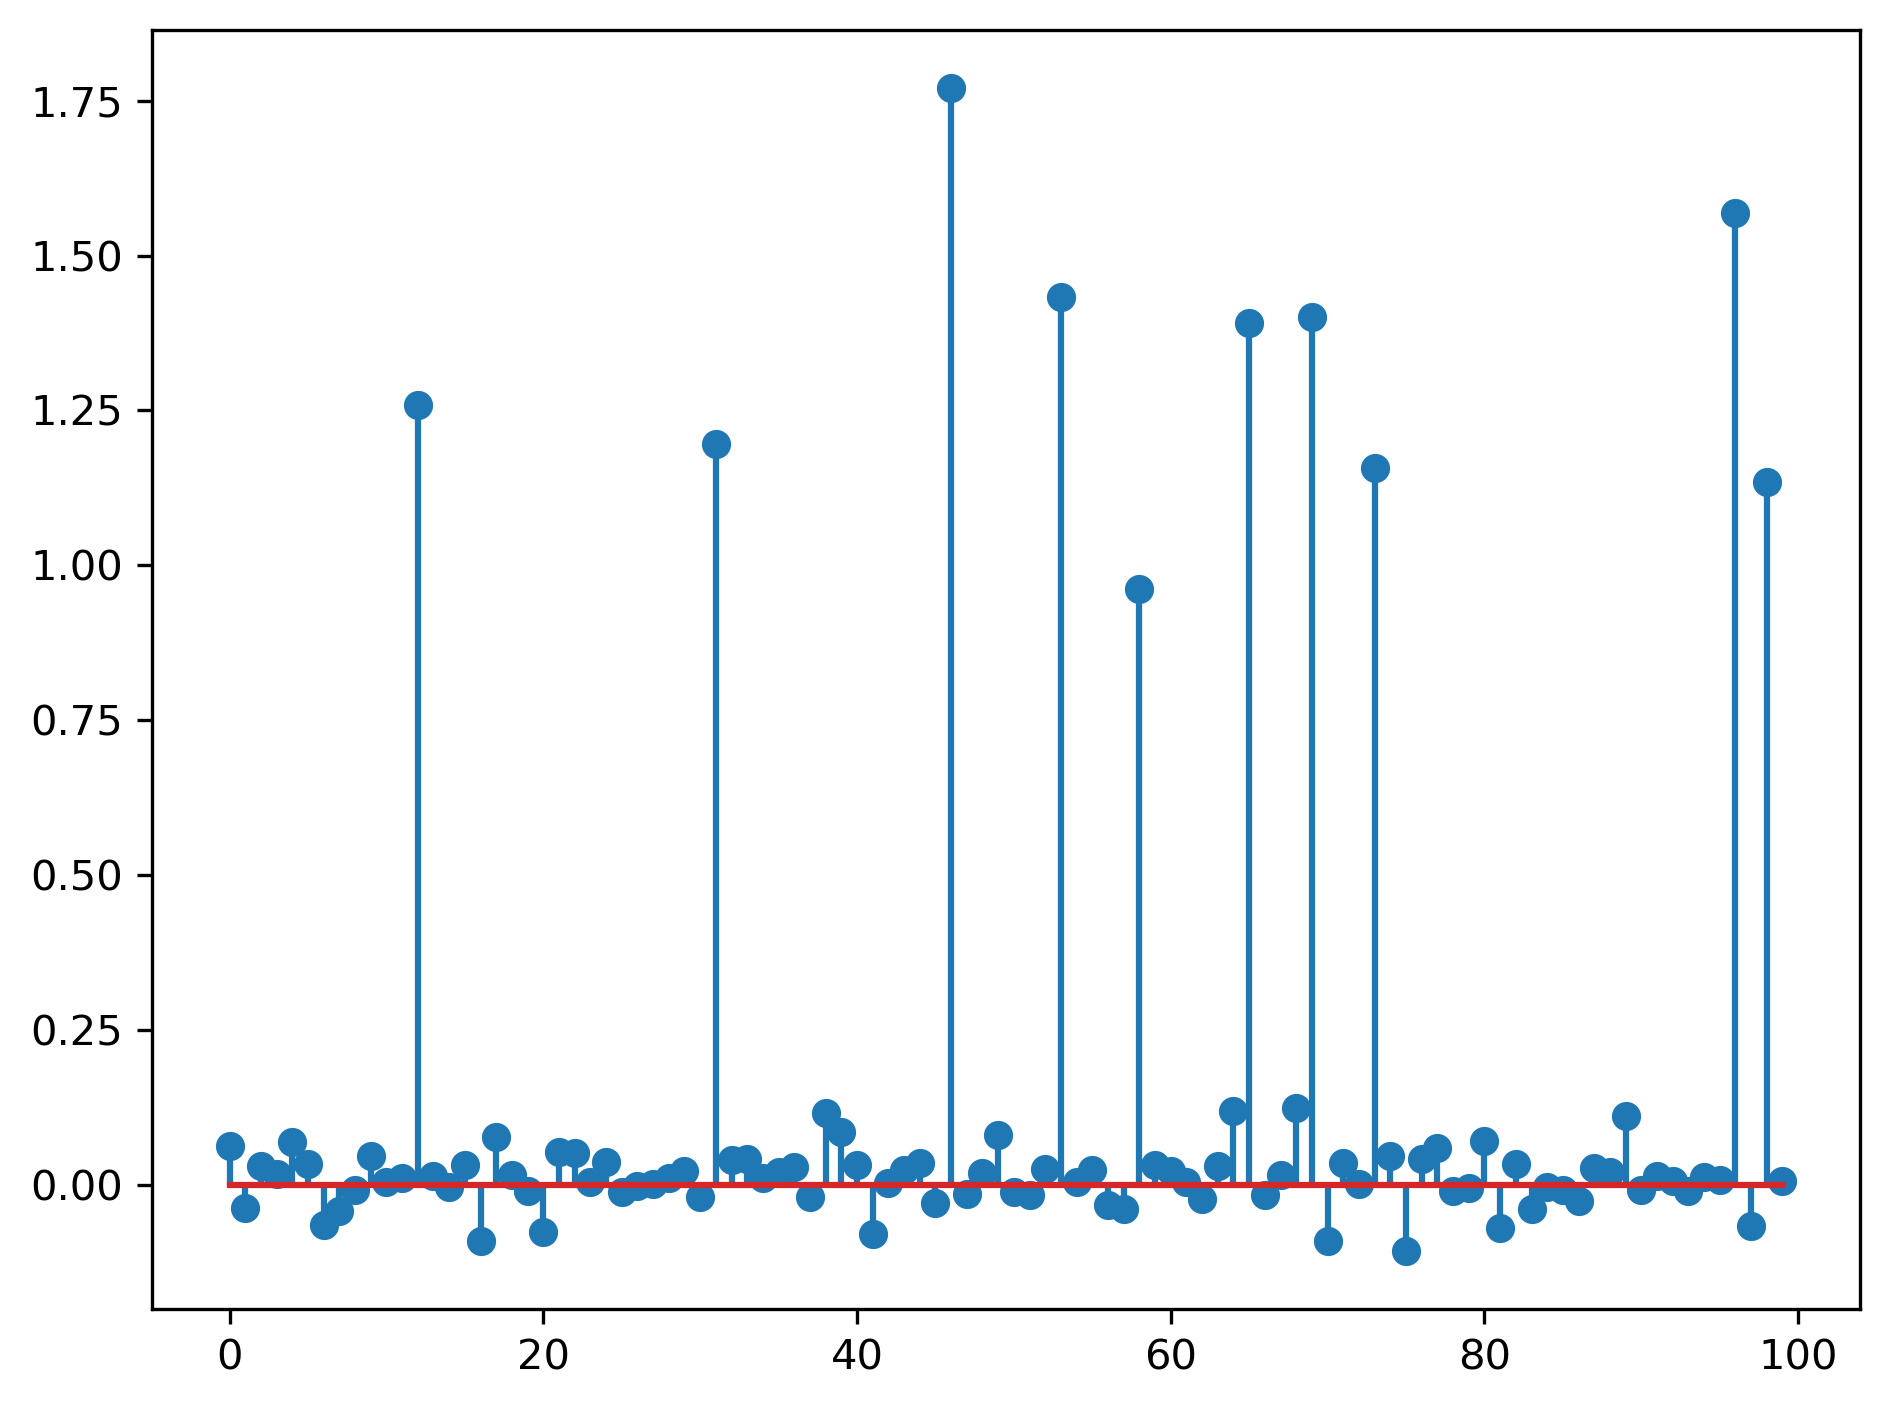
\includegraphics[width=\linewidth]{figs/q2b_original_sparse_signal.png}
        \caption{Original - Time}
        \label{fig:original_signal}
    \end{subfigure}

    % Reconstructed Signal Subfigures
    \begin{subfigure}{.45\textwidth}
        \centering
        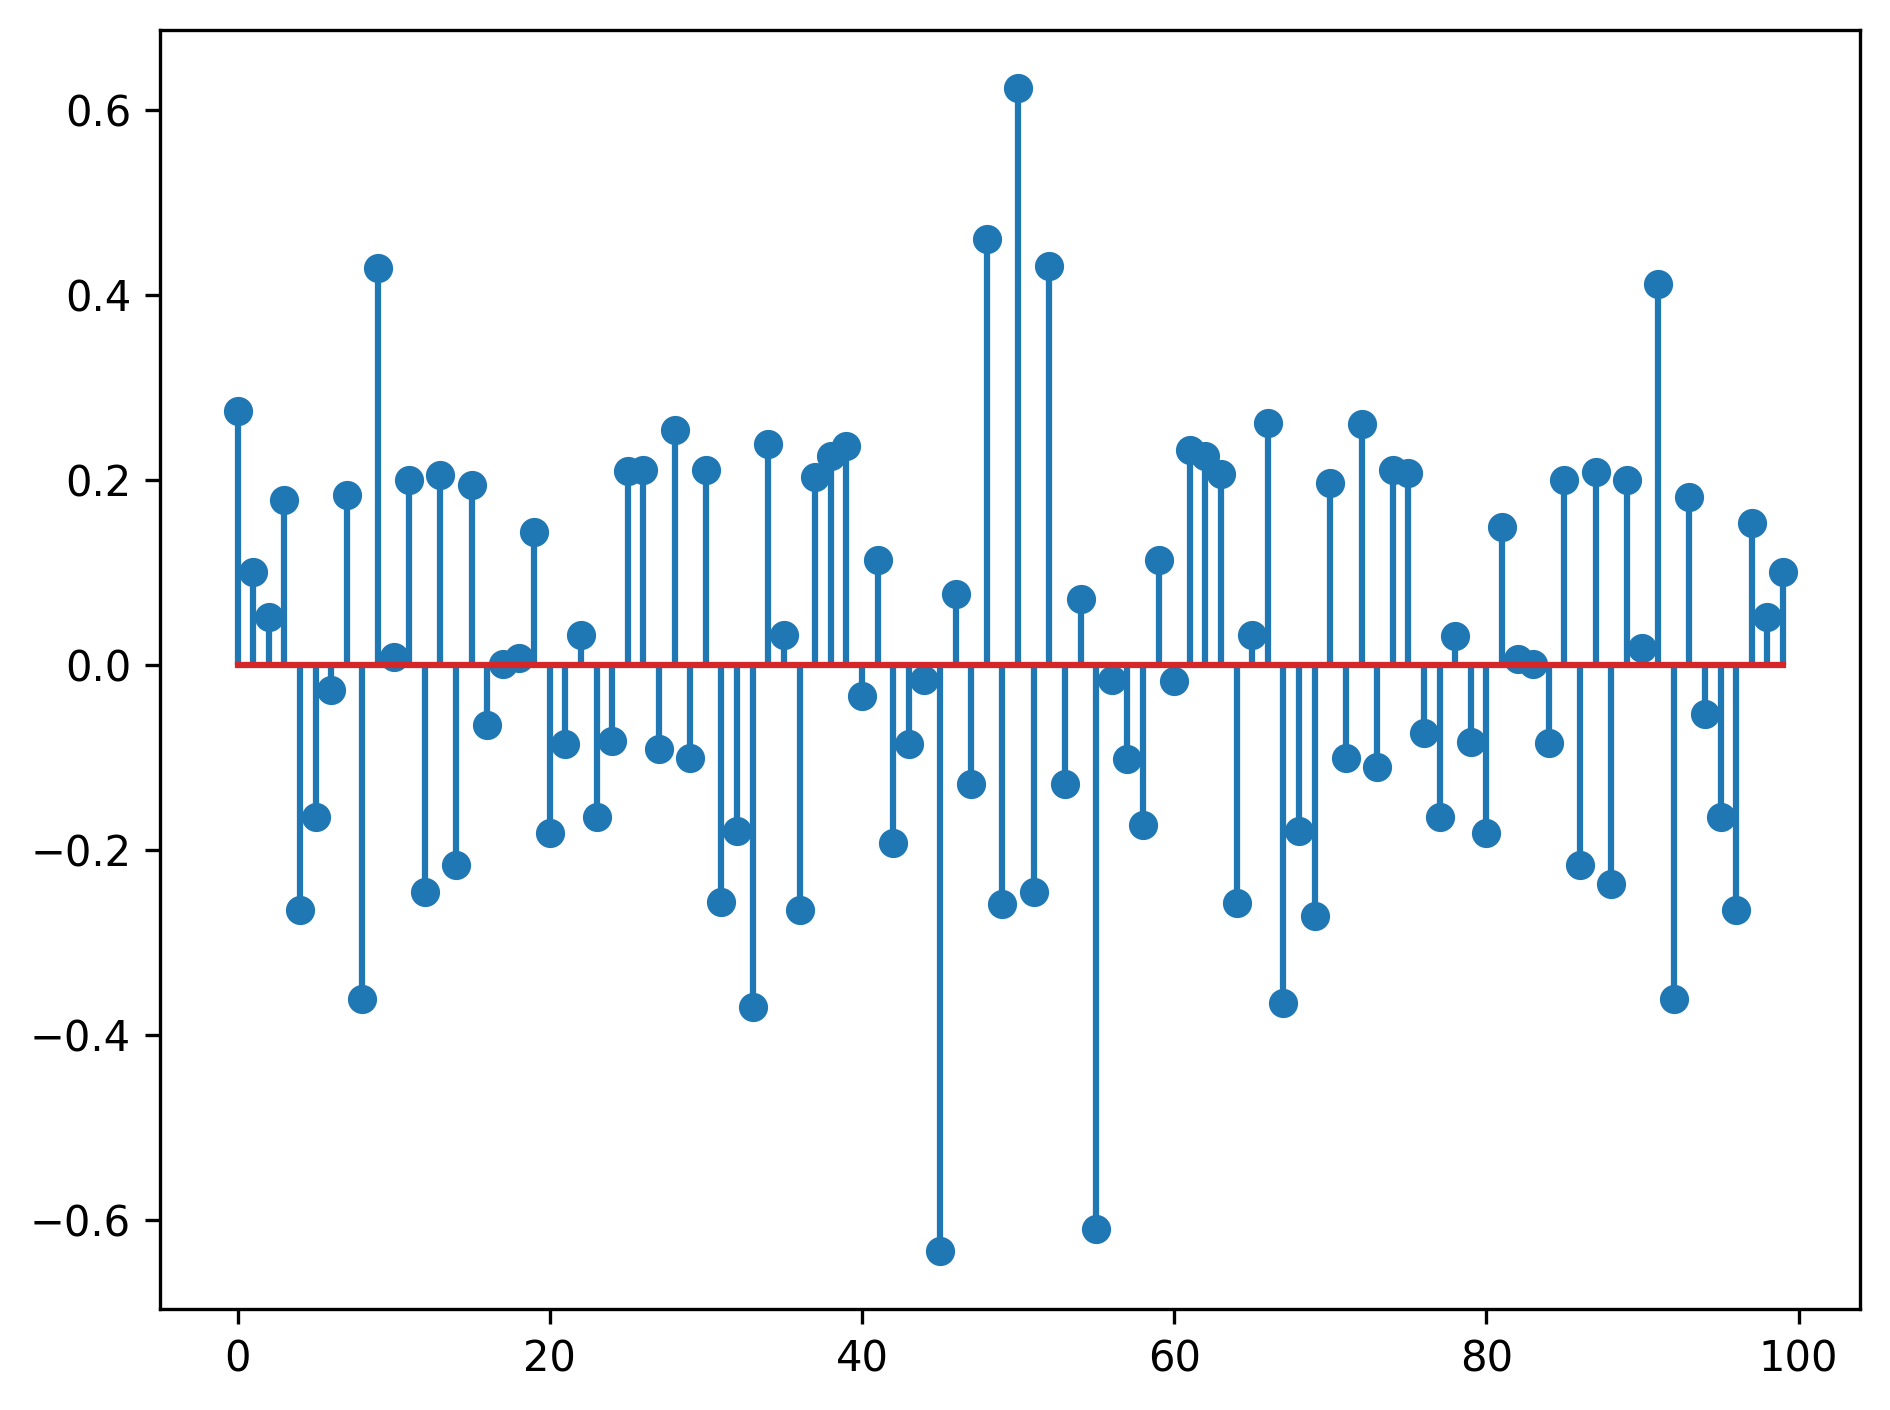
\includegraphics[width=\linewidth]{figs/q2b_uniformly_recovered_signal_fft.png}
        \caption{Reconstructed (Uniform) - Frequency}
        \label{fig:uniform_reconstructed_signal_fft}
    \end{subfigure}%
    \begin{subfigure}{.45\textwidth}
        \centering
        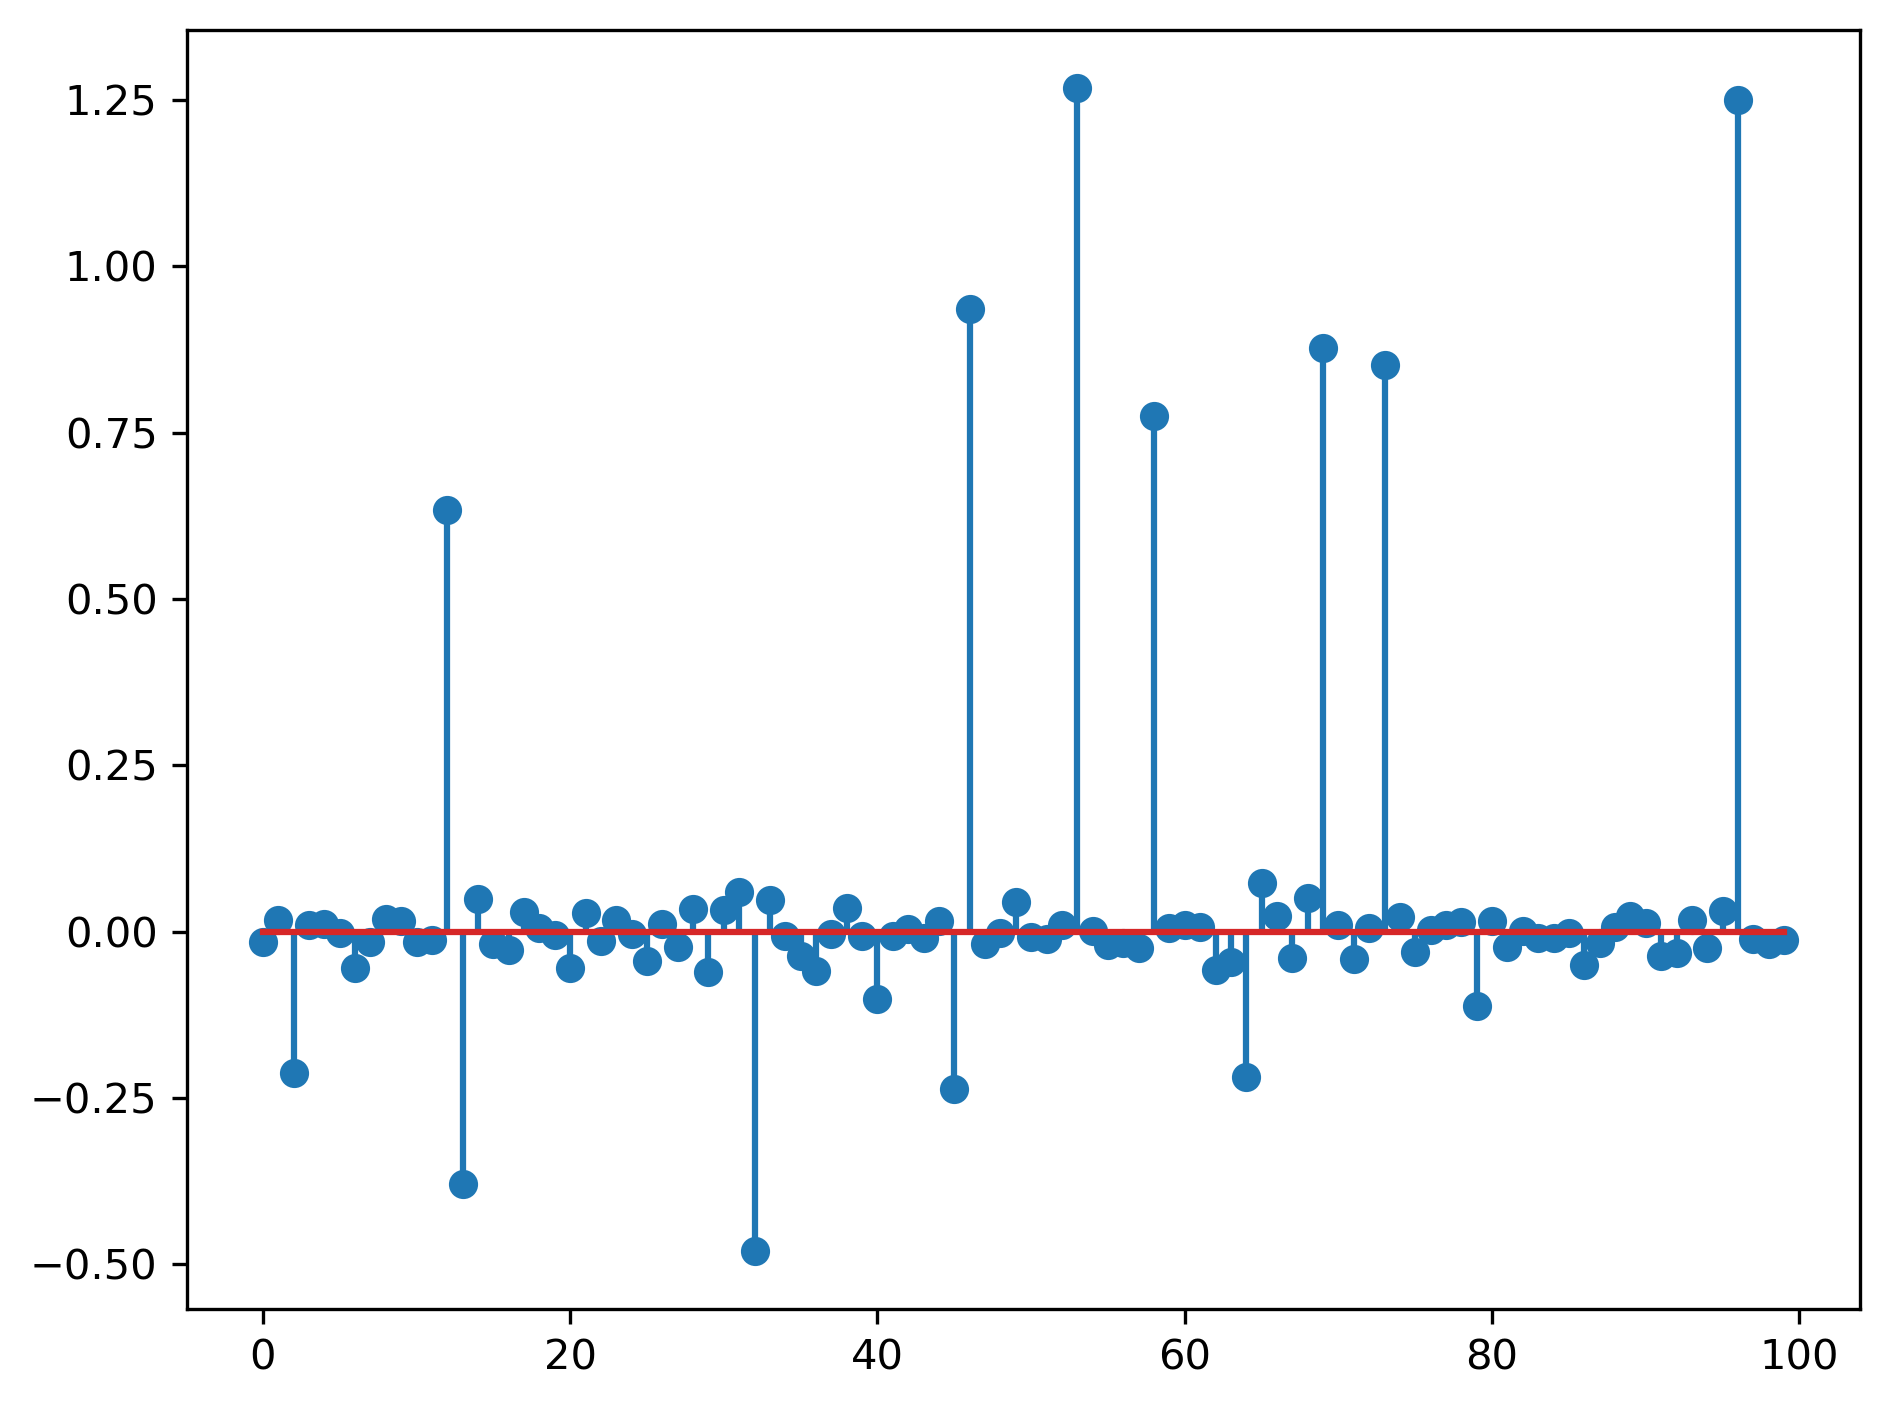
\includegraphics[width=\linewidth]{figs/q2b_uniformly_recovered_signal.png}
        \caption{Reconstructed (Uniform) - Time}
        \label{fig:uniform_reconstructed_signal}
    \end{subfigure}
    
    \begin{subfigure}{.45\textwidth}
        \centering
        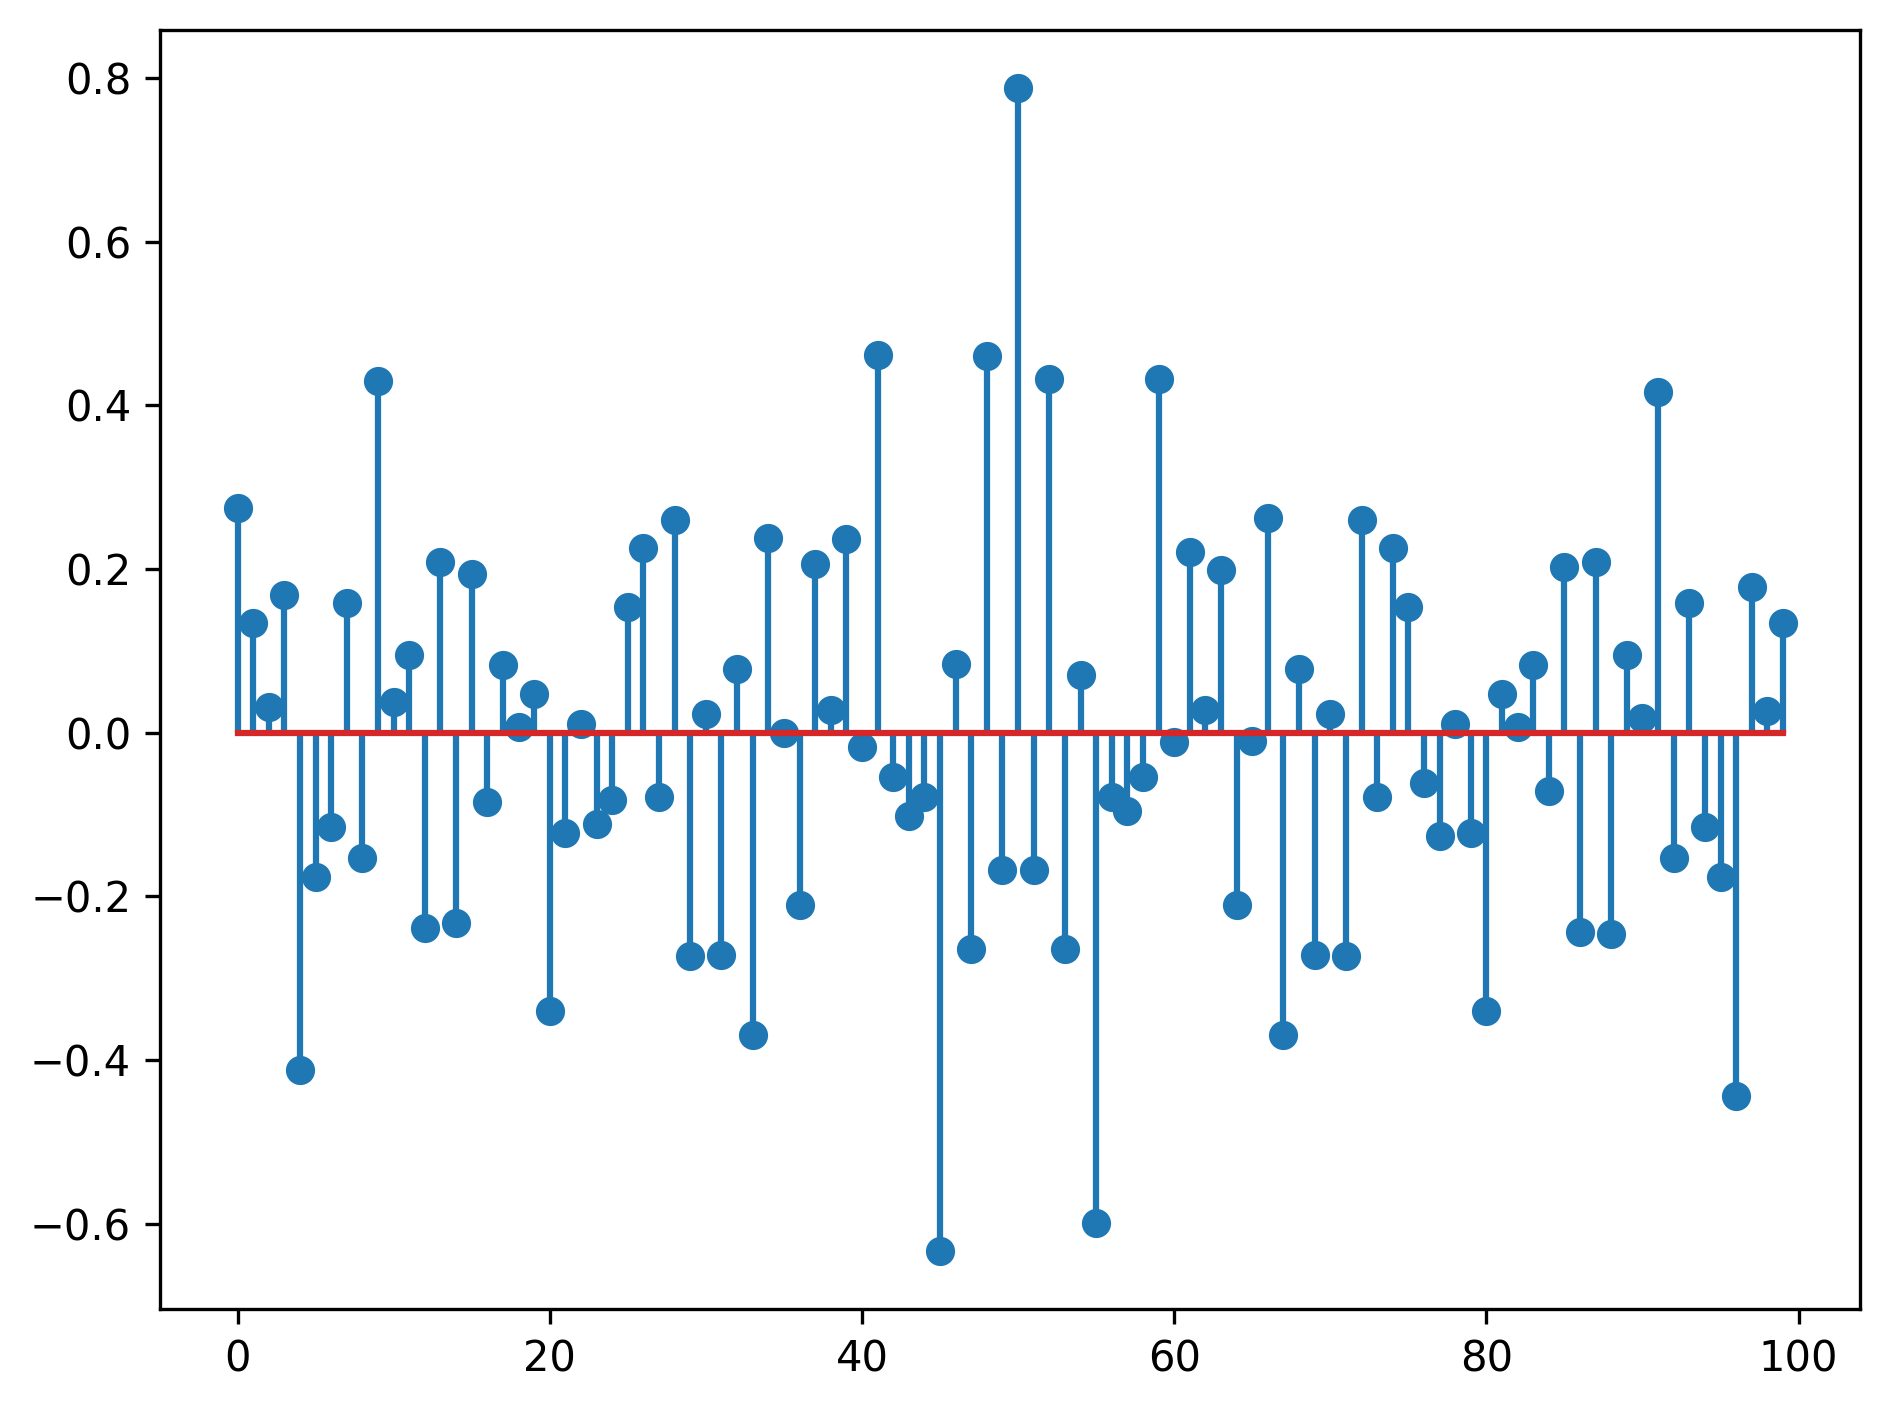
\includegraphics[width=\linewidth]{figs/q2b_randomly_recovered_signal_fft.png}
        \caption{Reconstructed (Random) - Frequency}
        \label{fig:random_reconstructed_signal_fft}
    \end{subfigure}%
    \begin{subfigure}{.45\textwidth}
        \centering
        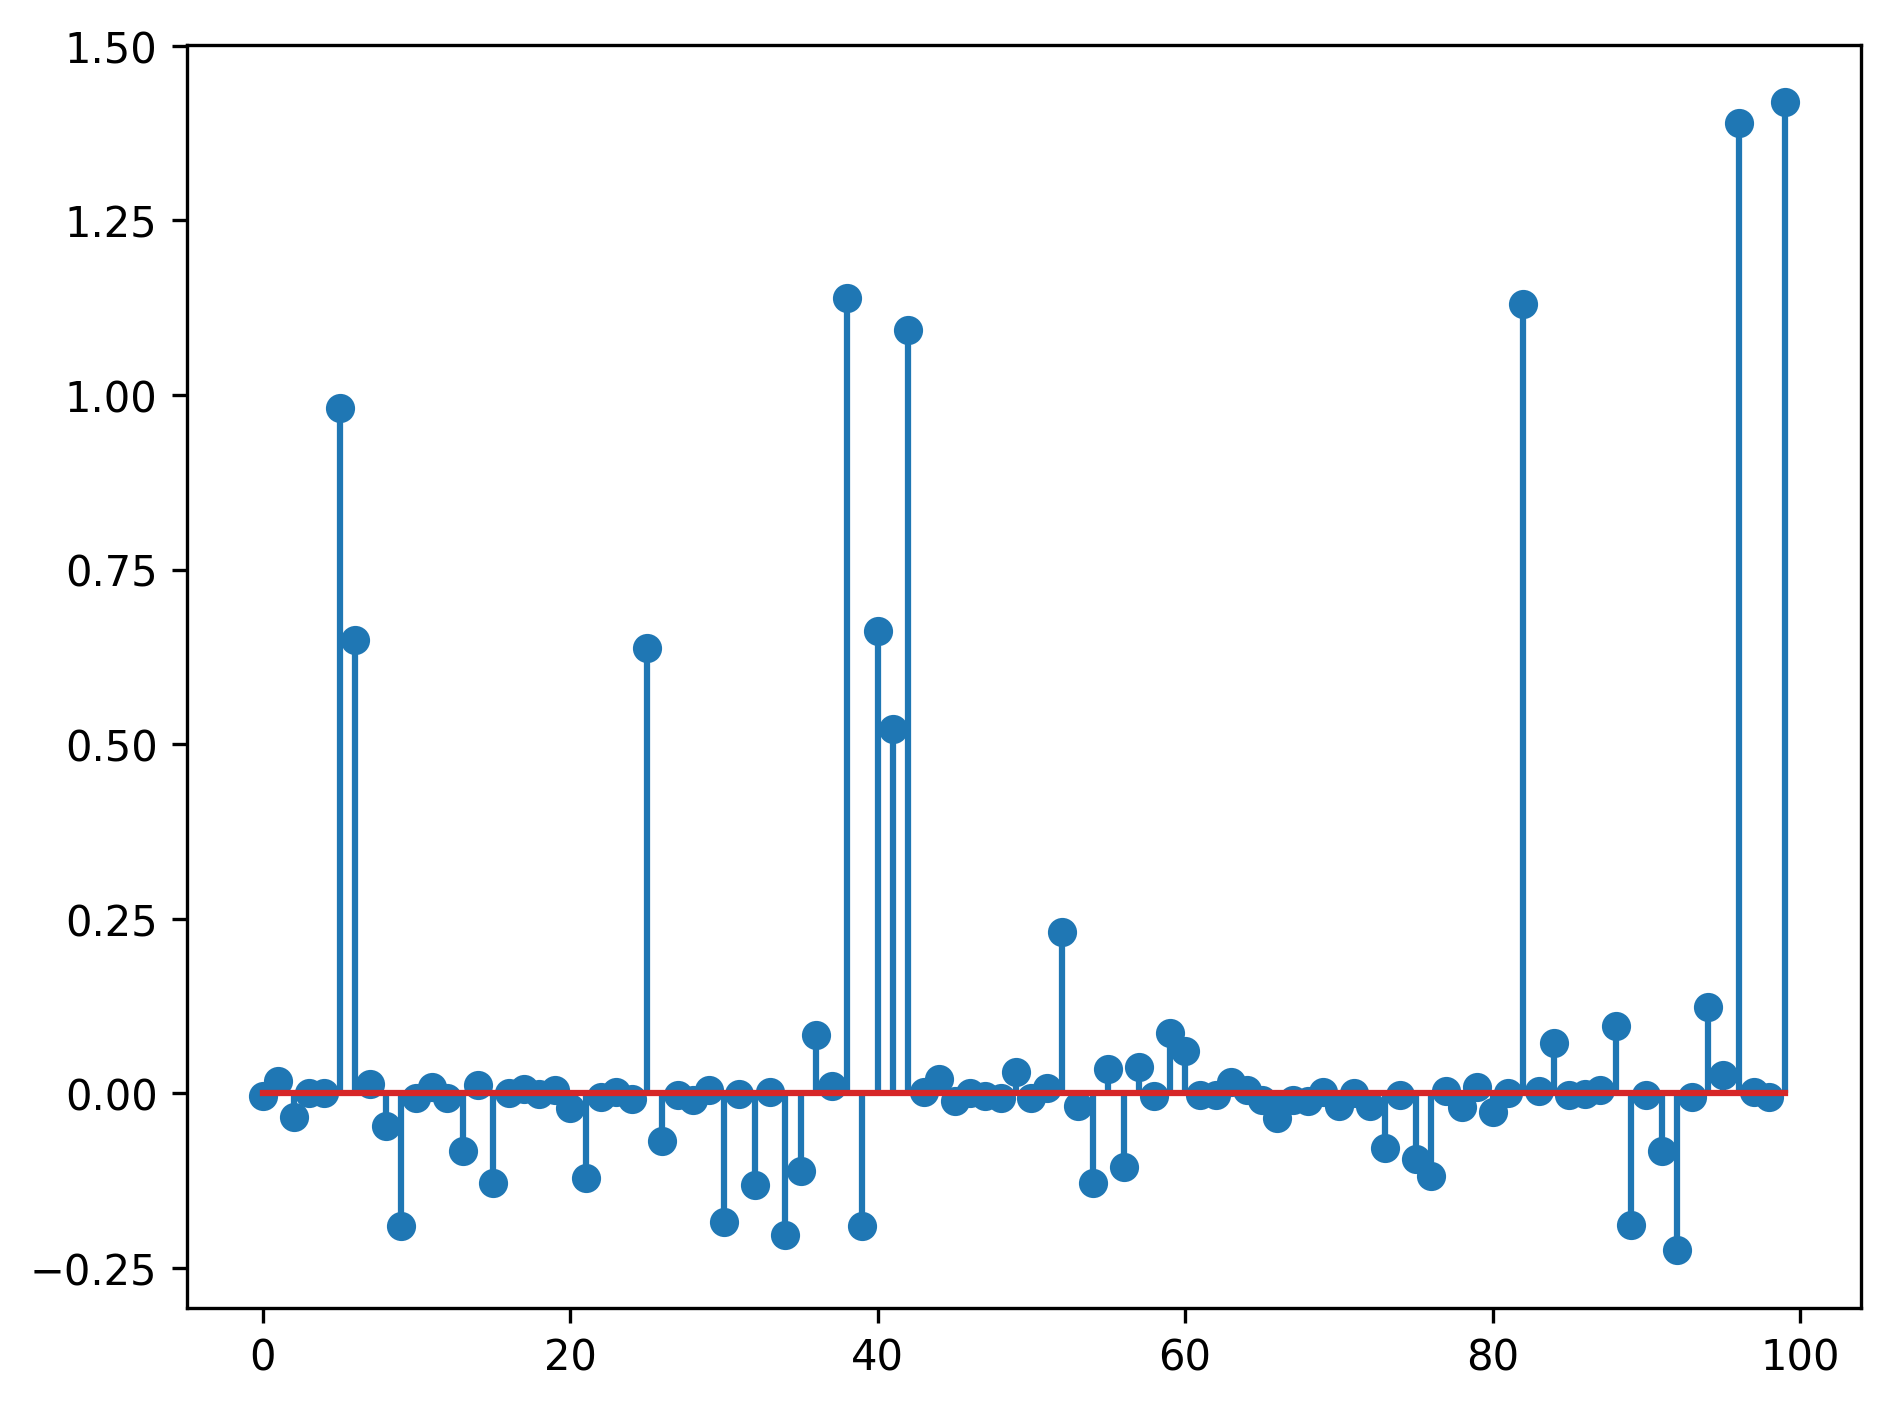
\includegraphics[width=\linewidth]{figs/q2b_randomly_recovered_signal.png}
        \caption{Reconstructed (Random) - Time }
        \label{fig:random_reconstructed_signal}
    \end{subfigure}
    
    \caption{Comparison of the original and reconstructed signals under uniform and random sampling strategies in both the non-sparse and sparse domains.}
    \label{fig:full_comparison}
\end{figure}

It is clear from the results that the reconstruction has been successful for both the uniform and random sampling strategies. With the random sampling strategy presenting a better reconstruction.
\subsubsection{Discussion}



% Explain how regularisation can be used to solve the problem and why L1 norm is used.

% Describe how there is still some conditions on the number of measurements we need for faithful reconstruction.

% Introduce the signal 

\subsection{Part C - Compressed Reconstruction and Multi-resolution Analysis}
This question focuses on the reconstruction of the image shown in Fig \ref{fig:river_side}, using a varying subset of its wavelet coefficients. The motivation is to demonstrate how natural images can have sparse representations in the another domain.
\begin{figure}[H]
    \centering
    \includegraphics[width=0.8\textwidth]{../data/river_side.jpeg}
    \caption{River side image.}
    \label{fig:river_side}
\end{figure}

\subsection{Discrete Wavelet Transform of the Image}
The image first cropped to remove the white space padding and then transformed into the wavelet domain using the discrete wavelet transform (DWT) using the Daubechies wavelet as the mother wavelet and 3 levels of frequency decomposition. To visualize the wavelet coefficients, they are thresholded to retain only the top 15\% of the coefficients. These are shown in Fig \ref{fig:wavelet_coefficients}, where the coefficients corresponding to various frequency scales are stacked in a hierarchical fashion. The upper-left quadrant represents the low-frequency components,  The remaining quadrants display higher frequency details at various orientations (horizontal, vertical, and diagonal). The most significant point is how most of the energy is concentrated in the low-frequency components, while the high-frequency components show more sparse activation, illustrating the sparsity of natural images in the wavelet domain.

\begin{figure}[H]
    \centering
    \includegraphics[width=0.55\textwidth]{figs/q2c_river_side_wavelet_transform.jpeg}
    \caption{Thresholded Daubechies wavelet transform of the river side image, showing the top 15\% coefficients for 3 levels of decomposition.}
    \label{fig:wavelet_coefficients}
\end{figure}

The image can be reconstructed using the inverse DWT. The original, reconstruction and difference images are shown in Fig \ref{fig:full_reconstruction}, the negligible mean squared error between the reconstruction and original image illustrates how near perfect reconstruction can be achieved from the discrete set of wavelet coefficients. 

\begin{figure}[H]
    \centering
    \begin{subfigure}{.45\textwidth}
        \centering
        \includegraphics[width=\linewidth]{figs/q2c_river_side_original.jpeg}
        \caption{Original Image}
        \label{fig:original_image}
    \end{subfigure}%
    \begin{subfigure}{.45\textwidth}
        \centering
        \includegraphics[width=\linewidth]{figs/q2c_river_side_reconstructed.jpeg}
        \caption{Reconstructed Image}
        \label{fig:reconstructed_image}
    \end{subfigure}%
    
    \begin{subfigure}{.45\textwidth}
        \centering
        \includegraphics[width=\linewidth]{figs/q2c_river_side_difference.jpeg}
        \caption{Difference Image}
        \label{fig:difference_image}
    \end{subfigure}%
    \caption{Comparison of the original and reconstructed river side images, along with the difference image.}
    \label{fig:full_reconstruction}
\end{figure}


\subsection{Image Reconstruction with Selective Coefficient Retention}
The reconstructed images, displayed in Figure~\ref{fig:thresholded_reconstruction}, result from retaining varying percentages of the largest wavelet coefficients---20\%, 10\%, 5\%, and 2.5\%. A discrete wavelet transform with two levels of decomposition is employed to make the effect of  the coefficient retention more pronounced. It is apparent that the quality of reconstruction diminishes as fewer coefficients are retained, particularly affecting areas of the image rich in high-frequency details. Remarkably, even with only 10\% of the coefficients preserved, the image reconstruction remains a highly accurate depiction of the original, underscoring the inherent sparsity of natural images in the wavelet domain.

\begin{figure}[H]
    \centering
    \begin{subfigure}{.9\textwidth}
        \centering
        \includegraphics[width=\linewidth]{figs/q2c_river_side_threshold_0_2.jpeg}
        \caption{Reconstruction with top 20\% of coefficients retained}
        \label{fig:reconstructed_20}
    \end{subfigure}
    
    \begin{subfigure}{.9\textwidth}
        \centering
        \includegraphics[width=\linewidth]{figs/q2c_river_side_threshold_0_1.jpeg}
        \caption{Reconstruction with top 10\% of coefficients retained}
        \label{fig:reconstructed_10}
    \end{subfigure}
    
    \begin{subfigure}{.9\textwidth}
        \centering
        \includegraphics[width=\linewidth]{figs/q2c_river_side_threshold_0_05.jpeg}
        \caption{Reconstruction with top 5\% of coefficients retained}
        \label{fig:reconstructed_5}
    \end{subfigure}
    
    \begin{subfigure}{.9\textwidth}
        \centering
        \includegraphics[width=\linewidth]{figs/q2c_river_side_threshold_0_025.jpeg}
        \caption{Reconstruction with top 2.5\% of coefficients retained}
        \label{fig:reconstructed_2_5}
    \end{subfigure}
    
    \caption{Reconstruction of the river side image using varying levels of coefficient retention.}
    \label{fig:thresholded_reconstruction}
\end{figure}

\section{Question 3 - Solving inverse problems}
\subsection{Part A - Convergence Rate of Gradient Descent}
% Introduce problem objective - function, set up, goal
In this exercise, the function $ f : \mathbb{R}^2 \rightarrow \mathbb{R} $ is considered, defined as $ f(\mathbf{x}) = \frac{1}{2} x_1^2 + x_2^2 $. The task is to minimise the function using gradient descent, starting from the initial point $ \mathbf{x}_0 = \begin{bmatrix} 1 \\ 1 \end{bmatrix} $. The goal is to theoretically determine the number of iterations $ K $ required to achieve a specified accuracy, defined as $ f(x) - f(x_*)$ where $x_*$ is the optimal solution, less than $ 0.01 $. This prediction is then compared to computational results.

\subsubsection{Proving \(f \) is Convex}
First the function convexity is verified by considering the Hessian matrix of \( f \): 
\[
H_f(\mathbf{x}) = \begin{bmatrix} 1 & 0 \\ 0 & 2 \end{bmatrix}
\]
This matrix is constant and has positive eigenvalues (1 and 2) for all \( \mathbf{x} \in  \mathbb{R}^2 \), indicating that \( f \) is convex over the entire domain.

\subsubsection{Identifying the Lipschitz Constant of the Gradient of \( f \)}

The Lipschitz constant of the gradient of \( f \) is determined by considering the function \( f \) with the following gradient:
\[
\nabla f(\mathbf{x}) = \begin{bmatrix} x_1 \\ 2x_2 \end{bmatrix}.
\]

The Lipschitz constant \( L \) is derived through the application of the definition of the Lipschitz continuity property of the gradient of \( f \):
\[
\| \nabla f(\mathbf{x}) - \nabla f(\mathbf{x'}) \|_2 \leq L \| \mathbf{x} - \mathbf{x'} \|_2,
\]
where \( \mathbf{x} \) and \( \mathbf{x'} \) represent any two points in the domain of \( f \). 

The norm of the gradient difference is calculated as follows:
\[
\| \nabla f(\mathbf{x}) - \nabla f(\mathbf{x'}) \|_2 = \left\| \begin{bmatrix} x_1 - x'_1 \\ 2x_2 - 2x'_2 \end{bmatrix} \right\|_2 = \sqrt{(x_1 - x'_1)^2 + 4(x_2 - x'_2)^2}.
\]

\[
\sqrt{(x_1 - x'_1)^2 + 4(x_2 - x'_2)^2} \leq \sqrt{4} \cdot \sqrt{(x_1 - x'_1)^2 + (x_2 - x'_2)^2} = 2 \cdot \|\mathbf{x} - \mathbf{x'}\|_2.
\]

To confirm rigorously that any constant \( L < 2 \) does not satisfy the Lipschitz continuity property, specific vectors \( \mathbf{x} \) and \( \mathbf{x'} \) are considered such that the inequality is challenged. Specifically, if \( \mathbf{x} = \begin{bmatrix} 0 \\ x_2 \end{bmatrix} \) and \( \mathbf{x'} = \begin{bmatrix} 0 \\ x'_2 \end{bmatrix} \) are selected, where \( x_2 \) and \( x'_2 \) are any real numbers, the following is observed:
\[
\| \nabla f(\mathbf{x}) - \nabla f(\mathbf{x'}) \|_2 = 2 |x_2 - x'_2| = 2 \|\mathbf{x} - \mathbf{x'}\|_2.
\]

\[
2 \|\mathbf{x} - \mathbf{x'}\|_2 > L \|\mathbf{x} - \mathbf{x'}\|_2 \quad \forall L < 2.
\]
Therefore, it is shown that for \( L < 2 \), the inequality does not hold.

\subsubsection{Finding the Optimal Solution}
The next step is to identify the optimal solution \( \mathbf{x}^* \) of the function \( f \) by solving the gradient equation. \( \nabla f(\mathbf{x}) = \mathbf{0} \). The gradient of \( f \) is given by:
\[
\nabla f(\mathbf{x}) = \begin{bmatrix} x_1 \\ 2x_2 \end{bmatrix}.
\]
The single solution to this system of equations are \( x_1 = 0 \) and \( x_2 = 0 \), thus there is a single optimal solution at the origin \( \mathbf{x}^* = \begin{bmatrix} 0 \\ 0 \end{bmatrix} \).

\subsection{Theoretical Convergence Rate}
Now that \(f\) is confirmed to be convex and the Lipschitz constant of the gradient is determined, the following bound for a convex and L-smooth can be used:
$$
    f(\mathbf{x}_K) - f(\mathbf{x}_*) \leq \frac{L \|\mathbf{x}_0 - \mathbf{x}^*\|_2^2}{2K},
$$

Thus, the above inequality can be rearranged to give a bound on the number of iterations $K$ to achieve the desired accuracy. 
\[
K \leq \frac{L \|\mathbf{x}_0 - \mathbf{x}^*\|_2^2}{2(f(\mathbf{x}_K) - f(\mathbf{x}^*))}
\]

Substituting the values of \( L = 2 \), \( \|\mathbf{x}_0 - \mathbf{x}^*\|^2_2 = 2 \) and \(f(\mathbf{x}_K) - f(\mathbf{x}^*) = 0.01 \) into the equation, the theoretical number of iterations required to achieve the specified accuracy is calculated as \( K \leq 200 \).

\subsection{Practical Convergence Rate}
To practically determine the number of iterations required to achieve the specified accuracy, the gradient descent algorithm is implemented in Python with a learning rate of \( \alpha = \frac{1}{L} = \frac{1}{2} \). The algorithm is run starting at 
\( \mathbf{x}_0 = \begin{bmatrix} 1 \\ 1 \end{bmatrix} \) and iterated until the difference between the function at the current point and the optimal solution is less than 0.01. The number of iterations required to achieve this accuracy is found to be 3, which while consistent with the theoretical prediction, is two orders of magnitude lower.

\subsection{Strong Convexity of the Function}
The primary reason for the observed convergence rate being significantly lower than the theoretical bound is that the strong convexity of the function has not considered. A function \( f \) is strongly convex with parameter \( \mu \) if the following holds:
\[
\nabla^2 f(\mathbf{x}) \succeq \mu \mathbf{I} \quad \forall \mathbf{x} \in \mathbb{R}^2,
\]
where \( \nabla^2 f(\mathbf{x}) \) is the Hessian matrix of \( f \) and \( \mathbf{I} \) is the identity matrix. The Hessian matrix of \( f \) is given by:
\[
H_f(\mathbf{x}) = \begin{bmatrix} 1 & 0 \\ 0 & 2 \end{bmatrix}.
\]

Which is equivalent to stating that \( H_f(\mathbf{x}) - \mu \mathbf{I} \) must be positive semi-definite for all \( \mathbf{x} \in \mathbb{R}^2 \). The smallest value of \( \mu \) that satisfies this condition is 1.

Now that \( f \) is confirmed to be strongly convex with \( \mu = 1 \), the following bound for a strongly convex and L-smooth function can be used:
% Derive the convergence rate if word count available.

\[
\|\mathbf{x}_K - \mathbf{x}^*\|_2^2 \leq \left(1 - \frac{\mu}{L}\right)^K \|\mathbf{x}_0 - \mathbf{x}^*\|_2^2
\]

This can be seen to give a convergence rate of $\mathcal{O}\left(\frac{1}{\epsilon}\right)$, where $\epsilon$ is the desired accuracy. In this case the convergence rate order evaluates to approximately 5 which is more consistent with the practical results.

\subsection{Part B - Data Driven and Model Driven Reconstruction}
This exercise compares the performance of data-driven and model-driven approaches for solving the image reconstruction inverse problem. Here the goal is to minimise the objective function:
\[
\min_{\mathbf{x}} \left\| \mathbf{y} - \mathbf{A} \mathbf{x} \right\|_2^2 + \lambda \left\| \mathbf \nabla \mathbf{x} \right\|_1,
\]
where in this context \( \mathbf{A} \) is the CT forward operator, \( \mathbf{y} \) is the observed noisy sinogram, \( \mathbf{x} \) is the true image to be reconstructed, and \( \lambda \) is the regularisation parameter. The particular choice of regularisation is known as the total variation (TV) regularisation, which promotes sparsity in the gradient of the image. 
\subsubsection{Model-Driven Approach}
Such a problem would typically be solved using proximal gradient descent however the proximal operator for the total variation regularisation is not straight forward to calculate. However, the proximal operator can be computed under a variable splitting scheme, so the problem is tackled using the alternating direction method of multipliers (ADMM) algorithm. Here a new quantity \( \mathbf{z} = \nabla \mathbf{x}\) is introduced and a penalty is added to the objective function to enforce the constraint \( \mathbf{z} = \nabla \mathbf{x} \). The ADMM algorithm is then used to solve the problem iteratively and can be summarised as follows:

\begin{algorithm}[H]
\caption{Alternating Direction Method of Multipliers (ADMM)}
\begin{algorithmic}[1]
\State \textbf{initialise:} $\mathbf{x}_0, \mathbf{z}_0, \mathbf{u}_0, \rho$
\State \textbf{define:} $L_\rho(\mathbf{x}, \mathbf{z}, \mathbf{u}) = \left\| \mathbf{y} - \mathbf{A} \mathbf{x} \right\|_2^2 + \lambda \left\| \mathbf{z} \right\|_1 + \mathbf{u}^T (\nabla \mathbf{x}-\mathbf{z})+\frac{\rho}{2} \left\| \nabla \mathbf{x} - \mathbf{z}\right\|_2^2$  \Comment{Define the augmented Lagrangian}
\While{not converged}
    % Define lp
    \State $\mathbf{x}_{k+1} \gets \min_x L_\rho(\mathbf{x}, \mathbf{z}_k, \mathbf{u}_k)$ \Comment{Update $x$ by minimizing the augmented Lagrangian}
    \State $\mathbf{z}_{k+1} \gets \min_z L_\rho(\mathbf{x}_{k+1}, \mathbf{z}, \mathbf{u}_k)$ \Comment{Update $z$ via proximal operator of $\|\cdot\|_1$}
    \State $\mathbf{u}_{k+1} \gets \mathbf{u}_k + \rho (\nabla \mathbf{x}_{k+1} - \mathbf{z}_{k+1})$ \Comment{Update the dual variable}
    \State $k \gets k + 1$
\EndWhile
\State \textbf{return} $\mathbf{x}_k, \mathbf{z}_k, \mathbf{u}_k$
\end{algorithmic}
\end{algorithm}

\subsubsection{Data-Driven Approach}
The solution for \( \mathbf{x} \) obtained using the ADMM algorithm is compared to the solution obtained using the data-driven approach of learned gradient descent. The learned gradient descent approach involves replacing the proximal operator at each iteration with a neural network that takes as input the arguments of the proximal operator and returns the output. The algorithm can be summarised as follows:


\begin{algorithm}[H]
    \caption{Learned Gradient Descent}
    \begin{algorithmic}[1]
    \State \textbf{initialize:} $\mathbf{x}_0$, $N$
    \State \textbf{define:} $f(\mathbf{x}) = \left\| \mathbf{y} - \mathbf{A} \mathbf{x} \right\|_2^2$ \Comment{Define the data fidelity term}
    \For{$k = 1$ to $N$}
        \State $\mathbf{g}_k \gets \mathbf{A}^T(\mathbf{A}\mathbf{x}_k - \mathbf{y})$ \Comment{Gradient computation}
        \State $\mathbf{dx} \gets h_k(\mathbf{x}_k, \mathbf{g}_k; \theta_k)$ \Comment{Apply learned proximal mapping}
        \State $\mathbf{x}_{k+1} \gets \mathbf{x}_k + \tau_k \mathbf{dx}$ \Comment{Update the solution}
    \EndFor
    \State \textbf{return} $\mathbf{x}_N$
    \end{algorithmic}
    \end{algorithm}

The initial estimate \( \mathbf{x}_0 \) is set to be the filtered back projection (FBP) reconstruction of the sinogram \( \mathbf{y} \). This provides a reasonable initial estimate for the image reconstruction problem.

\subsubsection{Model Architecture}
The architecture of the unrolling neural network \( h_* \) is a convolutional neural network that processes concatenated tensors of the current iterate $x$ and the gradient $u$. It comprises three convolutional layers, each with a kernel size of $3 \times 3$ and a stride of $1$. The first layer transforms 2 input channels to 32 output channels, followed by a Parametric Rectified Linear Unit (PReLU) activation. The second layer continues with 32 channels, also followed by PReLU. The final layer reduces the channel count from 32 to 1. The output of the network is delta $dx$, used to update the current estimate $x_i$ at each iteration of the learned gradient descent algorithm.

\subsection{Training}
The neural network is trained in a supervised manner using the Adam optimiser with a learning rate of $10^{-4}$, across 2000 epochs. The learned gradient descent algorithm is executed for 5 iterations, employing mean square error as the loss function, calculated between the final estimate $x_5$ and the true image $x^*$.

\subsection{Results}
The results of the model-driven and data-driven approaches are compared in Figure \ref{fig:reconstruction_comparison}. The data-driven approach is observed to produce a reconstruction with a higher level of detail, confirmed by the higher peak signal-to-noise ratio (PSNR), and structural similarity index (SSIM) compared to the model-driven approach and simple FBP reconstruction. 

\begin{figure}[H]
    \centering
    \includegraphics[width=0.8\textwidth]{figs/q3_2_results.png}
    \caption{Comparison of the FBP, model-driven, and data-driven reconstructions of the image.}
    \label{fig:reconstruction_comparison}
\end{figure}

\bibliographystyle{plain}  % Choose the style that suits your needs
\bibliography{references}  % The filename of the .bib file, without the extension
\end{document}